% $Id: msk-007.tex 9312 2021-08-07 15:46:07Z mskala $

%
% MSK 007 user/build manual
% Copyright (C) 2017  Matthew Skala
%
% This program is free software: you can redistribute it and/or modify
% it under the terms of the GNU General Public License as published by
% the Free Software Foundation, version 3.
%
% This program is distributed in the hope that it will be useful,
% but WITHOUT ANY WARRANTY; without even the implied warranty of
% MERCHANTABILITY or FITNESS FOR A PARTICULAR PURPOSE.  See the
% GNU General Public License for more details.
%
% You should have received a copy of the GNU General Public License
% along with this program.  If not, see <http://www.gnu.org/licenses/>.
%
% Matthew Skala
% https://northcoastsynthesis.com/
% mskala@northcoastsynthesis.com
%

\documentclass{ncmanual}

\usepackage{bigstrut}
\usepackage{dcolumn}

\title{MSK~007\quad Leapfrog Voltage-Controlled Filter}
\author{Matthew Skala}

\begin{document}

\maketitle

%%%%%%%%%%%%%%%%%%%%%%%%%%%%%%%%%%%%%%%%%%%%%%%%%%%%%%%%%%%%%%%%%%%%%%%%

\begin{copyrightpage}
Documentation for the MSK~007\\
Copyright \copyright\ 2017--2021 Matthew Skala

\GPLThreeStatement
\end{copyrightpage}

\tableofcontents

%%%%%%%%%%%%%%%%%%%%%%%%%%%%%%%%%%%%%%%%%%%%%%%%%%%%%%%%%%%%%%%%%%%%%%%%

% $Id: general.tex 6473 2018-11-30 15:28:26Z mskala $

%
% MSK 009 general notes
% Copyright (C) 2018  Matthew Skala
%
% This program is free software: you can redistribute it and/or modify
% it under the terms of the GNU General Public License as published by
% the Free Software Foundation, version 3.
%
% This program is distributed in the hope that it will be useful,
% but WITHOUT ANY WARRANTY; without even the implied warranty of
% MERCHANTABILITY or FITNESS FOR A PARTICULAR PURPOSE.  See the
% GNU General Public License for more details.
%
% You should have received a copy of the GNU General Public License
% along with this program.  If not, see <http://www.gnu.org/licenses/>.
%
% Matthew Skala
% https://northcoastsynthesis.com/
% mskala@northcoastsynthesis.com
%

\chapter{General notes}

This manual documents the MSK~009 Coiler Multi-Mode Filter and Rectifier,
which is a module for use in a Eurorack modular synthesizer.  The module
contains a voltage-controlled two-pole state variable filter
implemented using inductors (coils, hence the name) as the main
energy-storing components in the integrators.  It also uses capacitors,
which have their main effect at bass frequencies, with the filter's
behaviour shading from capacitor-based to inductor-based between about 500Hz
to 2kHz.  There are separate outputs for high-pass, band-pass, and low-pass
transfer functions, and two audio inputs, one of which goes through a
full-wave rectifier before being fed into the filter.

\section{Controls and connections}

The front panel of the module is shown in Figure~\ref{fig:panel-mockup}.

\begin{figure}
{\centering\setlength{\fboxsep}{0pt}\setlength{\fboxrule}{0.6pt}%
\fbox{\includegraphics{panel-mockup.pdf}}\par}
\caption{Module front panel.}\label{fig:panel-mockup}
\end{figure}

\subsection{TUNE knob}

This knob adjusts the overall frequency of the filter, for all three
outputs.  Its setting is added to the control voltage inputs.  It should
cover the entire usable range of the filter, with a little bit of excess at
the low end to allow for ``closing'' the filter more completely when using
voltage control in a low-pass gate patch.

\subsection{res knob}

This sets the ``resonance'' of the filter by attenuating one of the feedback
paths.  Counterclockwise for a flatter response curve, clockwise for a
sharper peak.  Near the clockwise maximum resonance, the filter will
oscillate.  Because of the way the inductors respond differently to phase at
different points on the audio spectrum, this knob's effect interacts with
the current frequency setting; the height of the resonance peak and the
point at which oscillation begins will change with the cutoff frequency,
creating a wide range of varying-timbre effects.

\subsection{att knob}

This is an attenuator for the CV2 input---the lower of the two CV inputs, to
which this knob is joined by the zigzag resistor line in the panel art,
symbolizing attenuation.  With the knob fully clockwise the sensitivity of
this input is approximately 1V/octave, the same as the unattenuated input. 
At lower settings, the CV2 input is less sensitive.

\subsection{IN inputs}

Audio inputs to the filter.  The upper input, marked with a diode symbol and
the notation \textbf{fw rect}, is subjected to full-wave rectification
(positive and negative voltages translated into their absolute values)
before being applied to the filter.  The lower input is a direct connection. 
Both inputs may be used at once; their effects are summed.

The rectified input includes a phase inverter (both positive and negative
voltages are translated into \emph{negative}) to cancel out the
naturally-occuring phase inversion between the
input and LP output in this filter topology.  As a result, if you feed an
audio signal into the rectified input with the filter cutoff significantly
below the frequency of the audio, it will be rectified and filtered into a
\emph{positive} voltage tracking the overall amplitude of the input signal. 
This way the module can be used as an envelope follower.

The inputs can accept any voltages between the module's power rails ($-$12V
to $+$12V) without damage.  The module my be overdriven, creating
significant distortion, with inputs beyond about $\pm$5V.

\subsection{CV inputs}

Exponential control voltages for filter cutoff frequency.  The upper socket
(CV1) has a nominal sensitivity of 1V/octave; but the tracking of this
filter is not meant to be very accurate, and it cannot be made highly
accurate because of the somewhat unpredictable properties of the inductors. 
Tracking will differ in different parts of the audio spectrum.  The
CV-processing circuit is partially temperature-compensated, with
zeroth-order ``offset'' compensation but not first-order ``tracking''
compensation.  The lower socket's (CV2) sensitivity is adjustable with the
att knob, to a maximum of the same sensitivity as CV1.  The CV1 input,
attenuated CV2 input, and TUNE knob setting are all summed to produce the
control value for the filter core.

Both CV inputs can accept voltages anywhere between the module's power rails
($-$12V to $+$12V) without damage.  Which voltages are useful depends on the
patch and the setting of the TUNE knob, but a typical user might aim for 0V
to 5V.

\subsection{HP, BP, and LP outputs}

These are the three outputs of the filter core:  high-pass, band-pass, and
low-pass.  Because this is a two-pole filter, the asymptotic slopes of the
response curves are 12dB/octave for the high-pass and low-pass, and
6dB/octave on each of two slopes for the band-pass.

All three outputs are active simultaneously, driven by the combined input
from the two IN jack sockets.  The phase relationships among the three
outputs will change with frequency as the filter shifts between using its
capacitors and its inductors; that means mixing outputs to produce other
filter functions (such as notch filtering) may produce results that sound
good, but they are unlikely to be strong on measures like stopband
attenuation.

Voltage levels on the audio outputs will normally be similar to the voltage
levels on the inputs, with the maximum possible voltage limited by possible
clipping in the op amp chips at around $\pm$10V.  Output level at maximum
oscillation will be about $\pm$5V.  At the lowest resonance setting, the BP
output will be a little quieter than the other two, an effect which tends to
disappear at higher resonance.

\section{Specifications}

The nominal input impedance is 100k$\Omega$ for all inputs except the
rectifier input, which varies between 50k$\Omega$ and 100k$\Omega$.  Nominal
output impedance is 1k$\Omega$ for all outputs.

Any voltage between the power supply rails (nominally $\pm$12V) is safe for
the module, on any input; output voltages are limited by the capabilities of
the op amps to about $\pm$10V and will clip if the inputs are driven
sufficiently hard.  Distortion resulting from limiting in internal feedback
paths may show up before the outputs actually clip.

The circuit is DC-coupled throughout; as a result, it can operate at very
low frequencies, but small DC offsets may appear on the outputs.  Trimmers
are provided for minimizing offset effects.

Briefly shorting any input or output to any fixed voltage at or between the
power rails, or shorting two to each other, should be harmless to the
module.  Patching the MSK~009's output into some other module's output
should be harmless to the MSK~009, but doing that is not recommended because
it is possible the non-MSK~009 module may be harmed.

This module (assuming a correct build using the recommended components) is
protected against reverse power connection.  It will not function with the
power reversed, but will not cause or suffer any damage.  Some other kinds
of power misconnection may possibly be dangerous to the module or the power
supply.

In normal operation the maximum current demand of this module is 25mA from
the +12V supply and 25mA from the -12V supply.  Placing an unusually heavy
load on the outputs (for instance, with so-called passive modules) can
increase the power supply current beyond those levels.

\section{Voltage modification}

This circuit is designed for $\pm$12V power.  It should work acceptably on
$\pm$15V power without modification, assuming all components are rated for
the increased voltage, but some current levels and adjustment ranges are
related to the power supplies and so just applying $\pm$15V power with no
changes may not give optimal results.  In particular, I would expect doing
that to create ``dead zones'' at the ends of the tuning control range.  My
suggestion if using $\pm$15V power would be to increase all four
220k$\Omega$ resistors (R5, R8, R19, and R29) to 270k$\Omega$; that should
restore the intended current levels and adjustment ranges.

I have calculated but not tested these resistor changes.

\section{Source package}

A ZIP archive containing source code for this document and for the module
itself, including things like machine-readable CAD files, is available from 
the Web site at 
\url{https://northcoastsynthesis.com/}.  Be aware that actually building
from source requires some manual steps; Makefiles for GNU Make are provided,
but you may need to manually generate PDFs from the CAD files for inclusion
in the document, make Gerbers from the PCB design, manually edit the .csv
bill of materials files if you change the bill of materials, and so on.

Recommended software for use with the source code includes:
\begin{itemize}
  \item GNU Make;
  \item \LaTeX\ for document compilation;
  \item LaTeX.mk (Danjean and Legrand, not to be confused with other
    similarly-named \LaTeX-automation tools);
  \item Circuit\_macros (for in-document schematic diagrams);
  \item Kicad (electronic design automation);
  \item Qcad (2D drafting); and
  \item Perl (for the BOM-generating script).
\end{itemize}

The kicad-symbols/ subdirectory contains my customised schematic symbol and
PCB footprint libraries for Kicad.  Kicad doesn't normally keep dependencies
like symbols inside a project directory, so on my system, these files
actually live in a central directory shared by many projects.  As a result,
upon unpacking the ZIP file you may need to do some reconfiguration of the
library paths stored inside the project files, in order to allow the symbols
and footprints to be found.  Also, this directory will probably contain some
extra bonus symbols and footprints not actually used by this project,
because it's a copy of the directory shared with other projects.

The package is covered by the GNU GPL, version 3, a copy of which is
included in the file COPYING.

\section{PCBs and physical design}

The enclosed PCB design is for two boards.  Board 1 is
3.90$''$\linebreak[0]$\times$\linebreak[0]1.50$''$ or
99.06mm\linebreak[0]$\times$\linebreak[0]38.10mm.  Board 2 is a little
shorter,
3.40$''$\linebreak[0]$\times$\linebreak[0]1.50$''$ or
86.36mm\linebreak[0]$\times$\linebreak[0]38.10mm.
The two boards are intended to
mount in a stack parallel to the Eurorack panel, held together with M3
machine screws and male-female hex standoff hardware.  See
Figure~\ref{fig:panel-stack}.  Including 18mm of clearance for the mated
power connector, the module should fit in 46mm of depth measured from the
back of the front panel.

\begin{figure}
{\centering
\begin{tikzpicture}[scale=0.1]
  \path[draw=black,dashed,thick] (27.2,-44.14) rectangle (45.2,-24.14);
  \path[draw=black,fill=black!30!white] (-2.0,-64.25) rectangle (0,64.25);
  \path[draw=black,fill=white] (0,-30.48) rectangle (13,-24.48);
  \path[draw=black,fill=white] (0,30.48) rectangle (13,24.48);
  \path[draw=black,fill=blue!50!white] (13,-49.53) rectangle (14.6,49.53);
  \path[draw=black,fill=white] (14.6,-30.48) rectangle (25.6,-24.48);
  \path[draw=black,fill=white] (14.6,30.48) rectangle (25.6,24.48);
  \path[draw=black,fill=blue!50!white] (25.6,-45.72) rectangle (27.2,40.64);
  \path[draw=black,fill=white] (27.2,-30.48) rectangle (29.2,-24.48);
  \path[draw=black,fill=white] (27.2,30.48) rectangle (29.2,24.48);
  \path[draw=black,fill=black!10!white] (29.2,-28.98) rectangle (31.2,-25.98);
  \path[draw=black,fill=black!10!white] (29.2,28.98) rectangle (31.2,25.98);
  \node at (6.5,38) {\parbox{10mm}{\centering \small 13mm standoff}};
  \node at (20.1,38) {\parbox{11mm}{\centering \small 11mm standoff}};
  \node at (13,64) {\small 2mm front panel};
  \node at (21.4,58.5) {\small 2$\times$ 1.6mm PCBs};
  \draw[>=latex',->,very thick] (13.8,56.7) -- (13.8,50.53);
  \draw[>=latex',->,very thick] (26.4,56.7) -- (26.4,41.64);
  \node at (36.2,-34.14)
    {\parbox{17mm}{\centering \small 18mm clearance for mated power connector}};
  \draw (45.2,-48) -- (45.2,-64);
  \draw[>=latex',<->,thick] (0,-56) -- (45.2,-56);
  \node[fill=white] at (23.0,-56) {\small $\approx$46mm depth};
\end{tikzpicture}\par}
\caption{Assembled module, side view.}\label{fig:panel-stack}
\end{figure}

\section{Use and contact information}

This module design is released under the GNU GPL, version 3, a copy of which
is in the source code package in the file named \texttt{COPYING}.  One
important consequence of the license is that if you distribute the design to
others---for instance, as a built hardware device---then you are obligated
to make the source code available to them at no additional charge, including
any modifications you may have made to the original design.  Source code for
a hardware device includes without limitation such things as the
machine-readable, human-editable CAD files for the circuit boards and
panels.  You also are not permitted to limit others' freedoms to
redistribute the design and make further modifications of their own.

I sell this and other modules, both as fully assembled products and
do-it-yourself kits, from my Web storefront at
\url{http://northcoastsynthesis.com/}.  Your support of my business is what
makes it possible for me to continue releasing module designs for free. 
The latest version of this document and the associated source files can be
found at that Web site.

Email should be sent to\\ \url{mskala@northcoastsynthesis.com}.

% $Id: warnings.tex 7623 2020-03-28 18:56:01Z mskala $

%
% MSK 013 safety and other warnings
% Copyright (C) 2020  Matthew Skala
%
% This program is free software: you can redistribute it and/or modify
% it under the terms of the GNU General Public License as published by
% the Free Software Foundation, version 3.
%
% This program is distributed in the hope that it will be useful,
% but WITHOUT ANY WARRANTY; without even the implied warranty of
% MERCHANTABILITY or FITNESS FOR A PARTICULAR PURPOSE.  See the
% GNU General Public License for more details.
%
% You should have received a copy of the GNU General Public License
% along with this program.  If not, see <http://www.gnu.org/licenses/>.
%
% Matthew Skala
% https://northcoastsynthesis.com/
% mskala@northcoastsynthesis.com
%

\chapter{Safety and other warnings}

Ask an adult to help you.

North Coast Synthesis Ltd.\ does not offer warranties or technical support
on anything we did not build and sell.  That applies both to modules built
by you or others from the kits we sell, and to fully-assembled modules that
might be built by others using our plans.  Especially note that because we
publish detailed plans and we permit third parties to build and sell modules
using our plans subject to the relevant license terms, it is reasonable to
expect that there will be modules on the new and used markets closely
resembling ours but not built and sold by us.  We may be able to help in
authenticating a module of unknown provenance; contact us if you have
questions of this nature.

For new modules purchased through a reseller, warranty and technical support
issues should be taken to the reseller \emph{first}.  Resellers buy modules
from North Coast at a significant discount, allowing them to resell the
modules at a profit, and part of the way they earn that is by taking
responsibility for supporting their own customers.

We also sell our products to hobbyists who enjoy tinkering with and
customizing electronic equipment.  Modules like ours, even if originally
built by us, may be quite likely to contain third-party ``mods,'' added or
deleted features, or otherwise differ from the standard specifications of
our assembled modules when new.  Be aware of this possibility when you buy a
used module.

Soldering irons are very hot.

Solder splashes and cut-off bits of component leads can fly a greater
distance and are harder to clean up than you might expect.  Spread out some
newspapers or similar to catch them, and wear eye protection.

Lead solder is toxic, as are some fluxes used with lead-free solder.  Do not
eat, drink, smoke, pick your nose, or engage in sexual activity while using
solder, and wash your hands when you are done using it.

Solder flux fumes are toxic, \emph{especially} from lead-free solder
because of its higher working temperature.  Use appropriate ventilation.

Some lead-free solder alloys produce joints that look ``cold''
(i.e.\ defective) even when they are correctly made.  This effect can be
especially distressing to those of us who learned soldering with lead solder
and then switched to lead-free.  Learn the behaviour of whatever alloy you  
are using, and then trust your skills.

Water-soluble solder flux must be washed off promptly (within less than an
hour of application) because if left in place it will corrode the metal. 
Solder with water-soluble flux should not be used with stranded wire because
it is nearly impossible to remove from between the strands.

Residue from traditional rosin-based solder flux can result in undesired
leakage currents that may affect high-impedance circuits.  This module does
not use any extremely high impedances, but small leakage currents could
possibly reduce its accuracy.  If your soldering leaves a lot of such
residue then it might be advisable to clean that off.

Voltage and current levels in some synthesizer circuits may be dangerous.

Do not attempt to make solder flow through the board and form fillets on
both sides of every joint.  Some soldering tutorials claim that that is
desirable or even mandatory, it does look nicer, and it may happen naturally
when the conditions are good and the leads happen to be small in relation to
the holes.  But with large wire leads that just fit in the holes, when the
holes are connected to the ground plane (even through thermal reliefs), on
some harder-to-wet lead finishes, with lead-free solder, and so on, you may
only end up dumping excessive heat into the joint and damaging the
components while you fuss over perfect fillets.  A well-made solder joint
that just covers the pad and makes good contact to the lead on one side of
the board, is good enough.

Building your own electronic equipment is seldom cheaper than buying
equivalent commercial products, due to commercial economies of scale from
which you as small-scale home builder cannot benefit.  If you think getting
into DIY construction is a way to save money, you will probably be
disappointed.

% $Id: bom.tex 8166 2020-09-17 19:18:02Z mskala $

%
% MSK 014 bill of materials
% Copyright (C) 2022  Matthew Skala
%
% This program is free software: you can redistribute it and/or modify
% it under the terms of the GNU General Public License as published by
% the Free Software Foundation, version 3.
%
% This program is distributed in the hope that it will be useful,
% but WITHOUT ANY WARRANTY; without even the implied warranty of
% MERCHANTABILITY or FITNESS FOR A PARTICULAR PURPOSE.  See the
% GNU General Public License for more details.
%
% You should have received a copy of the GNU General Public License
% along with this program.  If not, see <http://www.gnu.org/licenses/>.
%
% Matthew Skala
% https://northcoastsynthesis.com/
% mskala@northcoastsynthesis.com
%

\onecolumn
\chapter{Bill of materials}\label{cha:bom}

{\centering
\fbox{This table is not a substitute for the text instructions.}

\begin{longtable}{rp{1.4in}cp{2.9in}}
  \textbf{Qty} & \textbf{Ref} & \textbf{Value/Part No.} & \\ \hline \endhead
\input{bomdata.tex}
\end{longtable}\par}

Fixed resistors should be 1\%\ metal film throughout.
RoHS-certified zinc-plated steel hardware is recommended, not stainless
steel because of galvanic-corrosion incompatibility with aluminum parts.

Also needed:  solder and related supplies, two PCBs, three configuration
jumpers, front panel, 16-pin Eurorack power cable, etc.

Optional parts that may be added for development (not included in kits):

{\centering
\begin{longtable}{rp{1.4in}cp{2.9in}}
  \textbf{Qty} & \textbf{Ref} & \textbf{Value/Part No.} & \\ \hline \endhead
  1 & \raggedright P4 &  & male single-row header, 6 pins at 0.1$''$ \\
  1 & \raggedright U7 & 7805 & +5V regulator in TO-220 package \\
\end{longtable}\par}

In some builds and kits the LM224 op amp chips may actually be LM224A.

\twocolumn

% $Id: board3.tex 9368 2021-08-29 19:28:15Z mskala $

%
% MSK 007 Board 3 build instructions
% Copyright (C) 2017  Matthew Skala
%
% This program is free software: you can redistribute it and/or modify
% it under the terms of the GNU General Public License as published by
% the Free Software Foundation, version 3.
%
% This program is distributed in the hope that it will be useful,
% but WITHOUT ANY WARRANTY; without even the implied warranty of
% MERCHANTABILITY or FITNESS FOR A PARTICULAR PURPOSE.  See the
% GNU General Public License for more details.
%
% You should have received a copy of the GNU General Public License
% along with this program.  If not, see <http://www.gnu.org/licenses/>.
%
% Matthew Skala
% https://northcoastsynthesis.com/
% mskala@northcoastsynthesis.com
%

\chapter{Building Board 3}

The three circuit boards in the Leapfrog Filter are numbered from 1 (closest
to panel) to 3 (furthest from panel), but I recommend building them in the
opposite order, with board 3 first.  One reason is so that if impatient, you
can do the ``pre-adjustment'' (page~\pageref{ch:preadj}) on Board~3 and see
that something is working early in the game, before the other boards are
built.

There are three header connectors on Board~3 which serve to link to Board~2. 
My recommendation is not to solder these in place until you build Board~2,
because it is convenient to assemble the boards into a stack to hold the
connectors in exactly the right places while soldering them.  Accordingly,
the soldering for these connectors is described in that chapter instead of
here.

Note that although I'm describing a separate step for each component value,
and that's how I built mine so as to have plenty of photo opportunities, if
you are reasonably confident about your skills you may find it easier to
populate all or most of the board (i.e.\ put the components in place) and
then solder them in a single step.  Except where noted, the order in which
you add components does not matter much.  I usually describe different
component classes in order of their height from the board (shortest to
tallest) because that usually makes it easier to hold the components to the
board while soldering.

The first PCBs for Board~3 were labelled ``BOARD 3v2'' and had some minor
differences in the silkscreen art, of which the most important was that
R87's value was labelled ``1M.'' That batch was mostly for prototyping, but
there were a few left over which I will sell.  In prototyping I determined
that R87 ought to have the value 390k$\Omega$ instead (to allow a
larger adjustment range for the core DC offset), so if you have a v2 board
you should mount a 390k$\Omega$ resistor in this position regardless of the
silkscreen label.  Later versions (``v3'' and any subsequent) will say
``390k'' here, and I'm putting stickers over the ``1M'' labels on the
existing v2 boards that I sell to help remind DIY builders of the change. 
There is no electrical change in the board itself between v2 and v3; the
updates are all to the silkscreen.

The Board~3 PCB is designed to support modifications.  The resistor network
on this board configures the filter core on Board~2 to produce the desired
response curve, and by substituting other resistor values instead of the
ones shown, you could build a different type of filter (highpass, bandpass,
a different shape of lowpass, or whatever).  A future version of this manual
may include suggested modifications; until then, adventurous
do-it-yourselfers can experiment with calculating their own using the
procedure given starting on page~\pageref{cha:calculations}.  In order to
support alternate curves, there are a few footprints (R28, R29, and R86)
labelled ``OMIT'' on the PCB.  These are not used, and you should just leave
them empty, for the MSK~007's musical near-elliptic low-pass default
response.  Some modified curves might call for mounting components in these
positions.

\section{Preliminaries}

Count out the right number of everything according to the bill of materials. 
There is an abbreviated BOM for Board~3 in Table~\ref{tab:b3bom}, excluding
the headers that will be installed later.

\noindent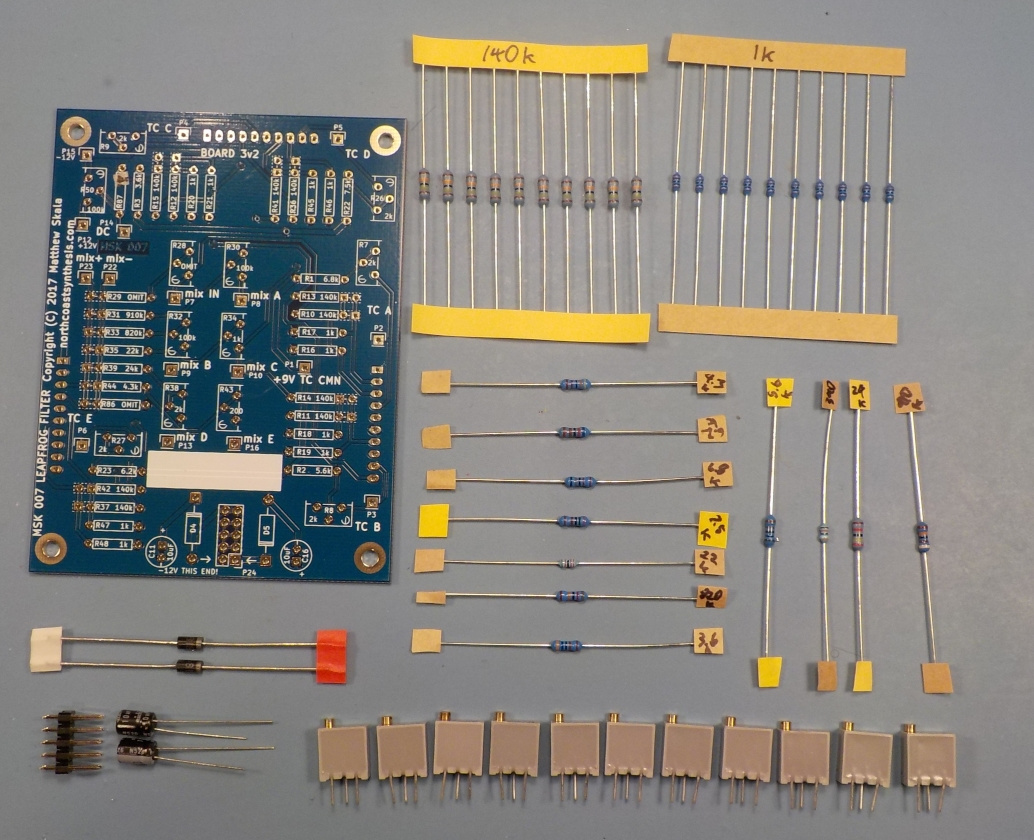
\includegraphics[width=\linewidth]{board3-parts.jpg}

There are 11 multiturn trimmers to be installed on this board.  Before
installing them, use an ohmmeter to adjust each one to 50\% of its range. 
Measure the resistance along the track, then measure the resistance from the
wiper to one end and adjust to make the wiper half the total track
resistance.  This need not be exact, but it will help with adjustment later,
by reducing issues with interaction among the different settings.  With all
trimmers pre-set to 50\%, the module should basically work even if it is not
at its best, whereas if many are installed at extreme values instead, then
you may have trouble getting it up and running enough to adjust it more
accurately.

\begin{table*}
{\centering
\fbox{This table is not a substitute for the text instructions.}
\vspace{\baselineskip}

\begin{tabular}{rp{1in}cp{3in}}
  \textbf{Qty} & \textbf{Ref} & \textbf{Value/Part No.} & \\ \hline
\input{bomdata-3.tex}
\end{tabular}\par}
\caption{Bill of Materials for Board~3.}\label{tab:b3bom}
\end{table*}

\section{Fixed resistors}

In order to allow as many options as possible for modified filter curves
using this same PCB design, many of the resistors on Board~3 have special
three-pin footprints, as shown below.  These are meant to offer the choice
of connecting a signal to the positive or negative input of an op amp or
OTA.

\noindent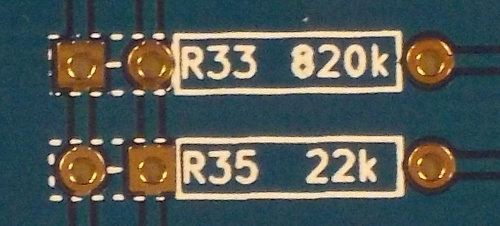
\includegraphics[width=\linewidth]{optres-empty.jpg}

In each of these special footprints the resistor connects between the pad at
right, and \emph{one of} the two pads at left.  The pad you should use for
the default response curve is always the pad with the \emph{square corners},
which may be the nearer or farther pad depending on the individual
footprint.  The other, circular, pad should not be used in a standard build
but is reserved for possible use by some future modification that may
require a different resistor network.

\noindent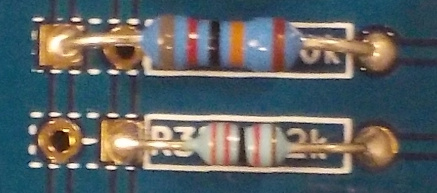
\includegraphics[width=\linewidth]{optres-filled.jpg}

Throughout the installation of the fixed resistors on Board~3, check
carefully against both the pad shapes on the board, and the photos in these
instructions, to be sure you install each resistor into the correct pads. 
Getting any wrong will likely result in little or no response from the
filter, or a highly distorted frequency response curve.

Resistors are never polarized.  I like to install mine in a consistent
direction for cosmetic reasons, but this is electrically unnecessary.  In
this module, metal film 1\%\ resistors are recommended for all fixed-value
resistors.  These will usually have blue bodies and four colour bands
designating the value, plus a fifth band for the tolerance, brown in the
case of 1\%.  These are the resistors normally shipped in the
North Coast kits, but we may occasionally ship better-tolerance resistors (such
as 0.5\%) if we are able to source them at a good price. 
Accordingly, I mention only the four value band colours for this type of
resistor; if you are using resistors with other codes, you are responsible
for knowing them.  Note that colour codes on metal film 1\% resistors are
often ambiguous (reading from one end or the other end may give two
different values, both plausible) and some of the colours are hard to
distinguish anyway.  If in doubt, always measure with an ohmmeter before
soldering the resistor in place.

Install the ten 1k$\Omega$ (brown-black-black-brown) resistors R16 through
R21 and R45 through R48.  These are parts of the voltage dividers
that control input levels for the five integrators making up the filter
core.  A full MSK~007 kit should contain 13 of these resistors, so there
should be three left over for use on the other boards.

\nopagebreak
\noindent\includegraphics[width=\linewidth]{{res-1.0k3}.jpg}

\newpage

Install the 3.6k$\Omega$ (orange-blue-black-brown) resistor R3.  This
resistor controls the linearizing diode current for integrator~C.

\nopagebreak
\noindent\includegraphics[width=\linewidth]{{res-3.6k3}.jpg}

Install the 4.3k$\Omega$ (yellow-orange-black-brown) resistor R44.  This
resistor controls the proportion of integrator~E in the output mix. 
Connect it to the nearer pad.  A full MSK~007 kit should contain two of
these resistors, so there should be one left over for use on Board~2.

\nopagebreak
\noindent\includegraphics[width=\linewidth]{{res-4.3k3}.jpg}

\newpage

Install the 5.6k$\Omega$ (green-blue-black-brown) resistor R2.  This
resistor controls the linearizing diode current for integrator~B.  A full
MSK~007 kit should contain seven of these resistors, so there should be six
left over for use on the other boards.

\nopagebreak
\noindent\includegraphics[width=\linewidth]{{res-5.6k3}.jpg}

Install the 6.2k$\Omega$ (blue-red-black-brown) resistor R23.  This resistor
controls the linearizing diode current for integrator~E.

\nopagebreak
\noindent\includegraphics[width=\linewidth]{{res-6.2k3}.jpg}

\newpage

Install the 6.8k$\Omega$ (blue-grey-black-brown) resistor R1.  This resistor
controls the linearizing diode current for integrator~A.

\nopagebreak
\noindent\includegraphics[width=\linewidth]{{res-6.8k3}.jpg}

Install the 7.5k$\Omega$ (violet-green-black-brown) resistor R22.  This
resistor controls the linearizing diode current for integrator~D.

\nopagebreak
\noindent\includegraphics[width=\linewidth]{{res-7.5k3}.jpg}

\newpage

Install the 22k$\Omega$ (red-red-black-red) resistor R35.  This resistor
controls the proportion of integrator~C in the output mix.  Connect it to
the nearer pad.  A full MSK~007 kit should contain two of these resistors,
so there should be one left over for use on Board~1.

\nopagebreak
\noindent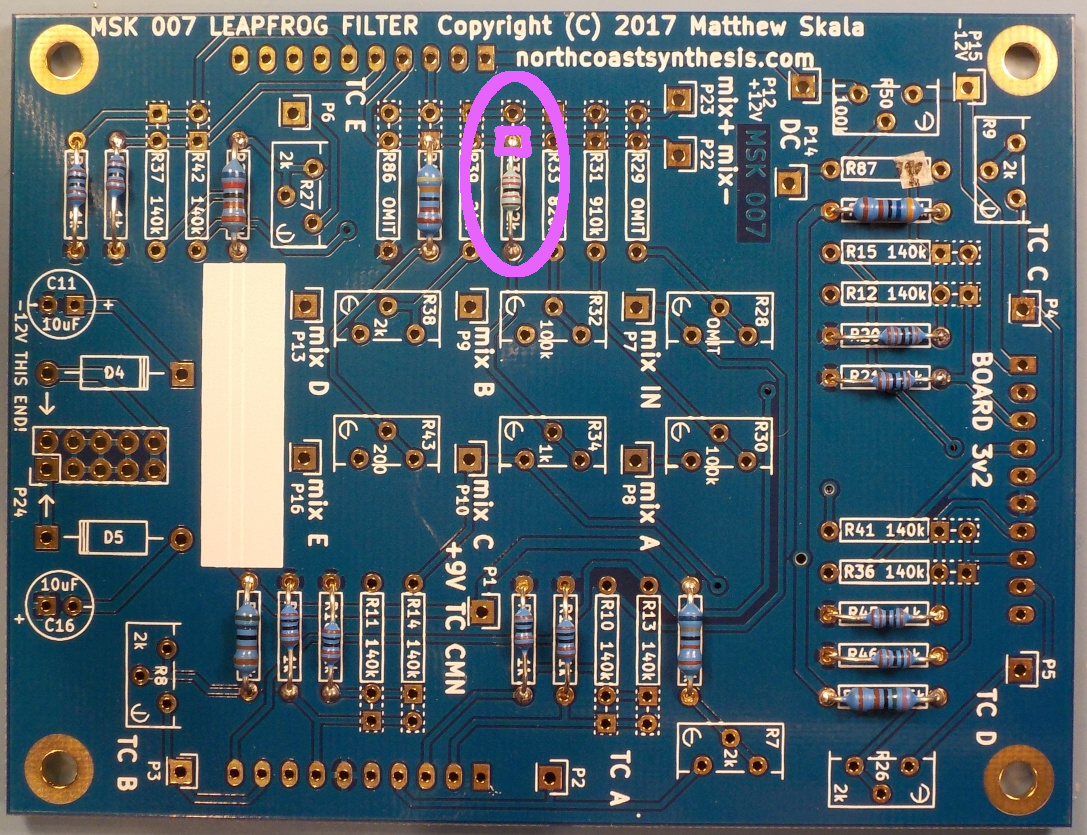
\includegraphics[width=\linewidth]{res-22k3.jpg}

Install the 24k$\Omega$ (red-yellow-black-red) resistor R39.  This resistor
controls the proportion of integrator~D in the output mix.  Connect it to
the farther pad.

\nopagebreak
\noindent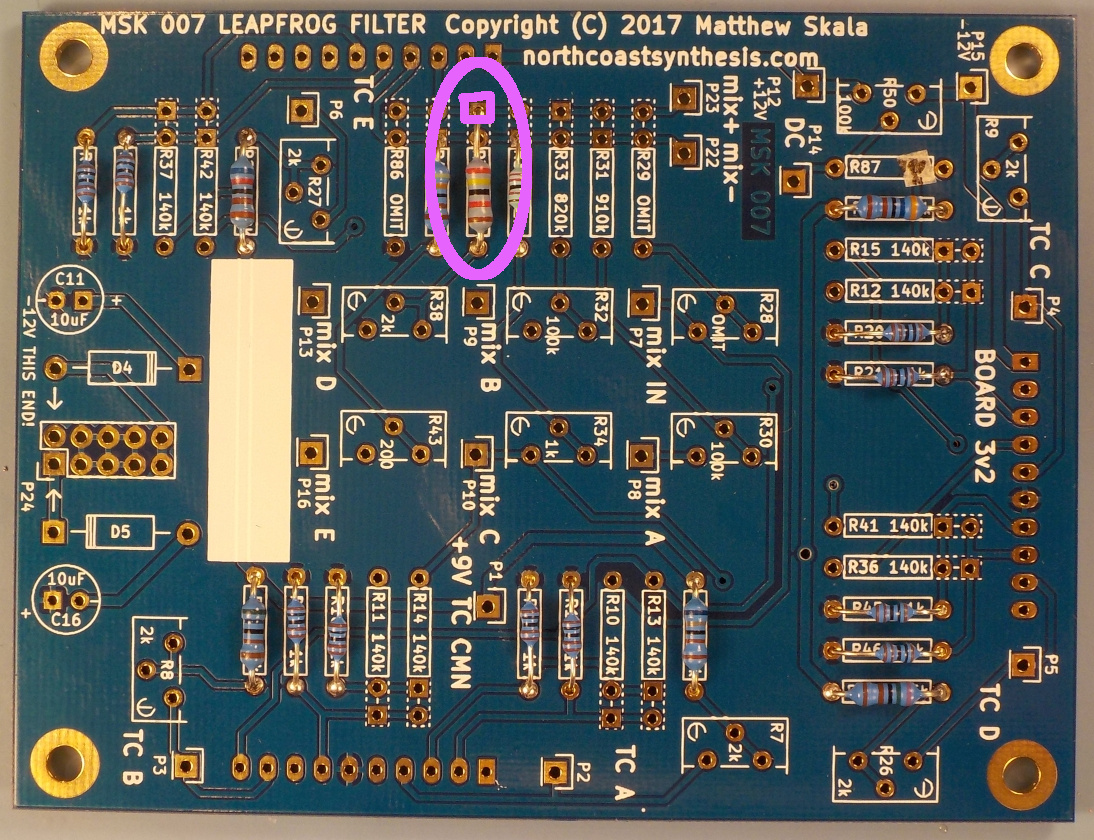
\includegraphics[width=\linewidth]{res-24k3.jpg}

\newpage

Install the ten 140k$\Omega$ (brown-yellow-black-orange) resistors R10
through R15, R36, R37, R41, and R42.  These are parts of the voltage
dividers that control input levels for the five integrators.  The resistors
are installed in five pairs, each with one connected to the nearer and one
connected to the farther pad.  Check the photo and the board pad shapes
carefully.  A full MSK~007 kit should contain 11 of these resistors, leaving
one for use on Board~2.

\nopagebreak
\noindent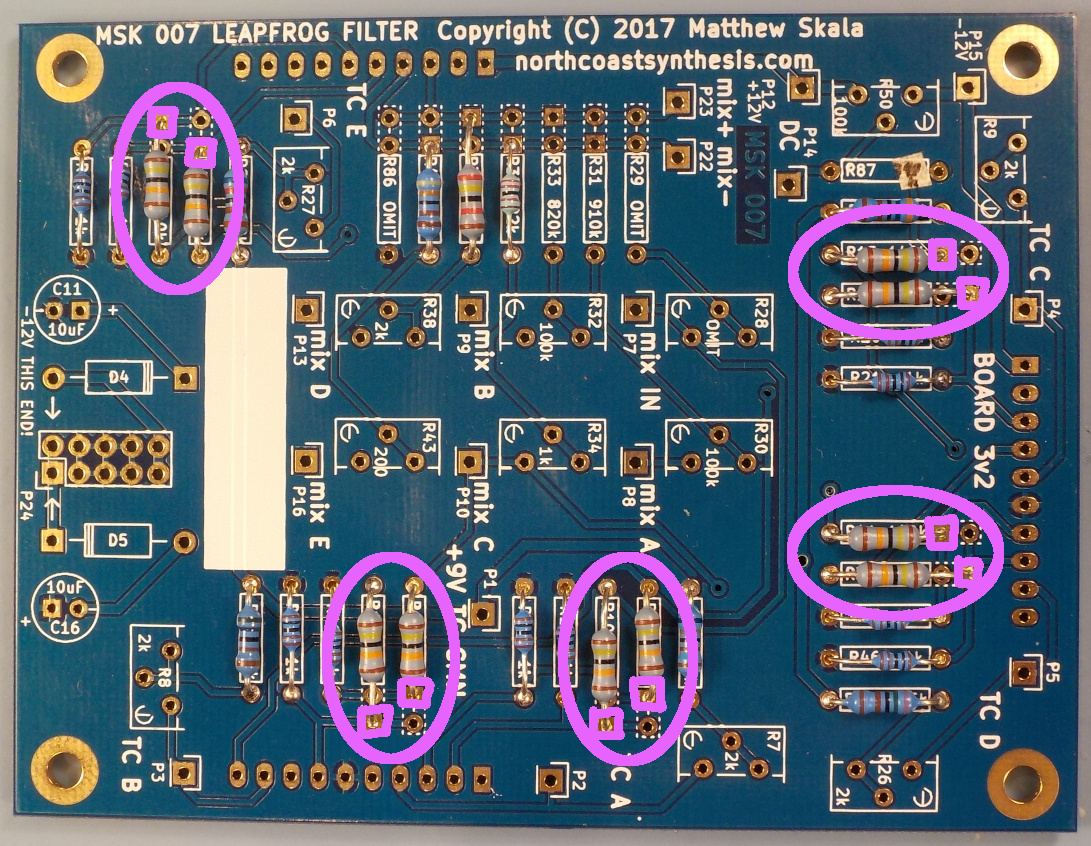
\includegraphics[width=\linewidth]{res-140k3.jpg}

Install the 390k$\Omega$ (orange-white-black-orange) resistor R87.  This
resistor sets the adjustment range for the core DC offset trimmer.  Note that
if you have a v2 board (like the one in the photo) then the silkscreen for
this resistor will read ``1M'' and possibly be covered by a bit of tape;
nonetheless, you should install a 390k$\Omega$ resistor here.

\nopagebreak
\noindent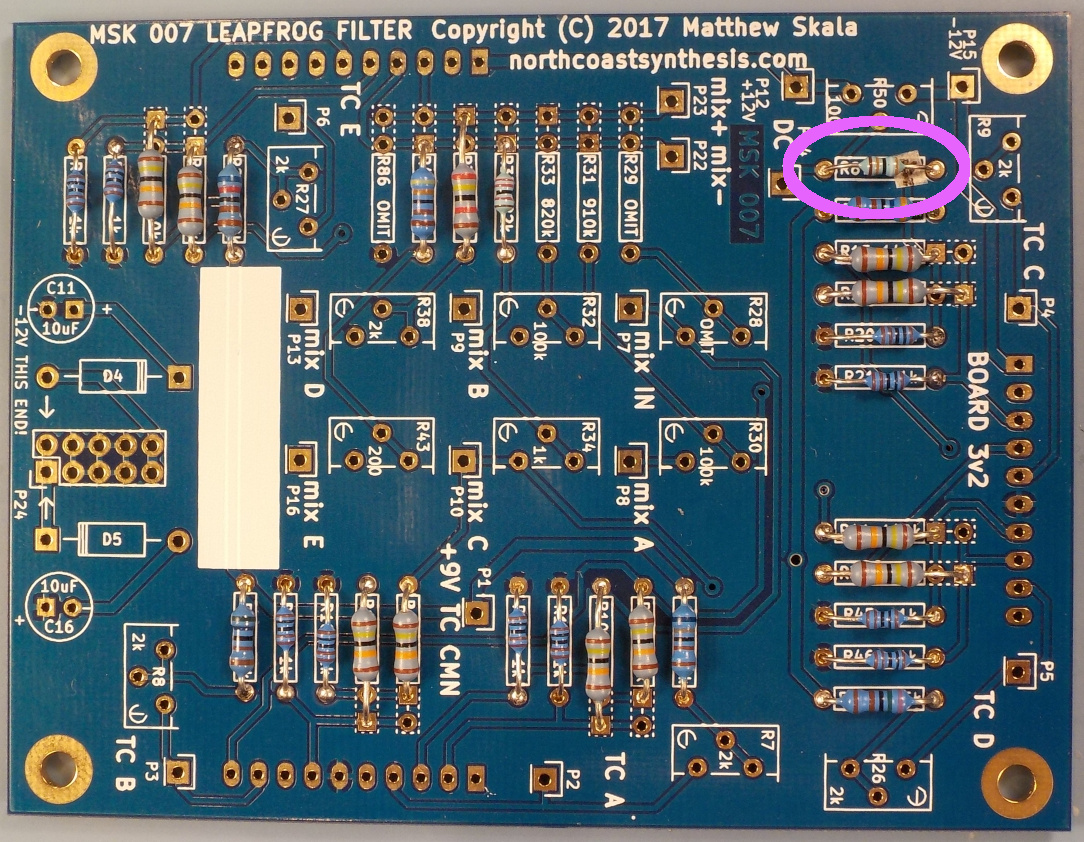
\includegraphics[width=\linewidth]{res-390k3.jpg}

\newpage

Install the 820k$\Omega$ (grey-red-black-orange) resistor R33.  This resistor
controls the proportion of integrator~B in the output mix.  Connect it to
the farther pad.

\nopagebreak
\noindent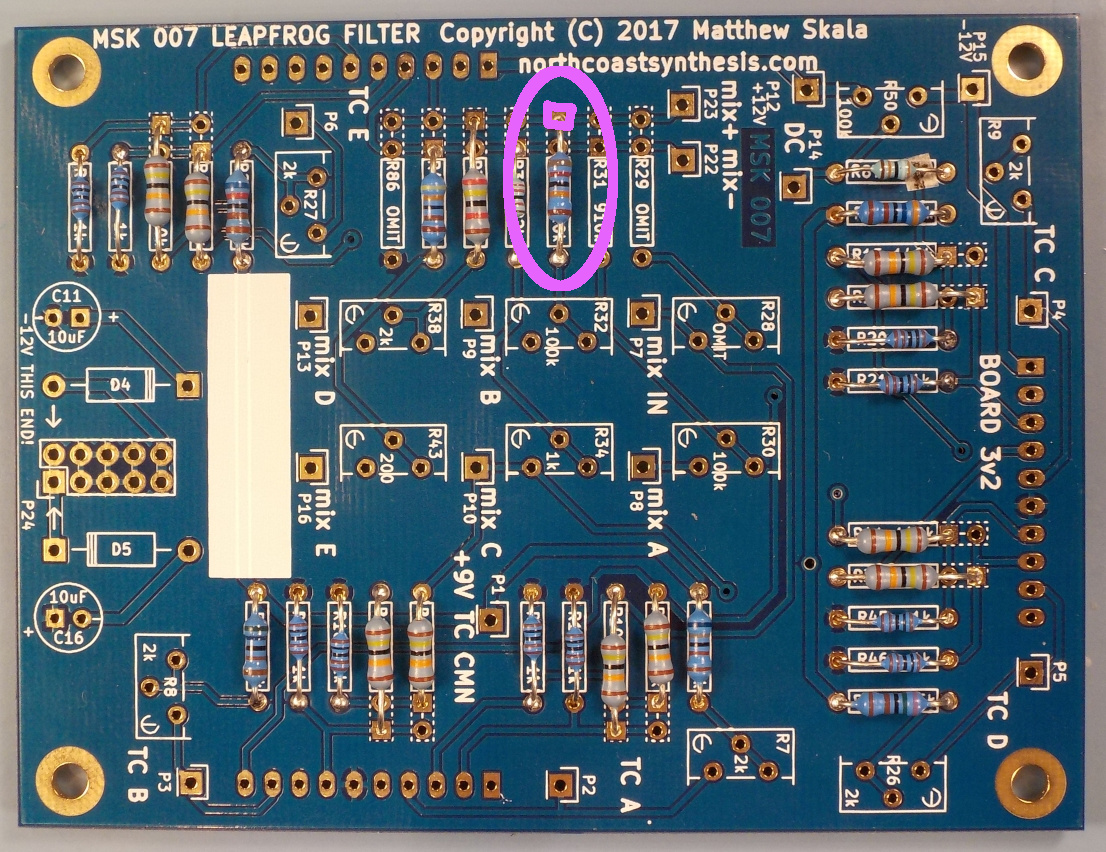
\includegraphics[width=\linewidth]{res-820k3.jpg}

Install the 910k$\Omega$ (white-brown-black-orange) resistor R31.  This
resistor controls the proportion of integrator~A in the output mix.  Connect
it to the nearer pad.

\nopagebreak
\noindent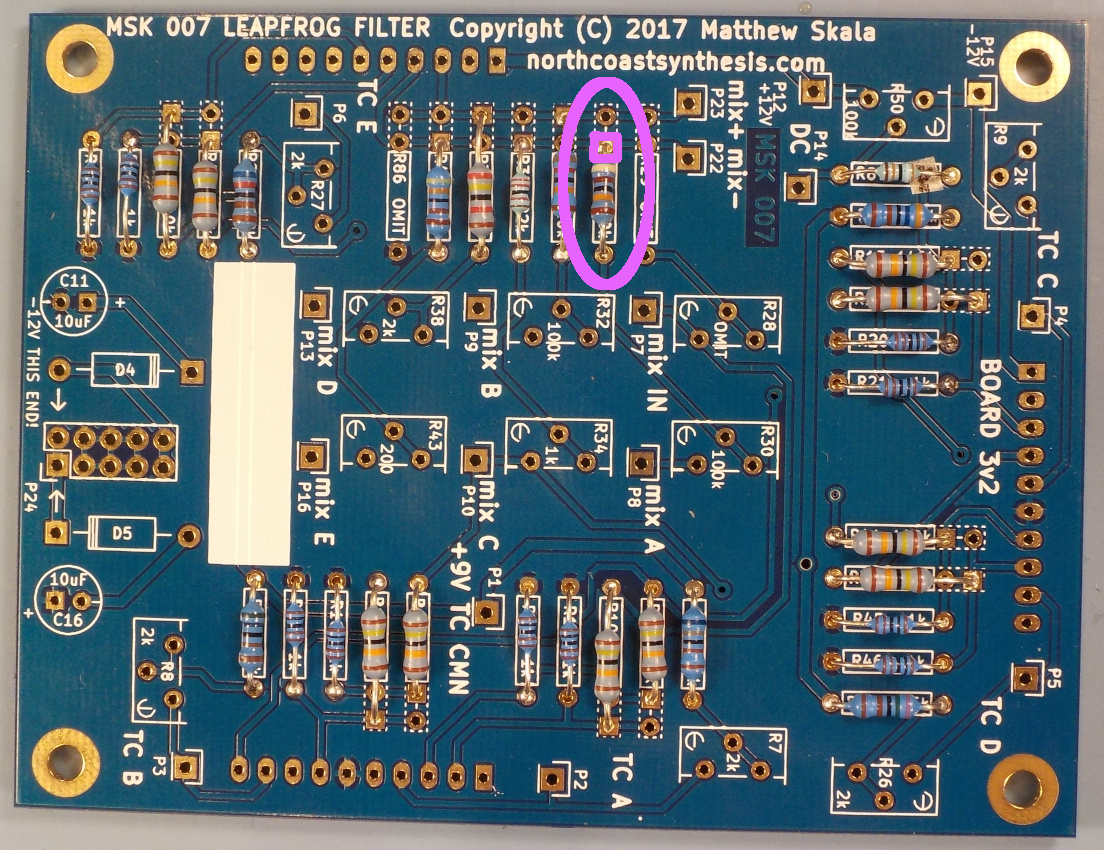
\includegraphics[width=\linewidth]{res-910k3.jpg}

\section{Semiconductors}

Install the two Schottky diodes D4 and D5.  These protect the module against
reverse connection of the power supply.  They are polarized and must be
installed in the correct direction; otherwise they will prevent the module
from operating.  One end of each diode will be marked, usually with a stripe
of grey paint around the black plastic body of the diode.  That end is the
cathode.  The diode outline on the PCB silkscreen is marked with a
similar stripe showing the direction of the cathode, and the solder pad for
the cathode is square instead of round.

\noindent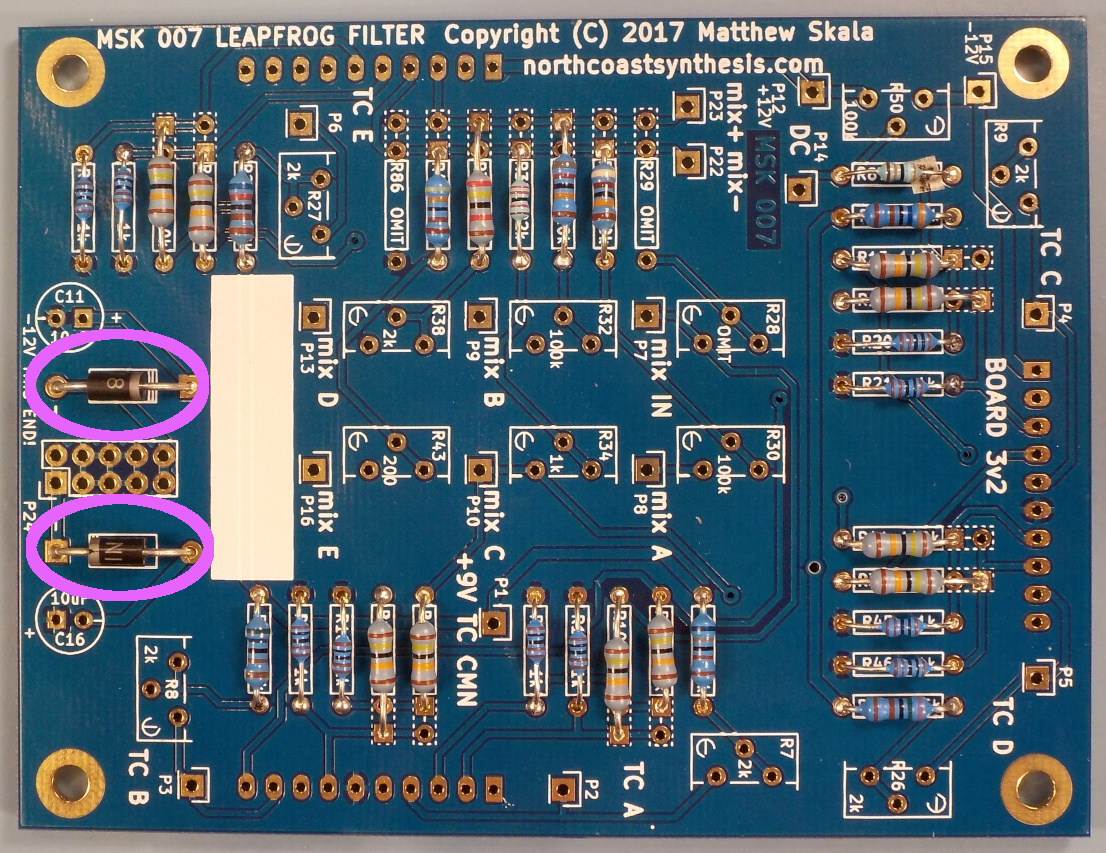
\includegraphics[width=\linewidth]{schottky.jpg}

\section{Electrolytic capacitors}

Install the two 10$\mu$F electrolytic capacitors C11 and C16.  These filter
incoming power to prevent noise in the case power system from affecting the
Leapfrog.  They are polarized components, and may explode if connected
backwards.  As such, there are multiple clues to help you install them in
the right direction.  The negative leg of each capacitor will be marked in
some way, usually with a printed stripe and minus signs on the plastic
wrapping of the capacitor body.  The negative leg of the capacitor will
usually also be shorter, though that is less reliable than the body
markings.  On the PCB, the positive and negative pads are marked with
positive and negative signs in the silkscreen, and the solder pads
themselves are round for negative and square for positive.

\noindent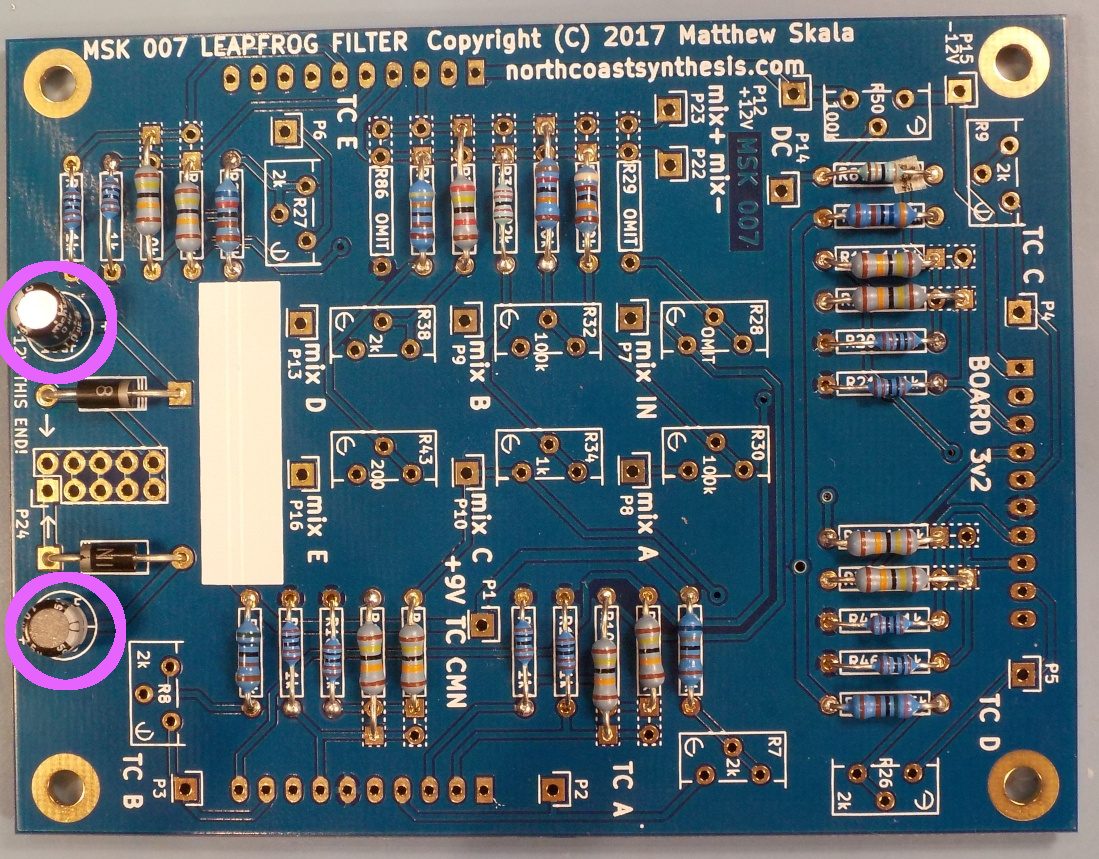
\includegraphics[width=\linewidth]{cap-10u3.jpg}

A full MSK~007 kit should contain four of these capacitors, leaving two
for installation on Board~2.

\section{Trimmer potentiometers}

If you have not already set the trimmers to 50\%\ of their full scale value
as described under ``Preliminaries'' above, then do it now.

Trimmers are not exactly polarized, but the three legs of each trimmer serve
different functions and need to be connected to the right holes.  The
physical arrangement of the legs and corresponding holes should make it
impossible to install the trimmers wrong way round.

Install the 200$\Omega$ trimmer R43.  This trimmer sets the proportion of
integrator~E in the output mix.

\nopagebreak
\noindent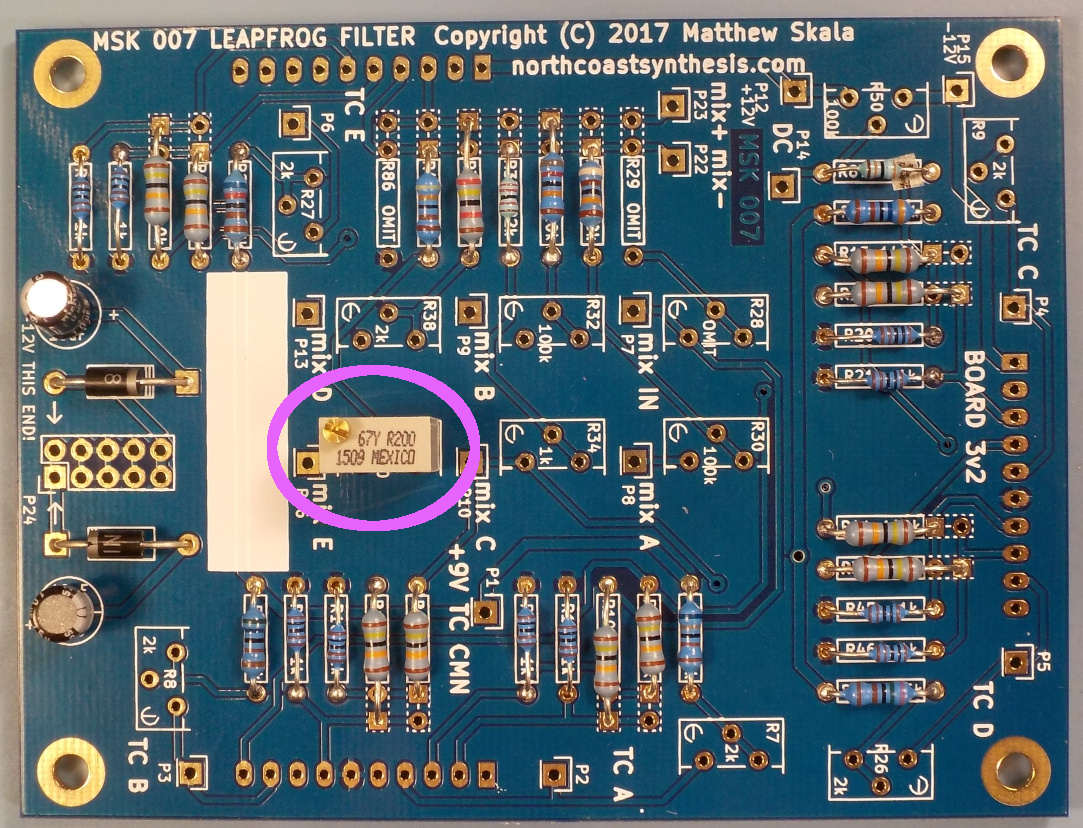
\includegraphics[width=\linewidth]{pot-200w3.jpg}

Install the 1k$\Omega$ trimmer R35.  This trimmer sets the proportion of
integrator~C in the output mix.

\nopagebreak
\noindent\includegraphics[width=\linewidth]{{pot-1.0k3}.jpg}

\newpage

Install the six 2k$\Omega$ trimmers R7 to R9, R26, R27, and R38.  Most of
these are for adjusting the diode currents, and indirectly the time
constants, of the integrator stages; R38 sets the proportion of integrator~D
in the output mix.

\nopagebreak
\noindent\includegraphics[width=\linewidth]{{pot-2.0k3}.jpg}

Install the three 100k$\Omega$ trimmers R30, R32, and R50.  The first two of
these set the output mix amounts for integrators~A and~B respectively; R50
is for adjusting the filter core DC offset.

\nopagebreak
\noindent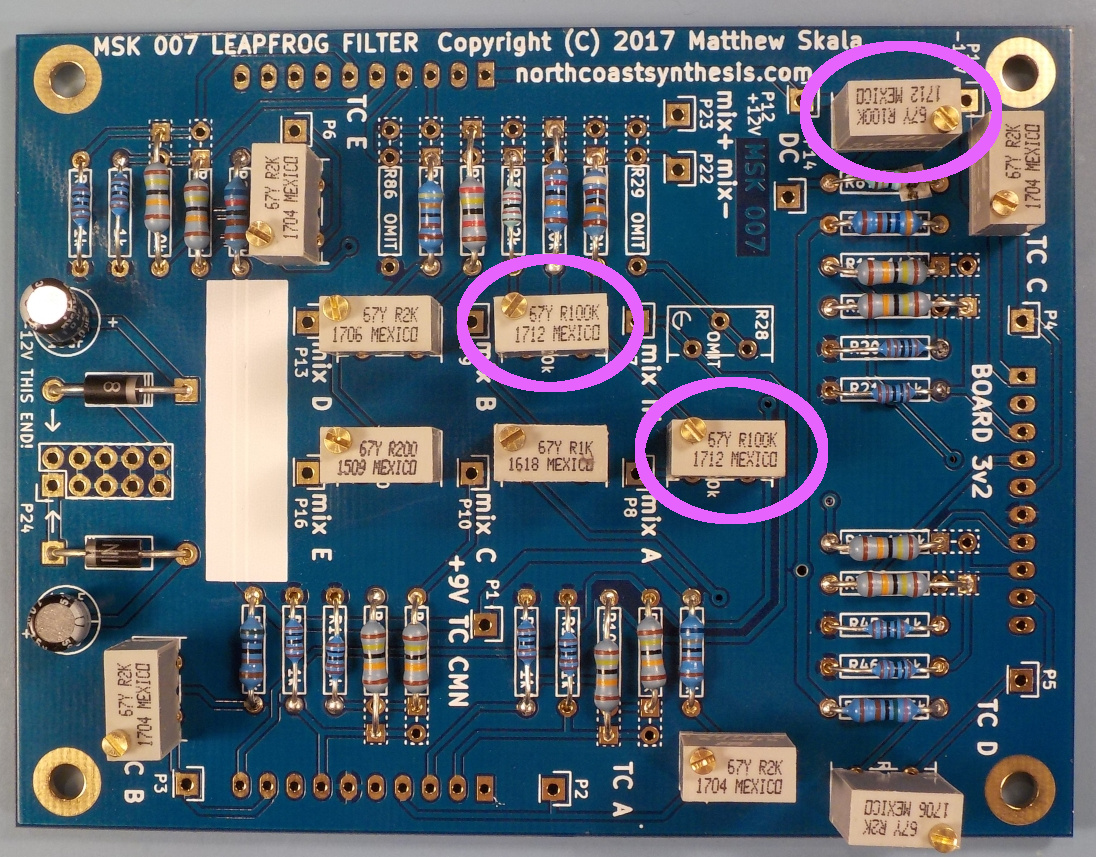
\includegraphics[width=\linewidth]{pot-100k3.jpg}

\section{Power header}

Install the 10-pin dual-row Eurorack power header P24.  It is not polarized
in the horizontal plane.  However, if it has shorter legs on one side, then
those are the ones that should go through the PCB (leaving the longer legs
sticking up to mate with the connector on the power cable), and if it has
tin plating on one end of the pins and gold on the other, then the tin side
should be the one soldered through the board.  Secure the header carefully
to the board, possibly with tape, before soldering it.  It is easy to
accidentally solder it at an angle, which is a difficult error to fix and
may cause trouble when you later attach the power cable.

\noindent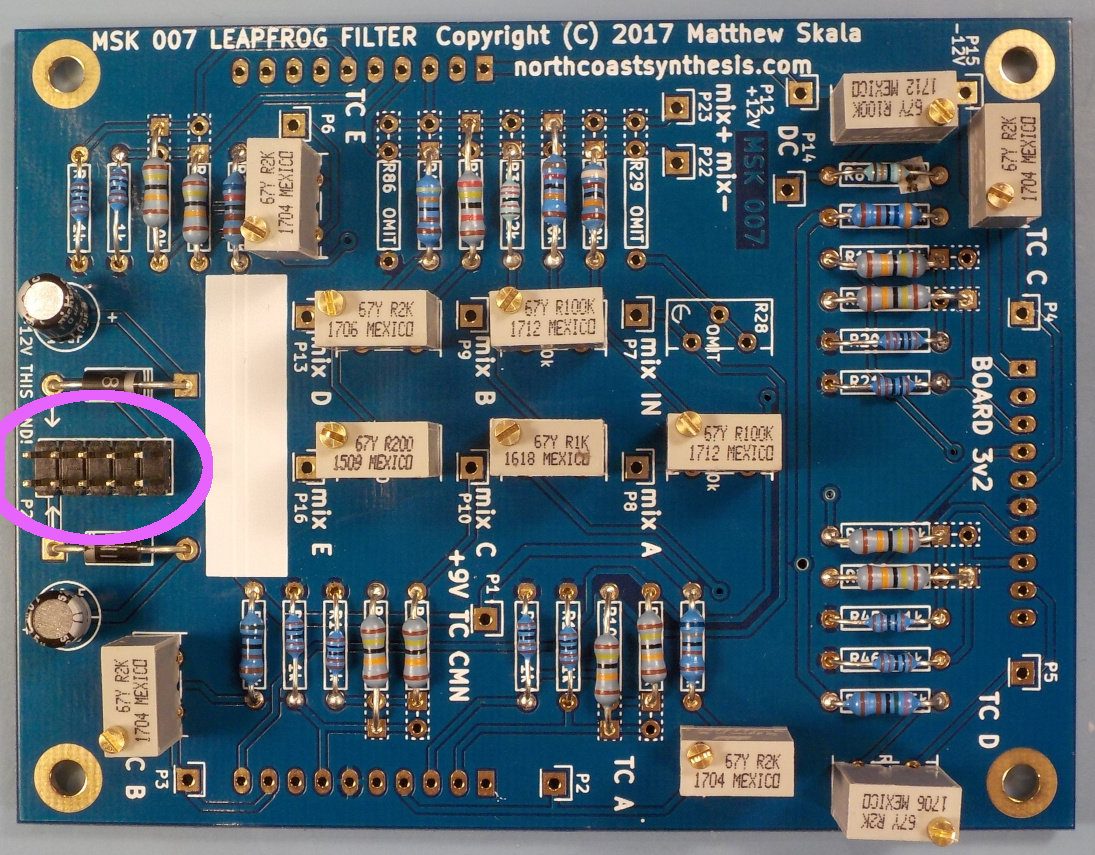
\includegraphics[width=\linewidth]{power.jpg}

Note that Eurorack power connections are polarized even if the connectors
are not.  The cables are usually grey ribbon type with a red stripe along
one side indicating pin 1, which carries $-$12V power.  For most modules
including the MSK~007, the red stripe should be at the \emph{bottom} when
the module is mounted vertically in a case.  On the MSK~007, the correct
location of the $-$12V supply is also marked with the text ``$-$12V THIS
END!'' and arrows on both sides of the PCB silkscreen.  This module is
also protected (by the Schottky diodes you just installed) from damage in
case of a reversed power connection; if you connect the power backwards and
nothing else is wrong, then the module will not power up but will be fine
once you connect the power correctly.  However, many other modules are not
so protected, and it is dangerous to get into the habit of depending on
protection diodes.  Destroying a module by connecting power backwards is
almost a rite of passage for Eurorack users.

At this point you may, if you wish, do the pre-adjustment procedure
described starting on page~\pageref{ch:preadj}.  Whether you do that now or
leave it until the rest of the build is complete, in between completed
boards is a good time to take a break.

% $Id: board2.tex 9464 2021-10-14 16:51:12Z mskala $

%
% MSK 009 Board 2 build instructions
% Copyright (C) 2018  Matthew Skala
%
% This program is free software: you can redistribute it and/or modify
% it under the terms of the GNU General Public License as published by
% the Free Software Foundation, version 3.
%
% This program is distributed in the hope that it will be useful,
% but WITHOUT ANY WARRANTY; without even the implied warranty of
% MERCHANTABILITY or FITNESS FOR A PARTICULAR PURPOSE.  See the
% GNU General Public License for more details.
%
% You should have received a copy of the GNU General Public License
% along with this program.  If not, see <http://www.gnu.org/licenses/>.
%
% Matthew Skala
% https://northcoastsynthesis.com/
% mskala@northcoastsynthesis.com
%

\chapter{Building Board 2}

The recommended order for building this module is to assemble Board 2, the
one further from the front panel, first.  That will make it easier to get
all the physical positioning right for the components that bridge between
the boards or pass through the panel.

Note that although I'm describing a separate step for each component value,
and that's how I built my prototype so as to have plenty of photo
opportunities, if you are reasonably confident about your skills you may
find it easier to populate all or most of the board (i.e.\ put the
components in place) and then solder them in a single step.  Except where
noted, the order in which you add components does not matter much.

\section{Preliminaries}

Count out the right number of everything according to the bill of materials. 
There is an abbreviated BOM for Board~2, excluding a few items that will be
added when combining this board with Board~1, in Table~\ref{tab:b2bom}.

\nopagebreak
\noindent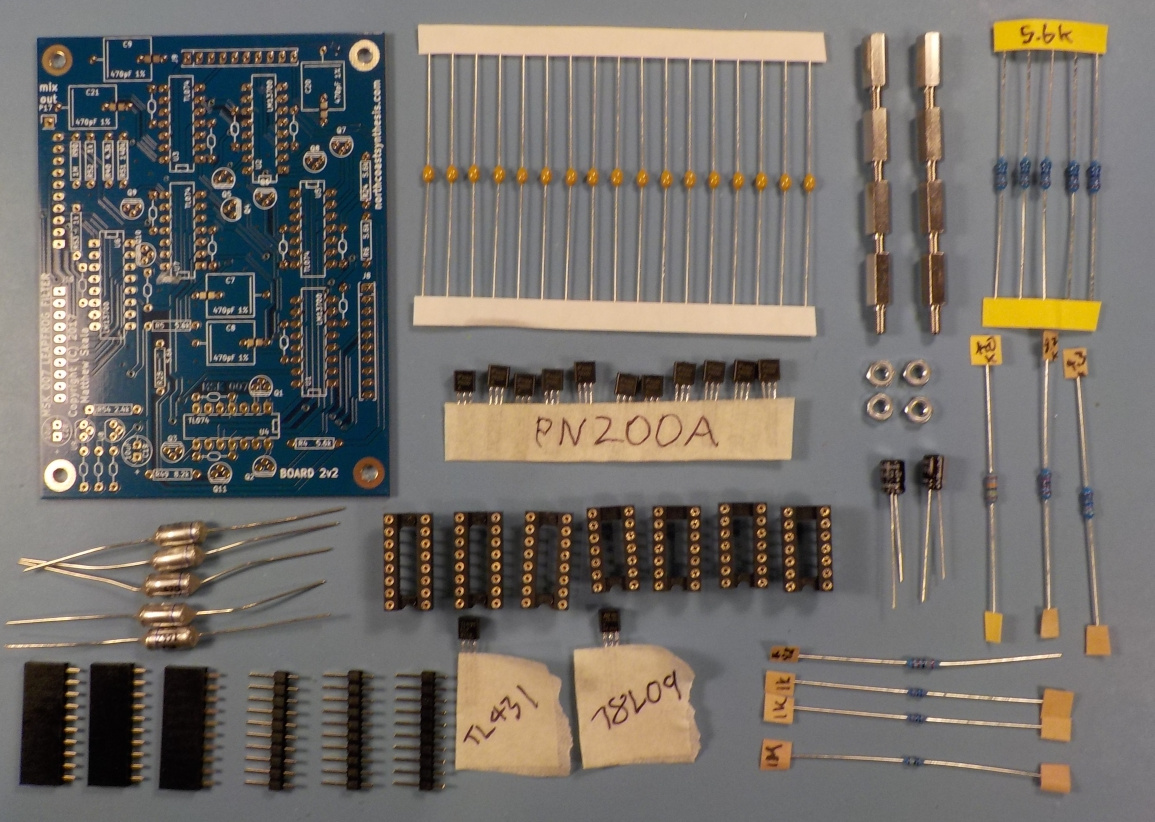
\includegraphics[width=\linewidth]{board2-parts.jpg}

There are two trimmers to be installed on this board.  Before
installing them, use an ohmmeter to adjust each one to 50\% of its range. 
Measure the resistance along the track, then measure the resistance from the
wiper to one end and adjust to make the wiper half the total track
resistance.  This need not be exact, but having them start near their
midpoints will help with adjustment later,
by reducing issues with interaction among the different settings.  With both
trimmers pre-set to 50\%, the module should basically work even if it is not
at its best, whereas if they are installed at extreme values instead, then
you may have trouble getting it up and running enough to adjust it more
accurately.

\begin{table*}
{\centering
\fbox{This table is not a substitute for the text instructions.}
\vspace{\baselineskip}

\begin{tabular}{rp{1.3in}cp{3in}}
  \textbf{Qty} & \textbf{Ref} & \textbf{Value/Part No.} & \\ \hline
\input{bomdata-2.tex}
\end{tabular}\par}
\caption{Bill of Materials for assembling Board~2.  Also needed is the PCB
itself.}\label{tab:b2bom}
\end{table*}

\section{Decoupling capacitors}

The four axial ceramic 0.1$\mu$F decoupling capacitors, C8 to C11, are shown
on the board by a special symbol without their reference designators.

\nopagebreak
\noindent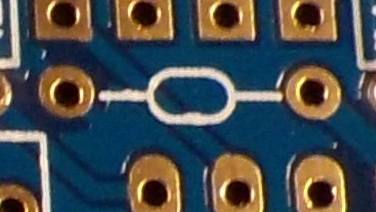
\includegraphics[width=\linewidth]{decoup-symbol.jpg}

Install these four capacitors where the symbol appears.  They are not
polarized and may be installed in either orientation.  These capacitors act
as filters for the power supplies to the op amp and OTA chips.  An MSK~009
kit should include six of these capacitors, and only four are used on this
board; save the remaining two for use on Board~1.

\nopagebreak
\noindent\includegraphics[width=\linewidth]{{cap-0.1u2}.jpg}

\section{Fixed resistors}

Resistors are never polarized.  I like to install mine in a consistent
direction for cosmetic reasons, but this is electrically unnecessary.  In
this module, the fixed resistors are metal film 1\%\ type.  They usually
have blue bodies and four colour bands designating the value, plus a fifth
band for the tolerance.  The tolerance band is brown for 1\%, but note that
we may occasionally ship better-tolerance resistors in the kits than the
specifications require, if we are able to source them at a good price. 
Accordingly, I mention only the four value band colours for this type of
resistor; if you are using resistors with other codes, you are responsible
for knowing them.  Note that colour codes on metal film 1\% resistors are
often ambiguous (reading from one end or the other end may give two
different values, both plausible) and some of the colours are hard to
distinguish anyway.  If in doubt, always measure with an ohmmeter before
soldering the resistor in place.

Install the four 510$\Omega$ (green-brown-black-black) resistors R22, R23,
R32, and R33.  These resistors, with the 100k$\Omega$ ones added later, set
the signal levels at the inputs of the OTA chips.

\nopagebreak
\noindent\includegraphics[width=\linewidth]{{res-510}.jpg}

\pagebreak
Install the two 9.1k$\Omega$ (white-brown-black-brown) resistors R24 and
R34.  These limit the maximum control current for the OTAs.

\nopagebreak
\noindent\includegraphics[width=\linewidth]{{res-9.1k}.jpg}

Install the two 10k$\Omega$ (brown-black-black-red) resistors R25 and R35. 
These are feedback resistors for the current-to-voltage converters in the
filter core.

\nopagebreak
\noindent\includegraphics[width=\linewidth]{{res-10k}.jpg}

\pagebreak
Install the four 27k$\Omega$ (red-violet-black-red) resistors R21, R26, R31, and R36. 
These are feedback resistors for the integrators (R26 and R36), and set the
current for the linearizing diodes in the LM13700 chips (R1 and R31).

\nopagebreak
\noindent\includegraphics[width=\linewidth]{{res-27k}.jpg}

Install the two 100k$\Omega$ (brown-black-black-orange) resistors R18 and
R28.  These resistors participate in setting the input levels for the OTA
chips.  A full kit contains seven resistors of this value; five should
remain for use on Board~1.

\nopagebreak
\noindent\includegraphics[width=\linewidth]{{res-100k2}.jpg}

Install the two 220k$\Omega$ (red-red-black-orange) resistors R19 and
R29.  These resistors set the adjustment ranges for the DC offset trimmers.
A full kit contains four
resistors of this value; save two for use on Board~1.

\nopagebreak
\noindent\includegraphics[width=\linewidth]{{res-220k2}.jpg}

\section{Semiconductors}

Install the two 1N5818 or SBA130 Schottky rectifier diodes D2 and D3.  These
are for reverse-voltage protection; they cut off power to the module when
the power plug is backwards.  They are polarized and it is important to
install them in the right direction.  Each diode is packaged inside a black
or dark grey plastic slug with a white or light grey stripe at one end; that
end is the \emph{cathode}.  The silkscreen markings on the board have a
corresponding stripe and the diodes should be installed with their stripes
matching the markings on the board.  The solder pads for the cathodes are
also square instead of round.  Installing these backwards means they will
have the opposite of the intended protective effect.

\nopagebreak
\noindent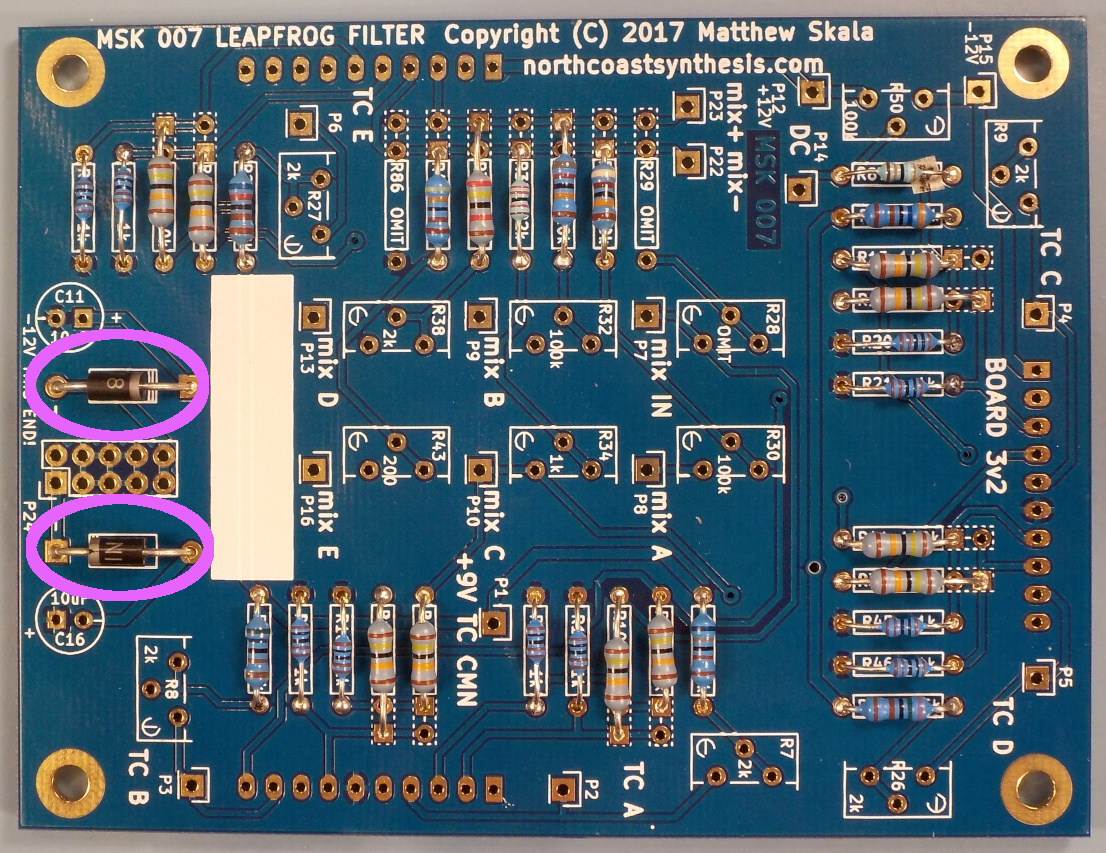
\includegraphics[width=\linewidth]{schottky.jpg}

Install the 14-pin DIP socket for the operational amplifier chip U2.  This
chip does most of the amplification in the filter core.  DIP sockets
themselves do not care which direction you install them, but it is
critically important that the chips installed in the sockets should be
installed in the right direction.  To help with that, the sockets will
probably be marked with notches at one end (indicating the end where Pin~1
and Pin~14 are located) and you should install the sockets so that the
notched ends match the notches shown on the PCB silkscreen.  The solder pad
for Pin~1 is also distinguished by being rectangular instead of rounded.

Installing DIP sockets without having them tilted at a funny angle can be
tricky.  I recommend inserting the socket in the board, taping it in place
on the component side with vinyl electrical tape or sticking it there with a
small blob of putty at each end, then soldering one pin on
one corner and checking that the socket is snug against the board before
soldering the other pins.  That way, if you accidentally solder the first
pin with the socket tilted, it will be easier to correct (only one pin to
desolder instead of all of them).

\nopagebreak
\noindent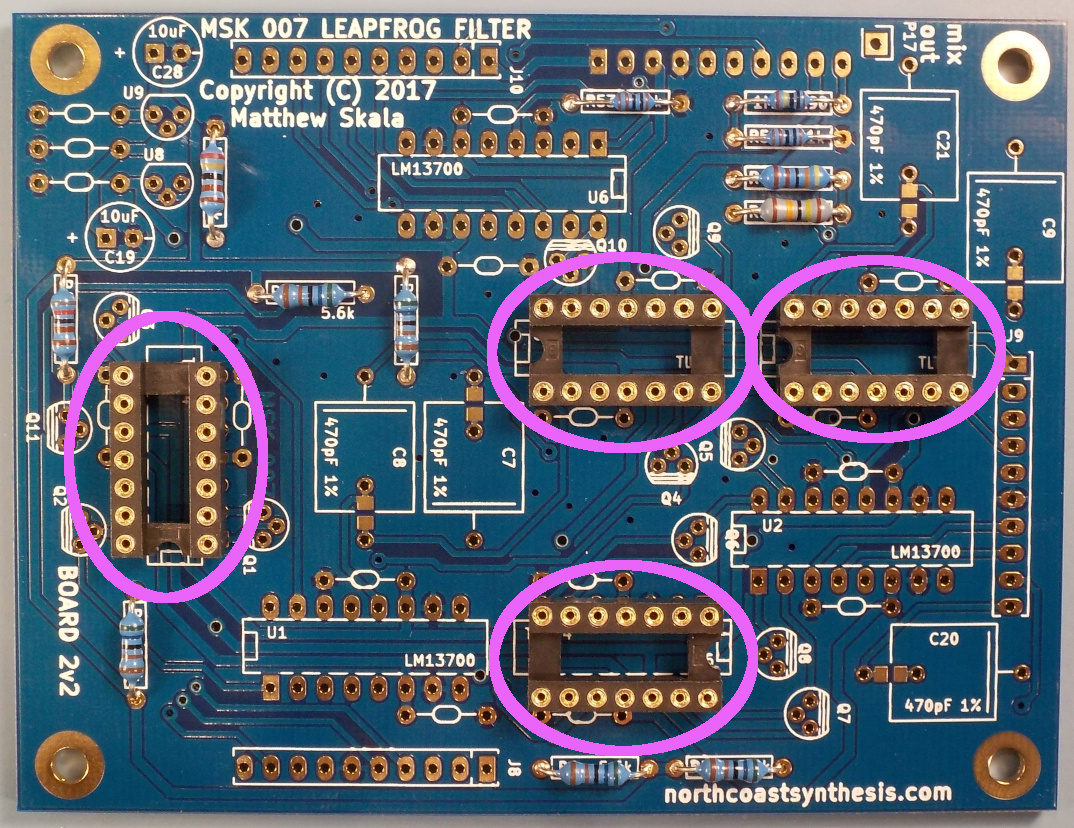
\includegraphics[width=\linewidth]{dip14-2.jpg}

If you somehow manage to solder an entire socket in backwards, don't try to
desolder it to turn it around.  Just leave it as it is and remember that
when you insert the chip, you must insert it so the chip matches the
markings on the \emph{board}, not the turned-around socket.

Install the 16-pin DIP socket for the OTA (operational transconductance
amplifier) chip U3.  This chip contains two current-controlled amplifiers,
which, by means of a frequency-dependent control current, tune the filter
core to the desired frequency.  See the general instructions regarding DIP
sockets above.

\nopagebreak
\noindent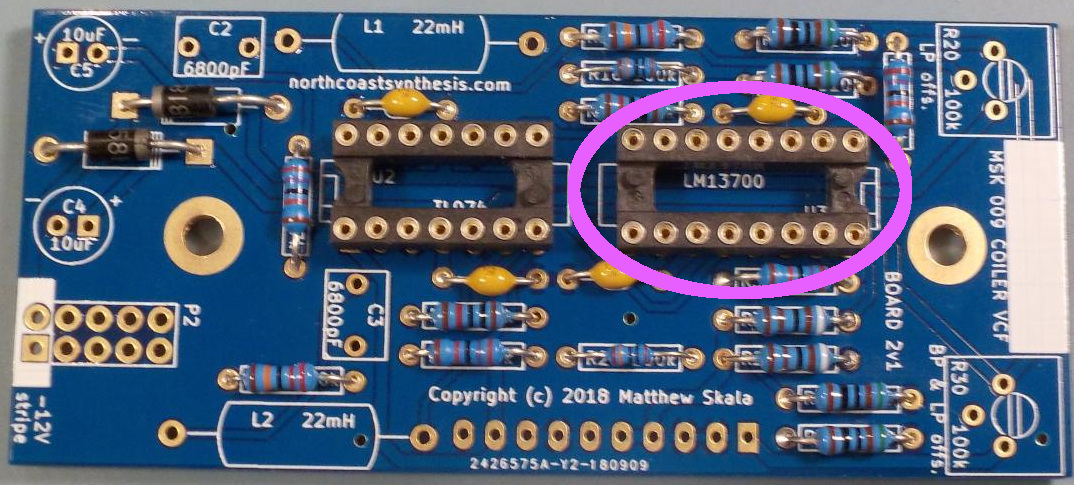
\includegraphics[width=\linewidth]{dip16.jpg}

\section{Electrolytic and film capacitors}

Install the two 6800pF film capacitors C2 and C3.  These are timing
components used in the integrators at low frequencies to complement the
inductors used at medium to high frequencies.  They are unpolarized
components and may be installed in either orientation.

The markings on film capacitors may vary depending on the manufacturer and
model.  These ones might be marked ``682'' (for 68 followed by two 0s number
of picofarads), ``6n8'' (for 6.8nF), or even ``0.0068'' (value in $\mu$F). 
However, these are the only film capacitors in the module, so confusion is
unlikely.

\nopagebreak
\noindent\includegraphics[width=\linewidth]{{cap-6800p}.jpg}

\pagebreak

Install the two 10$\mu$F electrolytic capacitors C4 and C5, which
filter the power supply for the module as a whole. 
These are polarized components and they may explode if installed backwards. 
Each one will be marked on its casing with a stripe and minus signs to
indicate the negative lead; the positive lead will probably also be longer. 
These clues should be matched with the markings on the PCB: plus and minus
symbols in the silkscreen and a square solder pad for the positive (long)
lead.

\nopagebreak
\noindent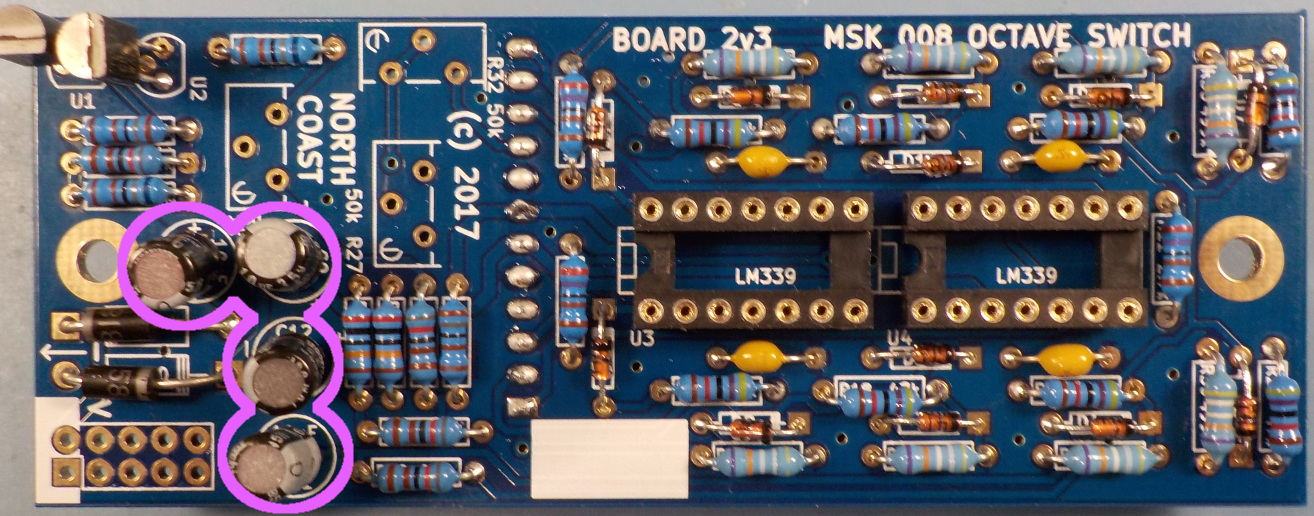
\includegraphics[width=\linewidth]{cap-10u.jpg}

\section{Trimmer potentiometers}

If you have not already set the trimmers to 50\%\ of their full scale value
as described under ``Preliminaries'' above, then do it now.

Trimmers usually are not washable, so if you plan to clean your boards by
full immersion in water or other solvent,
your last chance is now; future cleaning will have to
be done with a brush and some care to avoid letting liquid seep into the
trimmers.  Even now you should take some care with the DIP sockets, because
solvent can carry flux residue into them and form a varnish-like layer if
not carefully rinsed away.

Trimmers are not exactly polarized, but the three legs of each trimmer serve
different functions and need to be connected to the right holes.  The
physical arrangement of the legs and corresponding holes should make it
impossible to install the trimmers wrong way round.

Install the two 100k$\Omega$ trimmers R20 and R30.  These trimmers
are for compensating DC offsets in the filter core.

\nopagebreak
\noindent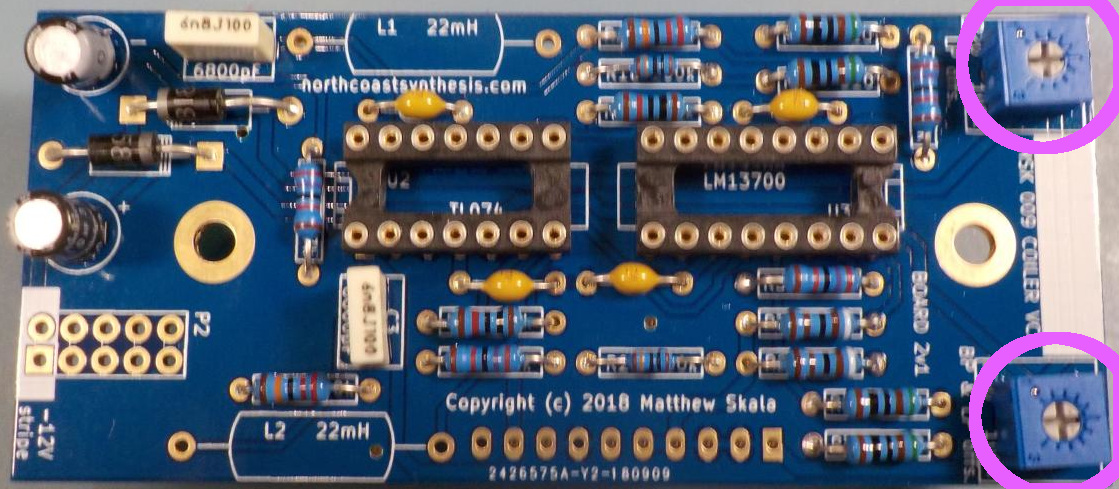
\includegraphics[width=\linewidth]{pot-100k2.jpg}

\pagebreak

\section{Inductors}

The two 22mH ferrite-bobbin inductors, that is, \emph{coils}, L1 and L2 give
this module its name.  Install them now.  They are the main timing
components in the filter core, serving at medium to high frequencies. 
Single inductors like these have no polarity and may be installed in either
direction; the situation is more complicated with transformers made of two
or more interacting inductors.

The inductors are delicate, especially in the area where the leads attach to
the bodies, because the windings that connect to the leads are made of very
fine wire.  The ferrite core material is also somewhat brittile.  It is
important not to bend the leads too close to the bodies.  There is some
extra space for the inductors on the circuit board to allow for a gentle
bend radius.

\nopagebreak
\noindent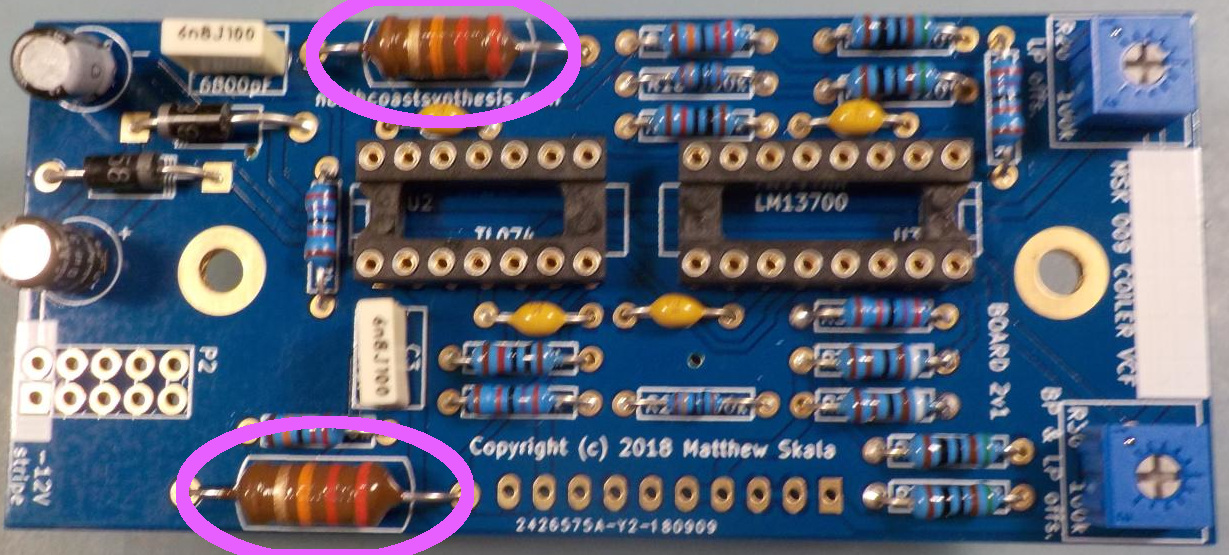
\includegraphics[width=\linewidth]{coils.jpg}

\section{Eurorack power connector}

Install the 2$\times$5-pin Eurorack power connector J2.  This connector is
not polarized in itself, although the connection it makes is polarized.  As
with the DIP sockets, you should be careful to get it installed snugly
against the board, not tilted at an angle.  Use tape or putty to
hold it in place, solder one pin, then check that it is straight before you
solder the other pins.

The six pins in the centre of the connector, that is all except the four
corner pins, are for grounding and they are all connected together on the
board.  Thus, if you accidentally form solder bridges among these six pins
while installing the connector, don't waste effort trying to remove them;
they will have no electrical effect.

\nopagebreak
\noindent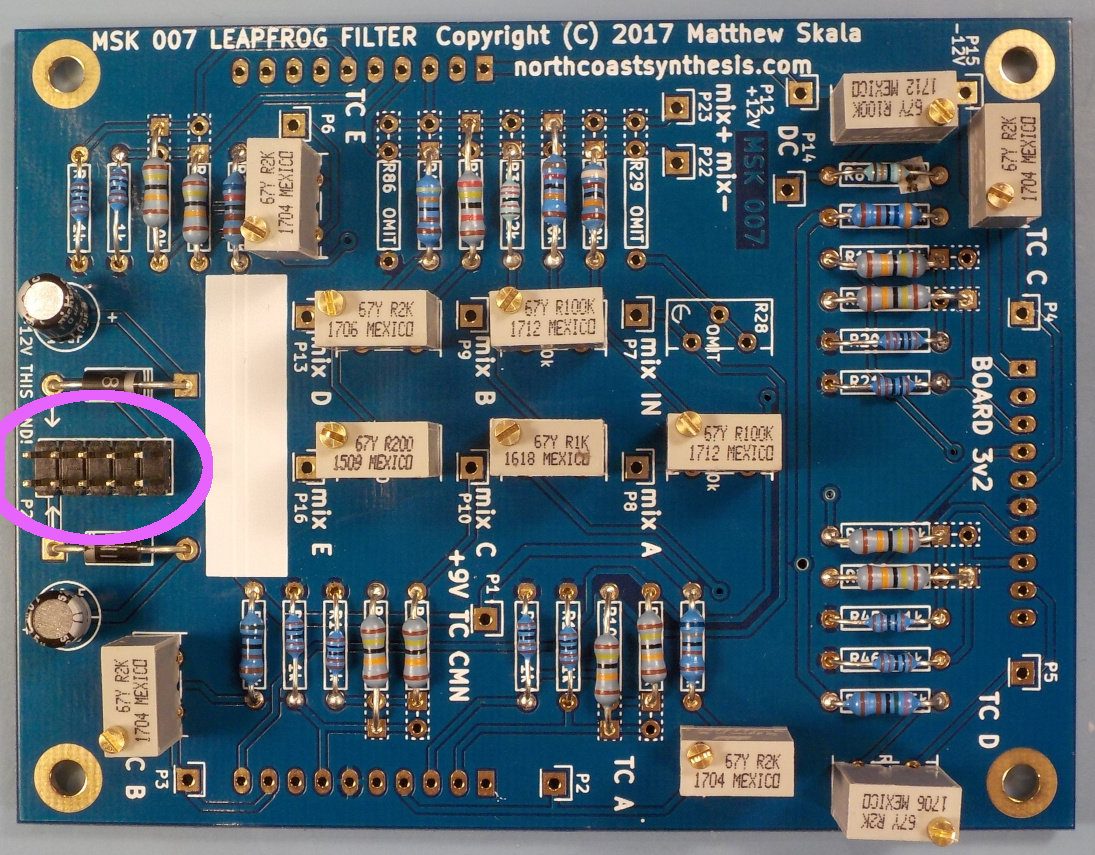
\includegraphics[width=\linewidth]{power.jpg}

In between completed boards is a good time to take a break.


% $Id: board1.tex 9375 2021-08-31 13:01:06Z mskala $

%
% MSK 007 Board 1 build instructions
% Copyright (C) 2017, 2020, 2021  Matthew Skala
%
% This program is free software: you can redistribute it and/or modify
% it under the terms of the GNU General Public License as published by
% the Free Software Foundation, version 3.
%
% This program is distributed in the hope that it will be useful,
% but WITHOUT ANY WARRANTY; without even the implied warranty of
% MERCHANTABILITY or FITNESS FOR A PARTICULAR PURPOSE.  See the
% GNU General Public License for more details.
%
% You should have received a copy of the GNU General Public License
% along with this program.  If not, see <http://www.gnu.org/licenses/>.
%
% Matthew Skala
% https://northcoastsynthesis.com/
% mskala@northcoastsynthesis.com
%

\chapter{Building Board 1}

Board~1 has components on both sides, which makes the order of assembly
important; installing the wrong components first may make it difficult to
safely maneuver the soldering iron to install later components without
damaging the already-installed components.  This chapter also includes
instructions on installing the connector on Board~2 that links it to
Board~1.

\section{Preliminaries}

Count out the right number of everything according to the bill of materials. 
There is an abbreviated BOM for Board~1, and the final assembly steps, in
Table~\ref{tab:b1bom}.  In addition to these things you will need your
assembled Boards~2 and~3 from the previous chapters, and the hardware
associated with them.

\noindent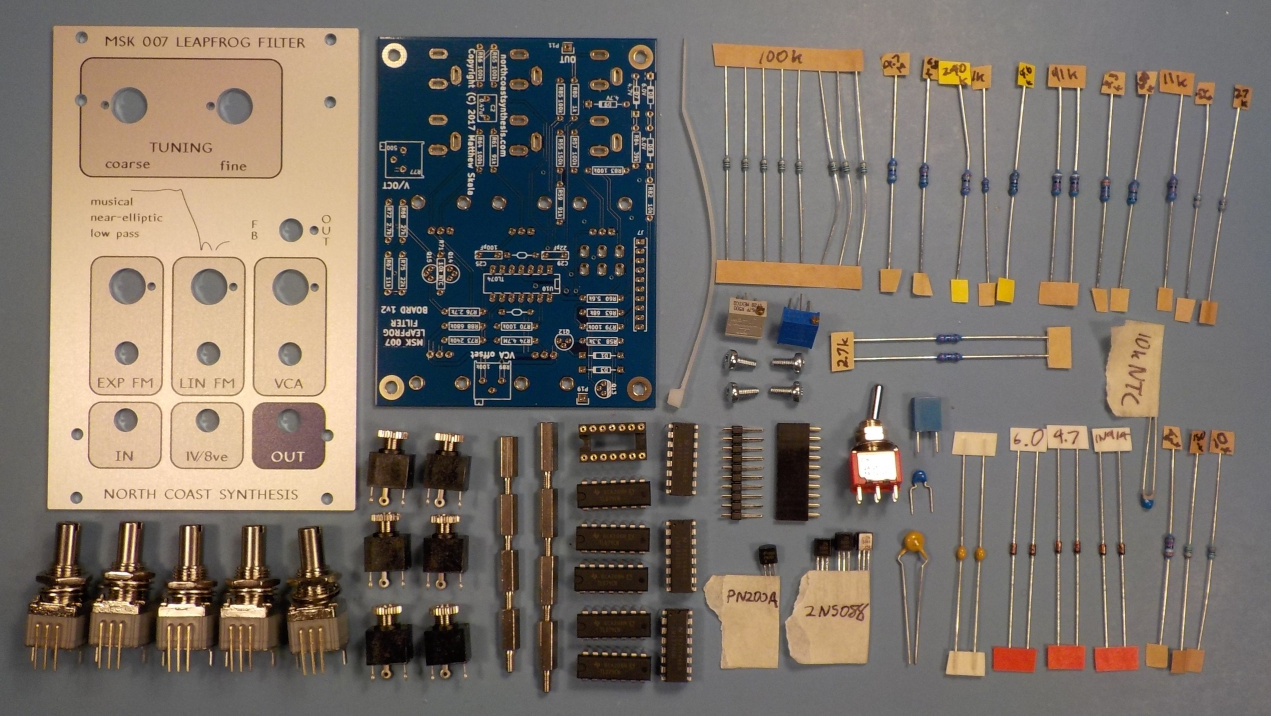
\includegraphics[width=\linewidth]{board1-parts.jpg}

There are two multiturn trimmers to be installed on this board.  Before
installing them, use an ohmmeter to adjust each one to 50\% of its range. 
Measure the resistance along the track, then measure the resistance from the
wiper to one end and adjust to make the wiper half the total track
resistance.  This need not be exact, but it will help with adjustment later,
by reducing issues with interaction among the different settings.  With all
trimmers pre-set to 50\%, the module should basically work even if it is not
at its best, whereas if many are installed at extreme values instead, then
you may have trouble getting it up and running enough to adjust it more
accurately.

\begin{table*}
{\centering
\fbox{This table is not a substitute for the text instructions.}
\vspace{\baselineskip}

\begin{tabular}{rp{1in}cp{3in}}
  \textbf{Qty} & \textbf{Ref} & \textbf{Value/Part No.} & \\ \hline
\input{bomdata-1.tex}
\end{tabular}\par}
\caption{Bill of Materials for Board~1.  Also needed:  knobs, a cable tie,
and module-to-rack mounting~hardware.}\label{tab:b1bom}
\end{table*}

\section{Some notes on knobs}

The first batch of knobs I ordered for North Coast products turned out to
have serious quality problems, specifically with the setscrews that hold the
knobs onto the potentiometer shafts.  Some of the screws had marginal
threads that would strip when the screw was tightened, and I ended up having
to do a bunch of extra testing and ship extra knobs to some customers to
replace any that might fail.  Later batches have also had issues, although
they're under better control now because the bad first batch served as a
warning to step up the testing procedures.  Starting with kits prepared in
August 2019, I switched to blue knobs with 100\%\ testing; in September
2020, I switched to a new manufacturer, and knobs that are a slightly darker
shade of blue.  Although all the knobs I ship in kits now have been tested
and passed at least twice, and should be fine to use, I am also shipping
spare setscrews in any kits with knobs from batches where a signficant
number of knobs failed testing.

Here are some things to be aware of as a kit builder.

\begin{itemize}
\item Some photos in these instructions were taken with the older grey
knobs, and some dealers may still have kits containing grey knobs in their
stock, but newer kits will have blue knobs.

\item Do not overtighten the setscrews when attaching the knobs!  The screw
should be tight enough to hold the knob onto the shaft, but there's no
advantage to making it tighter than that, and overtightening may risk
destroying the screw thread or damaging the drive slot.

\item If, despite my efforts to make sure no bad screws get sent to
customers, you still get a bad screw that cannot be tightened and no spare
for it, then please contact me.

\item If you want to source an exact replacement for the setscrew, it should
be an M3$\times$3mm flat-tip slotted setscrew, which is also sometimes
called a ``grub screw,'' made of RoHS-compliant brass (possibly by
exemption).  Stainless steel is fine too, and I may sometimes ship stainless
steel screws instead of brass if I can find a reliable source for them;
plain steel should not be used here for galvanic corrosion reasons. 
Hex-socket screws are fine if you have the driver for them, but I don't ship
those because I'm not sure all DIY builders do have the right driver.

\item Because it's a standard M3 thread, in a pinch it's possible to
substitute a plain M3 machine screw such as are commonly used with Eurorack
cases, although one of those would obviously look less nice.
\end{itemize}

\section{Fixed resistors}

Resistors are never polarized.  I like to install mine in a consistent
direction for cosmetic reasons, but this is electrically unnecessary.  In
this module, metal film 1\%\ resistors are recommended for all fixed-value
resistors.  These will usually have blue bodies and four colour bands
designating the value, plus a fifth band for the tolerance, brown in the
case of 1\%.  These are the resistors normally shipped in the
North Coast kits, but we may occasionally ship better-tolerance resistors (such
as 0.5\%) if we are able to source them at a good price. 
Accordingly, I mention only the four value band colours for this type of
resistor; if you are using resistors with other codes, you are responsible
for knowing them.  Note that colour codes on metal film 1\% resistors are
often ambiguous (reading from one end or the other end may give two
different values, both plausible) and some of the colours are hard to
distinguish anyway.  If in doubt, always measure with an ohmmeter before
soldering the resistor in place.

\pagebreak

Install the 1k$\Omega$ (brown-black-black-brown) resistor R80.  This
resistor limits the current that can flow on the module output, as well as
separating the output driver op amp and its stability capacitor from any
destabilizing capacitance that may be attached to the output (for instance,
from a long patch cable).  Do not confuse it with the other power-of-ten
resistor values (10k$\Omega$, 100k$\Omega$, and 1M$\Omega$).

\nopagebreak
\noindent\includegraphics[width=\linewidth]{{res-1.0k1}.jpg}

Install the two 2.7k$\Omega$ (red-violet-black-brown) resistors R72 and R76.
These resistors are used in the exponential converter, R72 as part of the
network that scales the control voltage and R76 to control voltage and
current at the output of the servo op amp.  Do not confuse them with the
27k$\Omega$ resistor, which has a similar colour code and is to be
mounted in a PCB footprint near that of R72.

\nopagebreak
\noindent\includegraphics[width=\linewidth]{{res-2.7k1}.jpg}

\pagebreak

Install the 3.3k$\Omega$ (orange-orange-black-brown) resistor R58.
This resistor is used in the linear voltage-to-current converter that
provides control current to the VCA section.

\nopagebreak
\noindent\includegraphics[width=\linewidth]{{res-3.3k1}.jpg}

Install the 5.6k$\Omega$ (green-blue-black-brown) resistor R60.
This resistor converts the exponential converter's output current back to a
voltage for broadcast to the five integrators.

\nopagebreak
\noindent\includegraphics[width=\linewidth]{{res-5.6k1}.jpg}

\pagebreak

Install the 10k$\Omega$ (brown-black-black-red) resistor R82.
This resistor sets the maximum attenuation of the VCA soft-clipping section. 
Do not confuse it with the other power-of-ten resistor values, nor the
11k$\Omega$ resistor.

\nopagebreak
\noindent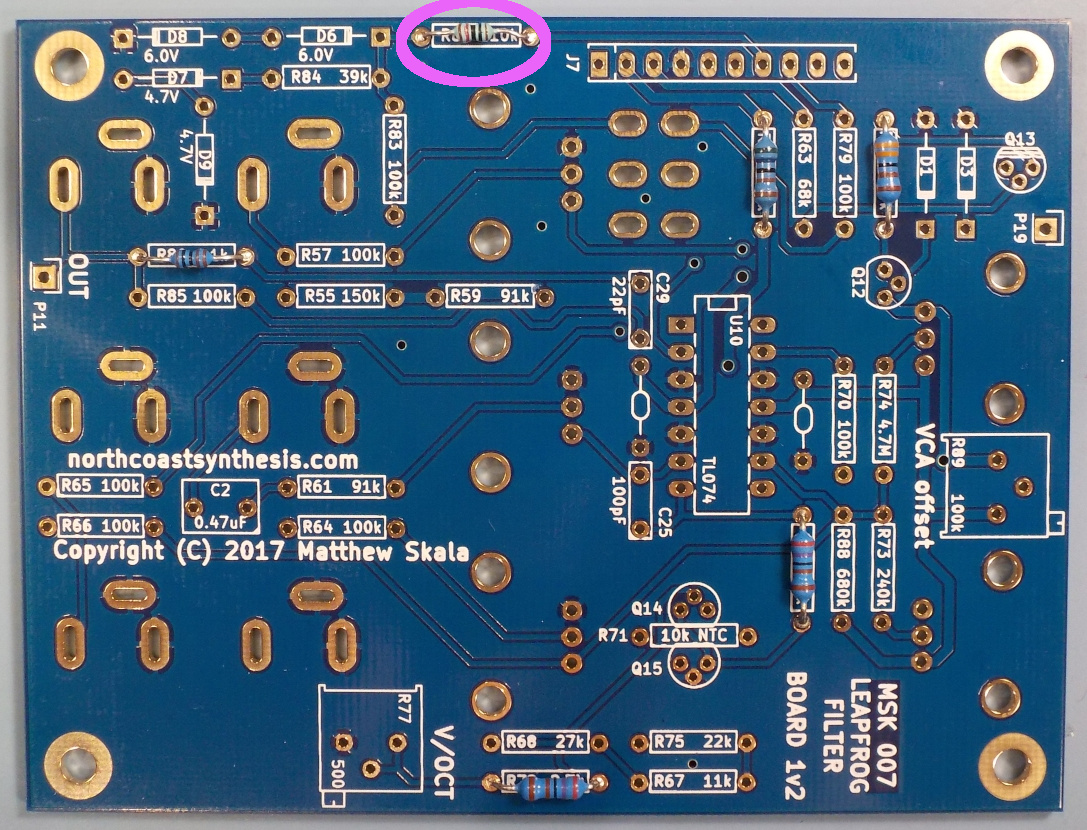
\includegraphics[width=\linewidth]{res-10k1.jpg}

Install the 11k$\Omega$ (brown-brown-black-red) resistor R67.
This resistor is part of the pitch control voltage scaling network.

\nopagebreak
\noindent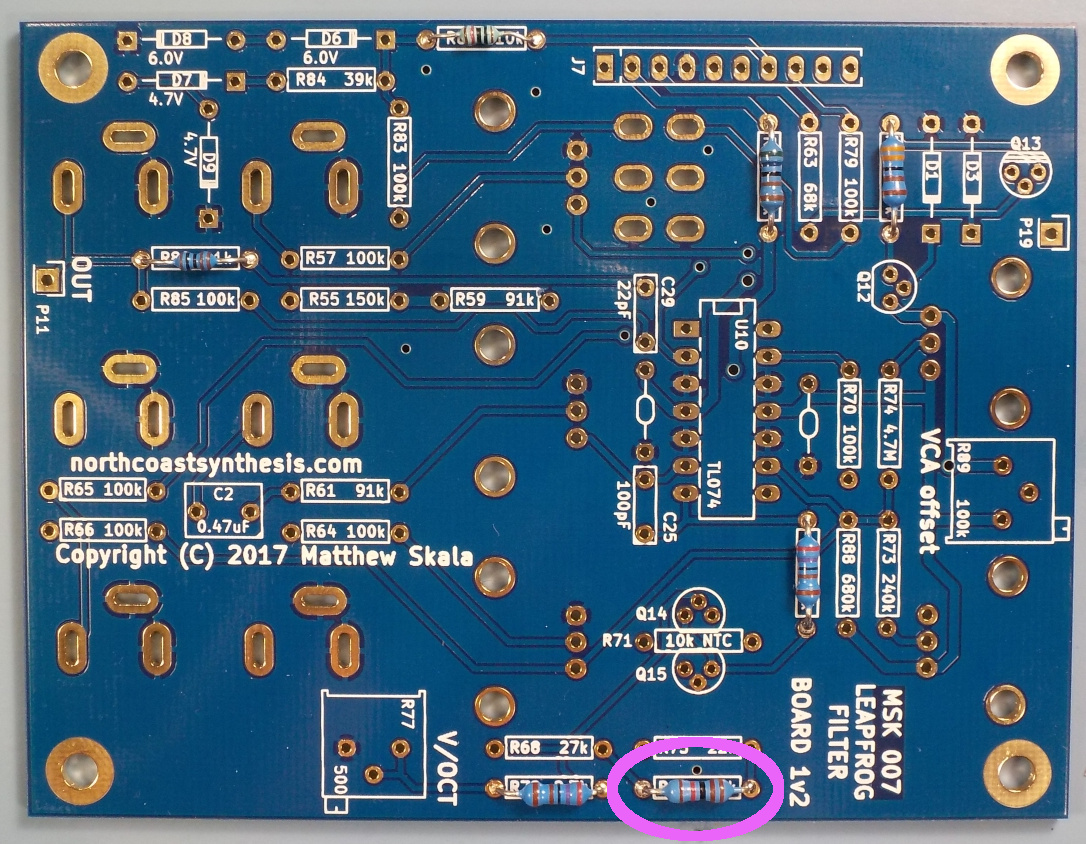
\includegraphics[width=\linewidth]{res-11k1.jpg}

\pagebreak

Install the 22k$\Omega$ (red-red-black-red) resistor R75.
This resistor sets the gain of the op amp in the control voltage scaling
network.

\nopagebreak
\noindent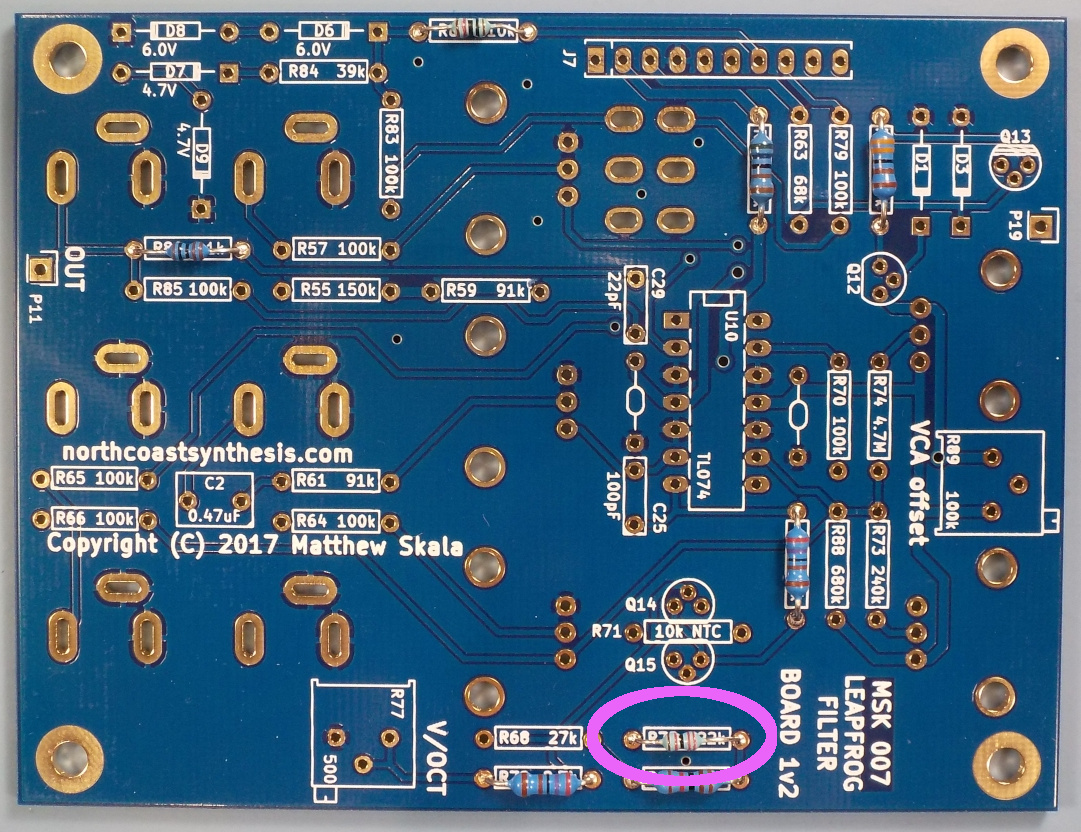
\includegraphics[width=\linewidth]{res-22k1.jpg}

Install the 27k$\Omega$ (red-violet-black-red) resistor R68.
This resistor is another part of the control voltage scaling network.

\nopagebreak
\noindent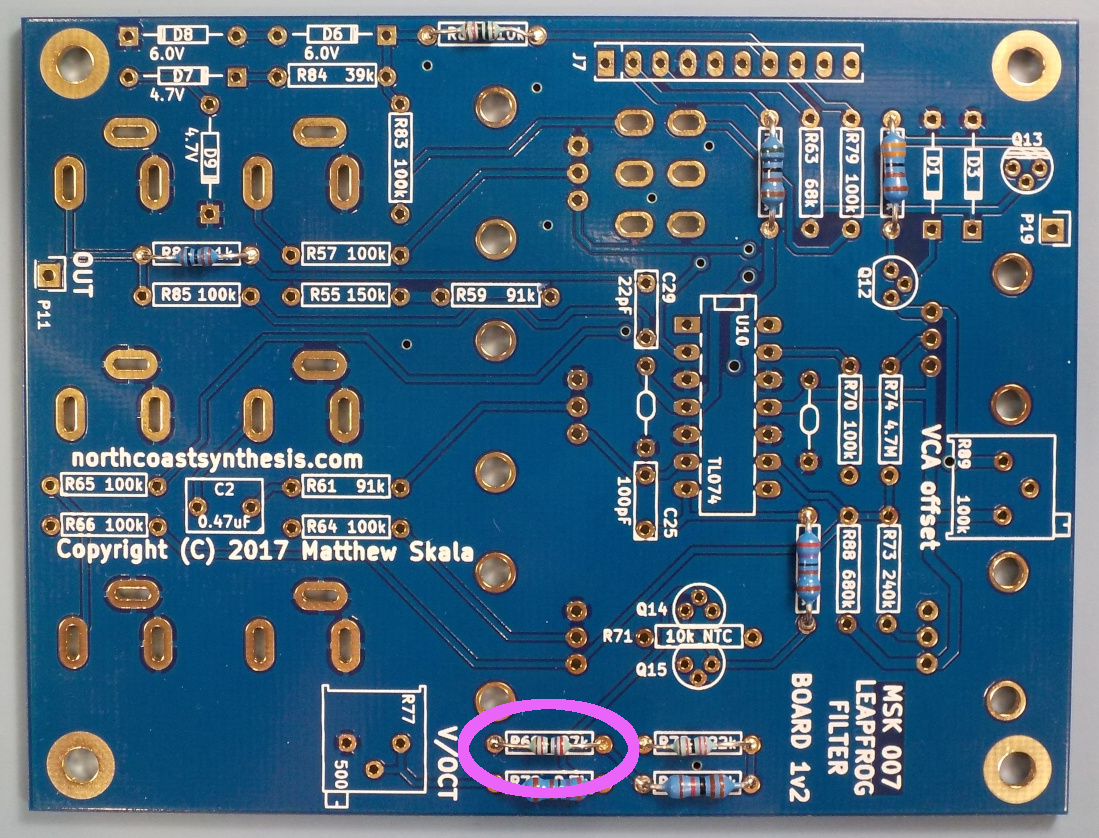
\includegraphics[width=\linewidth]{res-27k1.jpg}

\pagebreak

Install the 39k$\Omega$ (orange-white-black-red) resistor R84.
This resistor sets the mid-level attenuation of the VCA soft-clipping
circuit.

\nopagebreak
\noindent\includegraphics[width=\linewidth]{res-39k1.jpg}

Install the 68k$\Omega$ (blue-grey-black-red) resistor R63.
This resistor pulls down the base of the transistor Q13 to bring the VCA's
zero-gain point near 0V.  Do not confuse it with the 680k$\Omega$ resistor,
which has a similar colour code.

\nopagebreak
\noindent\includegraphics[width=\linewidth]{res-68k1.jpg}

\pagebreak

Install the two 91k$\Omega$ (white-brown-black-red) resistors R59 and R61. 
These two resistors set the reference current for the exponential converter,
and the maximum sensitivity of the linear FM input, respectively.

\nopagebreak
\noindent\includegraphics[width=\linewidth]{res-91k1.jpg}

Install the eight 100k$\Omega$ (brown-black-black-orange) resistors R57, R64
through R66, R70, R79, R83, and R85.
These resistors are used in multiple places throughout the input and output
circuits to either set input impedances to Eurorack standard, or set op amp
gain to negative unity by balancing against an input resistor.

\nopagebreak
\noindent\includegraphics[width=\linewidth]{res-100k1.jpg}

\pagebreak

Install the 150k$\Omega$ (brown-green-black-orange) resistor R55.
This resistor sets the DC normalization for the VCA control input.

\nopagebreak
\noindent\includegraphics[width=\linewidth]{res-150k1.jpg}

Install the 240k$\Omega$ (red-yellow-black-orange) resistor R73.
This resistor sets the range of the coarse tuning knob to about ten
octaves.

\nopagebreak
\noindent\includegraphics[width=\linewidth]{res-240k1.jpg}

\pagebreak

Install the 680k$\Omega$ (blue-grey-black-orange) resistor R88.
This resistor sets the overall offset of the tuning knobs, for a
non-guaranteed design target of approximately 10Hz to 10kHz cutoff frequency
with zero pitch control voltage.

\nopagebreak
\noindent\includegraphics[width=\linewidth]{res-680k1.jpg}

Install the 4.7M$\Omega$ (yellow-violet-black-yellow) resistor R74.
This resistor sets the range of the fine tuning knob to about half an
octave.

\nopagebreak
\noindent\includegraphics[width=\linewidth]{{res-4.7m1}.jpg}

\section{Diodes}

There are six diodes to be mounted on Board~1:  two each of 1N4148 or 1N914
switching diodes; 1N5230B 4.7V Zener diodes; and 1N5223B 6.0V Zener diodes. 
They all look like pretty much identical orange-pink glass beads, and it is
important not to confuse them.  Their bodies will be marked with type
numbers in very small print, and they should be labelled in a kit, but if
you are in any doubt, test them for breakdown voltage.

\pagebreak

To do a breakdown voltage test:  use clip leads or a breadboard to connect
the diode under test in series with a small resistor (anything from
1k$\Omega$ to 10k$\Omega$) reverse biased across a 12V power supply.  That
is, the power supply positive connects to one end of the resistor, the other
end of the resistor connects to the cathode (striped end) of the diode, and
the anode (other end) of the diode connects to the power supply negative. 
Then measure the voltage across the diode.  It should be close to the
specified Zener voltage of 4.7V or 6.0V if you are testing a Zener diode,
and equal to the power supply voltage if you are testing one of the
switching diodes.  From that it should be possible to determine which diodes
are which.  If the measured value is less than 1V, then you most likely have
the diode backwards and are measuring its \emph{forward} voltage, which will
be about the same for all three of these diode types and is not a useful way
to distinguish them.

All these diodes are polarized components and it is important to install
them right way round.  Each diode has a black stripe at one end; that end is
the \emph{cathode}.  The silkscreen markings on the board have a
corresponding stripe and the diodes should be installed with their stripes
matching the markings on the board.  The solder pads for the cathodes are
also square instead of round.

Install the two 1N4148 or 1N914 switching diodes D1 and D3.  These are used
to control the minimum base voltages for the transistors in the VCA section.

\nopagebreak
\noindent\includegraphics[width=\linewidth]{1n4148.jpg}

\pagebreak

Install the two 1N5230B Zener diodes D7 and D9.  Their breakdown voltage of
4.7V is marked on the silkscreen as an additional guide to where they go. 
These set the lower voltage level for the soft-clipping circuit.

\nopagebreak
\noindent\includegraphics[width=\linewidth]{{zener-4.7v1}.jpg}

Install the two 1N5233B Zener diodes D6 and D8.  Their breakdown voltage of
6.0V is marked on the silkscreen as an additional guide to where they go. 
These set the higher voltage level for the soft-clipping circuit.

\nopagebreak
\noindent\includegraphics[width=\linewidth]{{zener-6.0v1}.jpg}

\section{DIP sockets}

Install the 14-pin DIP socket for the TL074 quad op amp chip U10.  The
amplifiers in this chip are used in the exponential converter and as buffers
between the filter core and the outside world.  See
page~\pageref{pag:dip-sockets} for notes regarding orientation of the
socket, procedure for soldering it flat to the board, and so on.

\noindent\includegraphics[width=\linewidth]{dip14-1.jpg}

\section{Trimmer potentiometers}

If you have not already set the trimmers to 50\%\ of their full scale value
as described under ``Preliminaries'' above, then do it now.

Trimmers are not exactly polarized, but the three legs of each trimmer serve
different functions and need to be connected to the right holes.  The
physical arrangement of the legs and corresponding holes should make it
impossible to install the trimmers wrong way round.

Install the 500$\Omega$ trimmer R77.  This trimmer sets the scale factor for
the V/octave pitch CV, an adjustment often called ``tracking.''

\nopagebreak
\noindent\includegraphics[width=\linewidth]{pot-500w1.jpg}

\pagebreak

Install the 100k$\Omega$ trimmer R89.  This trimmer adjusts the DC offset in
the VCA section.

\nopagebreak
\noindent\includegraphics[width=\linewidth]{pot-100k1.jpg}

\section{Capacitors}

Small-valued ceramic capacitors are usually labelled with numbers in a
pattern similar to the resistor colour code:  two digits for the main value,
followed by a third digit that says how many zeroes to append to get the
value in picofarads.  Thus the 22pF capacitor may be labelled ``220'' and
the 100pF capacitor ``101.''  Other markings on the capacitor body may
indicate tolerance, voltage rating, dielectric type, and so on.  The
0.1$\mu$F decoupling capacitors will probably have very abbreviated markings,
but if they are labelled on the three-digit system the code would be ``104''
for 0.1$\mu$F $=$ 100000pF (10 followed by 4 additional zeroes);
and the box-type 0.47$\mu$F film capacitor will likely be marked with its
value in microfarads using $\mu$ instead of the decimal point, thus
``$\mu$47.''  None of the capacitors to be installed on this board are
polarized.

\pagebreak

Install the 22pF ceramic capacitor C29.  This capacitor prevents
high-frequency oscillation of the output driver op amp.

\nopagebreak
\noindent\includegraphics[width=\linewidth]{cap-22p1.jpg}

Install the 100pF ceramic capacitor C25.  This capacitor prevents
high-frequency oscillation of the exponential converter servo op amp.

\nopagebreak
\noindent\includegraphics[width=\linewidth]{cap-100p1.jpg}

\pagebreak

Install the two 0.1$\mu$F decoupling capacitors.  As described on
page~\pageref{pag:decoup-symbol}, they are shown on the board silkscreen by
a special symbol without values or reference designators.  They filter the
power supplies for the op amp chip.

\nopagebreak
\noindent\includegraphics[width=\linewidth]{{cap-0.1u1}.jpg}

Install the 0.47$\mu$F film capacitor C2.  This capacitor provides AC
coupling for the linear FM input.

\nopagebreak
\noindent\includegraphics[width=\linewidth]{{cap-0.47u1}.jpg}

\pagebreak

\section{TO-92 semiconductors}

See page~\pageref{pag:to-92} for general instructions regarding TO-92
semiconductors and the board symbols used for them.

Install the PNP transistor Q13, type SS8550D or PN200A.  This transistor
acts as a current source for controlling the VCA section.

\nopagebreak
\noindent\includegraphics[width=\linewidth]{pn200a-1.jpg}

Install the 2N5088 NPN amplifier transistor Q12.  This transistor acts as an
emitter follower to translate the input control voltage to a current for
Q13.  There are two more 2N5088 transistors to be installed in the next
section.

\nopagebreak
\noindent\includegraphics[width=\linewidth]{2n5088-1.jpg}

\section{Exponential converter cluster}

In order to reduce the temperature dependence of the exponential converter
as far as possible, is is important that the two transistors Q14 and Q15,
and the thermistor (temperature-sensitive resistor) R71, should all be kept
at the same temperature.  This is accomplished by mounting them all in
contact with each other and tightening a nylon cable tie around them to keep
them pressed together.  Constructing this cluster of components is a little
tricky and annoying; follow the directions carefully.

Bend the thermistor legs as shown:  one leg straight down, the other down
about 3mm, then to the side, then down again, to fit the R71 footprint. 
Place the thermistor in its footprint, but do not solder it yet.

\nopagebreak
\noindent\includegraphics[width=\linewidth]{ntc-bend.jpg}

Insert the two 2N5088 transistors Q14 and Q15 in the board, face to face as
shown.  Do not solder them yet.

\nopagebreak
\noindent\includegraphics[width=\linewidth]{expo-untied.jpg}

\pagebreak

Put a nylon cable tie around the three components and tighten it far enough
to hold them loosely together.  Concentrate in particular on having the two
transistors meet as cleanly face to face as possible.  Do not overtighten
the cable tie or cut it off yet.  This is probably the hardest step, and
North Coast kits include a spare cable tie for use in case you ruin one.  Be
aware that the components should not stick out any further above the board
than is normal for other TO-92 components; if you seat the transistors too
high up, at the full length of their legs, you may exceed the 11mm of
clearance between this board and Board~2 above it.

Solder the components.  Then tighten the cable tie the rest of the way and
cut off the excess.

\nopagebreak
\noindent\includegraphics[width=\linewidth]{expo-tied.jpg}

\pagebreak

\section{Board to board connectors}

Screw one 13mm and one 11mm standoff into each of the four mounting holes in
Board~1, as shown.  The shorter (11mm) standoff should be on the top, the
same side as the components already installed, with the male-threaded ends
sticking up.  These standoffs will separate Board~1 from Board~2 in the
final module.  The longer (13mm) standoffs should be on the bottom, with
their male ends passing through the board to mate with the 11mm standoffs.

\nopagebreak
\noindent\includegraphics[width=\linewidth]{board12-stack-1.jpg}

Mate the 10$\times$1 header connectors J7 and P26 and place them (do not
solder yet) in the J7 footprint on Board~1 with the legs of the female
connector J7 going through the board.

\nopagebreak
\noindent\includegraphics[width=\linewidth]{board12-stack-2.jpg}

\pagebreak

Place your completed Board~2 from the previous chapter on top of the
assembly, component side up with the legs of P26 going through the P26
footprint, and fasten it with the remaining four 11mm standoffs.

\nopagebreak
\noindent\includegraphics[width=\linewidth]{board12-stack-3.jpg}

Solder J7 and P26 in place on the two boards.  Then remove Board~2 and the
four standoffs holding it in place, but keep the standoffs that go through
the holes in Board~1.

\section{Panel components}

Flip Board~1 over; you will now be installing the components that go between
it and the panel.  The exact details of how the pieces fit together are
important and may not be obvious; see the exploded assembly diagram on
page~\pageref{fig:exploded}, which may clarify things.

The toggle switch SW3 is for switching the VCA section between providing
feedback and controlling the output.  It has a body just a little shorter
than will fit well into the 13mm space between Board~1 and the panel.  This
space is forced to be 13mm to accommodate the potentiometer bodies.  The
switch comes with two nuts and only needs one for fastening on the front of
the panel.  We use the second one as a spacer behind the panel to hold the
switch body far enough back that its legs will go through the holes in the
board.  Remove and save the hardware from the switch bushing, then screw on
one of the nuts all the way down to the bottom of the bushing.

The switch's electrical connections are symmetrical, but it has a slot or
keyway in its bushing, used to hold the special anti-rotation washer in
place.  This keyway must face toward the outer edge of the board in order
for the anti-rotation washer to be able to connect \pagebreak the switch
properly with a matching small hole in the panel.  Place (do not solder yet)
the switch in its footprint on Board~1, with the keyway facing outward.

\nopagebreak
\noindent\includegraphics[width=\linewidth]{switch-keyway.jpg}

Place (do not solder yet) the five panel control potentiometers R56, R62,
R69, R78, and R81 in their footprints on the board.  These provide manual
control of the module's functions.  Place (do not solder
yet) the six phone jack sockets J1 through J6 in their footprints.  These
are for patching signals to and from other modules.  All these components
should only be able to fit into the board in one way.

\nopagebreak
\noindent\includegraphics[width=\linewidth]{panel-components.jpg}

Line up the panel on top of the asembly and fasten it in place by driving
the four machine screws through their corresponding holes into the 13mm
standoffs.  Double check that the keyway on the switch bushing is facing the
small hole near the switch which will accept the alignment tab from the
anti-rotation washer.

\noindent\includegraphics[width=\linewidth]{panel-screws.jpg}

Install all the hardware for the panel components.  In the case of the
switch, the sequence is first (nearest the panel) the anti-rotation washer,
with one of its tabs fitting into the keyway on the bushing and the other
sticking into the small panel hole provided for this purpose; then the
toothed lock-washer (sharper side of the teeth facing up to engage with the
nut, if there's a noticeable difference between the two sides); and finally
the nut.  In the case of the potentiometers, the sequence is first (nearest
the panel) the conical spring washer, high side in the middle and low side
around the outside; then the toothed lock-washer; then the nut.

In the case of the jack sockets, the knurled nuts provided for these will
have screwdriver slots on one side, and those should face the outside with
the smoother side facing the panel.  You may need to tilt the assembly and
jiggle it a bit to get the jack sockets to fall into the right alignment
with their bushings poking through the panel.  On the other side, when
correctly installed their solder legs (and those of the switch) will just
barely pass through the circuit board.

Do not overtighten any of this hardware, and be careful, if you are
using wrenches or pliers, to avoid scratching the panel.  Wrapping the tool
jaws with tape may help.

\nopagebreak
\noindent\includegraphics[width=\linewidth]{panel-hardware.jpg}

Solder the panel components.  It can be tricky to do the joints where a
component leg just barely passes through the board, but if you take it slow
and make sure that the PCB hole is filled with solder and the whole joint is
liquid before you remove the heat, then you can be reasonably sure that you
have wetted the leg and made a good electrical connection.  It may help to
use a larger-than-usual soldering iron tip if you have one.

\pagebreak

\section{Final assembly}

Attach the knobs to the potentiometers.  Twist each shaft to its limits in
each direction to ascertain how the slot in the shaft corresponds to where
you want the knob pointer, then slide the knob onto the shaft in the correct
orientation and tighten the setscrew with a small flat screwdriver.  See the
comments at the start of this chapter about knobs, and be sure not to
overtighten the setscrews when attaching them.

Insert a TL047 chip in the U10 socket on Board~1.  Be careful to insert it
right way round: the end with Pin 1 will be marked by an indentation at one
corner or a notch in the end and this end of the chip should be inserted to
match the notch in the socket and on the board silkscreen and the
rectangular Pin 1 solder pad.

Also be careful that all the legs of the chip go into the corresponding
holes in the socket.  These chips, when brand new, usually have their legs
splayed outward a little bit (a measure intended to help them fit snugly
into circuit boards when used without a socket) and you must gently bend the
legs inward in order to fit them in the sockets.  If you apply pressure to a
chip prematurely, without all the legs properly fitting into the holes, it
is easy to have the legs fold up or even break off.

It should not be necessary to remove the panel from Board~1 again.  Attach
Board~2, carefully fitting its header plug into the header socket on Board~1
and the male ends of the standoffs through the corresponding holes in Board~2. 
Screw on the remaining 11mm standoffs to hold it in place.

Insert the remaining four TL074 chips and the three LM13700 chips in their
corresponding sockets.  See the notes above on inserting DIP chips in
general, and pay special attention to the directional markings on the board
silkscreen and the notches in the sockets to make sure you have them
installed in the right directions.

If you have not yet done the ``pre-adjustment'' described in the next
chapter, do it now, before assembling Board~3 with the rest of the module. 
But assuming that is complete, add Board~3 to the assembly, fitting its
three male header connectors into the header sockets on Board~2, and screw
on the four hex nuts to hold it in place.  Be careful with your nutdriver,
pliers, or other tools not to damage other components near the nuts on
Board~3.  If using a nutdriver, socket wrench, or similar, be careful not to
overtighten the nuts:  some tools make it easy to apply more torque than the
threads can sustain.

\pagebreak

There is a rectangular white area on Board~3
reserved for adding a serial number, signature, quality control marking, or
similar.  Use a fine-tipped permanent marker to write whatever you want
there.

Your module is complete.

\nopagebreak
\noindent\includegraphics[width=\linewidth]{finished-module.jpg}

% $Id: preadjustment.tex 5860 2018-01-23 22:23:18Z mskala $

%
% MSK 007 pre-adjustment procedure
% Copyright (C) 2017  Matthew Skala
%
% This program is free software: you can redistribute it and/or modify
% it under the terms of the GNU General Public License as published by
% the Free Software Foundation, version 3.
%
% This program is distributed in the hope that it will be useful,
% but WITHOUT ANY WARRANTY; without even the implied warranty of
% MERCHANTABILITY or FITNESS FOR A PARTICULAR PURPOSE.  See the
% GNU General Public License for more details.
%
% You should have received a copy of the GNU General Public License
% along with this program.  If not, see <http://www.gnu.org/licenses/>.
%
% Matthew Skala
% https://northcoastsynthesis.com/
% mskala@northcoastsynthesis.com
%

\chapter{Pre-adjustment}\label{ch:preadj}

To complete the preadjustment process you will need an
ohmmeter; a tool (probably a small slotted screwdriver) to adjust the
trimmers; and your completed Board~3.  A Eurorack power supply and voltmeter
are optional.

Note this procedure is to be done on
Board~3 \emph{disconnected} from any other boards; the measurements will not
be correct if it is attached to the other boards. 
Figure~\ref{fig:board3-silk} shows the silkscreen art for Board~3, which may
help to locate the trimmers and test points.  Version~3 of the art is
shown; if you have one of the earlier Version~2 boards, all the trimmers and
test points are in the same places, but there are minor differences in some
of the label positions.

Throughout these instructions, calculated target values for the measurements
are given to more precision than it is usually practical to measure or
adjust.  Just round them off to the appropriate level for what your test
equipment can do.

\begin{figure*}
\centering\includegraphics[angle=-90,scale=1.5]{board3-silk.eps}
\caption{Board~3 silkscreen art}\label{fig:board3-silk}
\end{figure*}

\section{Short-circuit test}

This check will be done again on the entire module during the regular
adjustment phase, but it's worth doing it right at the start on Board~3
alone to help narrow down any problems you might discover.

The two pins on the Eurorack power connector nearest the edge of Board~3
(at the bottom when the module is mounted upright in a case) are for the
$-$12V connection.  That is the end where the red stripe on the cable would
normally connect.  The two pins at the other end of the connector (furthest
from the edge of the board) are for $+$12V power.  All six pins in the
middle are for 0V (ground).

\noindent\includegraphics[width=\linewidth]{power-pinout.jpg}

Check for shorts between the three power connections, testing each pair in
both directions (six tests in all).  Ideally, you should use an ohmmeter's
``diode test'' range for this, and it should read infinite in the reverse
direction (positive lead to $-$12V and negative lead to each of the other
two, as well as positive lead to ground and negative to $+$12V) and greater
than 1V in the forward direction (reverse those three tests).  If any of
these six measurements is less than 100$\Omega$ or 1V, then something is
wrong with the build and you should troubleshoot it before applying power.

\section{Integrator time constants}

Each of the five integrator stages has a time constant controlled primarily
by a trimmer.  At this point we set these roughly by setting the resistances
to values that would be correct if all other components in the circuit had
their design values; in the later, more precise adjustment step, the values
may be modified to compensate for variations in those other components.

Measure the resistance between P1 ``+9V TC CMN'' (that is, ``time constant
common''; the test point is connected to what will be the internal +9V
supply when the module is fully assembled) and P2 ``TC~A'' and adjust R7 to
bring this resistance to 7.9856k$\Omega$.

Measure the resistance between P1 ``+9V TC CMN'' and P3 ``TC~B'' and adjust
R8 to bring this resistance to 6.8802k$\Omega$.

Measure the resistance between P1 ``+9V TC CMN'' and P4 ``TC~C'' and adjust
R9 to bring this resistance to 4.4816k$\Omega$.

Measure the resistance between P1 ``+9V TC CMN'' and P5 ``TC~D'' and adjust
R26 to bring this resistance to 8.1997k$\Omega$.

Measure the resistance between P1 ``+9V TC CMN'' and P6 ``TC~E'' and adjust
R27 to bring this resistance to 7.4310k$\Omega$.

\section{Output mix}

The output of the filter is a carefully chosen fixed mixture of the output
signals from the five integrator stages.  There is an interaction between
the R43 and R34 adjustments, hence their repetition in these instructions;
the stated sequence should minimize any problems caused by interaction.

Measure the resistance between P22 ``mix~$-$'' and P16 ``mix~E'' and adjust
R43 to bring this resistance to 4.2802k$\Omega$.

Measure the resistance between P23 ``mix~$+$'' and P13 ``mix~D'' and adjust
R38 to bring this resistance to 25.144k$\Omega$.

Measure the resistance between P22 ``mix~$-$'' and P10 ``mix~C'' and adjust
R34 to bring this resistance to 19.3130k$\Omega$.

Measure the resistance between P23 ``mix~$+$'' and P9 ``mix~B'' and adjust
R32 to bring this resistance to 890.04k$\Omega$.

Measure the resistance between P22 ``mix~$-$'' and P8 ``mix~A'' and adjust
R30 to bring this resistance to 961.04k$\Omega$.

Measure the resistance between P22 ``mix~$-$'' and P16 ``mix~E'' a second
time; it should be near 4.2802k$\Omega$.  If necessary, adjust
R43 to make it exactly 4.2802k$\Omega$.

Measure the resistance between P22 ``mix~$-$'' and P10 ``mix~C'' a second
time; it should be near 19.3130k$\Omega$.  If necessary, adjust
R34 to make it exactly 19.3130k$\Omega$.

Note the footprint labelled R28, corresponding to the test point P7
``mix~IN,'' is meant for reusing this board design with other filter curves;
in the standard lowpass configuration there is no trimmer there and no
adjustment needed.

\section{DC offset trim}

The DC offset trimmer R50 should be set to its midpoint for now; it
will be adjusted up or down to compensate offset in the OTA chips later.
If you followed the build instructions carefully, then you will have set it
to its midpoint before installing it and no further adjustment is needed at
this point.

Otherwise, connect the board to a Eurorack power supply, and confirm that
+12V appears on test point P12 and -12V on P15, relative to any convenient
grounded point on the board (such as the mounting hole nearby) and to within
the voltage tolerance of your power supply.  Measure the voltage on P14
labelled ``DC'' and adjust R50 to bring the measured voltage to zero.

Alternate procedure:  instead of connecting the board to a power supply, you
can measure the resistances among P14, P12 (labelled $+$12V), and P15
(labelled $-$12V).  The wiper of the 100k$\Omega$ trimmer is connected to
P14 and the two ends of the track are connected to P12 and P15, so with no
power applied to the board, you can adjust for equal resistances (of
50k$\Omega$ subject to tolerance) between P12 and P14 and between P14 and
P15.

% $Id: adjustment.tex 8331 2020-11-19 05:17:40Z mskala $

%
% MSK 011 testing and adjustment instructions
% Copyright (C) 2018  Matthew Skala
%
% This program is free software: you can redistribute it and/or modify
% it under the terms of the GNU General Public License as published by
% the Free Software Foundation, version 3.
%
% This program is distributed in the hope that it will be useful,
% but WITHOUT ANY WARRANTY; without even the implied warranty of
% MERCHANTABILITY or FITNESS FOR A PARTICULAR PURPOSE.  See the
% GNU General Public License for more details.
%
% You should have received a copy of the GNU General Public License
% along with this program.  If not, see <http://www.gnu.org/licenses/>.
%
% Matthew Skala
% https://northcoastsynthesis.com/
% mskala@northcoastsynthesis.com
%
\chapter{Adjustment and testing}

The MSK~011 is designed to work with very little adjustment.  As a result of
its minimalist transistor-based design, there is unavoidably some
temperature-sensitive offset in the DC-coupled output.  A trimmer is
provided to help null this out, but because of the temperature sensitivity
the offset will probably never remain at zero in practical use.  For audio
applications it is preferable to use the AC-coupled output.

This adjustment procedure requires the finished module, a smallish cross-tip
screwdriver, a suitable power supply, and a multimeter.

\section{Short-circuit test}

With no power applied to the module, check for short circuits between the
three power connections on the Eurorack power connector.  The two
pins at the bottom, marked with an arrow on the circuit board, are for -12V. 
The two at the other end are for +12V; and the remaining six pins in the
middle are all ground pins.  Check between each pairing of these three
voltages, in both directions (six tests in all).  Ideally, you should use a
multimeter's ``diode test'' range for this; if yours has no such range, use
a low resistance-measuring setting. It should read infinite in the reverse
direction (positive lead to $-$12V and negative lead to each of the other
two, as well as positive lead to ground and negative to $+$12V) and greater
than 1V or 1k$\Omega$ in the forward direction (reverse those three
tests).  If any of these six measurements is less than 1k$\Omega$ or 1V,
then something is wrong with the build, most likely a blob of solder
shorting between two connections, and you should troubleshoot that before
applying power.

\emph{Optional}:  Although we test all cables before we sell them, bad
cables have been known to exist, so it might be worth plugging the Eurorack
power cable into the module and repeating these continuity tests across the
cable's corresponding contacts (using bits of narrow-guage wire to get into
the contacts on the cable if necessary, or probing the pins of the power
connector on the back side of the circuit board) to make sure there are no
shorts in the cable crimping.  Doing this test \emph{with the cable
connected to the module} makes it easier to avoid mistakes, because the
module itself will short together all wires that carry equal potential,
making it easier to be sure of testing the relevant adjacent-wire pairs in
the cable.

Plug the module into a Eurorack power supply and make sure
neither it nor the power supply emits smoke, overheats, makes any unusual
noises, or smells bad.  If any of those things happen, turn off the power
immediately, and troubleshoot the problem before proceeding.

\emph{Optional}: Plug the module into a Eurorack power supply
\emph{backwards}, see that nothing bad happens, and congratulate yourself on
having assembled the reverse-connection protective circuit properly. 
Reconnect it right way round before proceeding to the next step.

\section{Output offset adjustment}

Turn all knobs fully counterclockwise.  Apply power to the module with
nothing plugged into the input, and measure the DC voltage of the DC-coupled
output.  Adjust R7 at the top of the board, labelled ``offset null,'' to
bring the output as close to 0V as is reasonably possible.  It is unlikely
that you will be able to get it to stay at exactly zero.

% $Id: patches.tex 5703 2017-10-31 03:07:37Z mskala $

%
% MSK 007 patch ideas
% Copyright (C) 2017  Matthew Skala
%
% This program is free software: you can redistribute it and/or modify
% it under the terms of the GNU General Public License as published by
% the Free Software Foundation, version 3.
%
% This program is distributed in the hope that it will be useful,
% but WITHOUT ANY WARRANTY; without even the implied warranty of
% MERCHANTABILITY or FITNESS FOR A PARTICULAR PURPOSE.  See the
% GNU General Public License for more details.
%
% You should have received a copy of the GNU General Public License
% along with this program.  If not, see <http://www.gnu.org/licenses/>.
%
% Matthew Skala
% https://northcoastsynthesis.com/
% mskala@northcoastsynthesis.com
%

\chapter{Patch ideas}

Here's a basic subtractive synthesis patch:  pitch CV from the MIDI
interface connects to the V/octave inputs on a sawtooth oscillator and the
MSK~007, while the gate CV drives and ADSR envelope which controls the
built-in VCA on the MSK~007 (VCA mode switch set to ``output'').

\nopagebreak\noindent
{\hspace*{\fill}\includegraphics[scale=0.6]{patch1.png}\hspace*{\fill}\par} 

In a more elaborate subtractive synthesis patch, two ADSR envelopes drive
the amplitude and filter cutoff separately, with an external VCA which frees
the MSK~007's built-in VCA to provide feedback.

\nopagebreak\noindent
{\hspace*{\fill}\includegraphics[scale=0.45]{patch2.png}\hspace*{\fill}\par} 

Deluxe subtractive synthesis patch demonstrating the use of the MSK~007 with
other North Coast Synthesis modules: the pitch CV goes through an MSK~008
Octave Switch (normalled to both channels) to provide separate manual octave
switching up and down for the VCO and the filter.  A sine wave from the
MSK~010 controls linear frequency modulation of the filter cutoff for a
unique effect.

\nopagebreak\noindent
{\hspace*{\fill}\includegraphics[scale=0.45]{patch3.png}\hspace*{\fill}\par} 

\pagebreak

The MSK~007 can be a minimal synth voice all by itself, using the
gate input to control the VCA in feedback mode to switch oscillation on and
off.  A MIDI interface is shown, but any CV-gate controller would work.

\nopagebreak\noindent
{\hspace*{\fill}\includegraphics[scale=0.6]{patch4.png}\hspace*{\fill}\par} 

An envelope generator set up to create a spike (fast attack and decay,
zero sustain level) can ``ping'' the filter when fed into the audio input. 
Set the VCA to feedback mode and adjust the level to the point where it
almost, but not quite, sustains oscillation.

\nopagebreak\noindent
{\hspace*{\fill}\includegraphics[scale=0.6]{patch5.png}\hspace*{\fill}\par}

Pinging with a noise burst instead of just a voltage spike produces a
different sound with some extra grit in the attack.

\nopagebreak\noindent
{\hspace*{\fill}\includegraphics[scale=0.6]{patch6.png}\hspace*{\fill}\par} 

\pagebreak

The MSK~007 can take inputs all the way down to DC, so
with the cutoff frequency very low (at or near its minimum) it can process
control voltages as
an unusual kind of slew rate limiter, with a bit of bounce or overshoot on
rapidly-changing inputs (especially in feedback mode).  The gain through the
filter is not easy to adjust to precisely unity, so you might not want to
use this for critical melodic material; but with a square wave LFO input, as
shown, it puts an interesting twist on the control waveform for generating
a drone texture.

\nopagebreak\noindent
{\hspace*{\fill}\includegraphics[scale=0.6]{patch7.png}\hspace*{\fill}\par} 

Doepfer's A-188-1 bucket brigade module does not include an output filter,
so at low clock rates the clock will be audible unless you filter it out
externally.  The MSK~007 is especially well-suited for that because of its
low cutoff.  With the MSK~007 tuned to cut off at the Nyquist frequency
(half the BBD's clock frequency), it will cleanly eliminate both clock and
alias signals.

\nopagebreak\noindent
{\hspace*{\fill}\includegraphics[scale=0.6]{patch8.png}\hspace*{\fill}\par} 

Spectral inversion is another use for a sharp low-pass filter.  Tune the
sine wave VCO (here used as a \emph{local oscillator}) to generate a carrier
a little above the highest frequency in the input.  Ring-modulate
(four-quadrant multiply) the input with the carrier.  That produces two
frequency bands: upper sideband consisting of the input shifted up by the
carrier frequency, and lower sideband consisting of all the input
frequencies subtracted from the carrier frequency.  The MSK~007
removes the upper sideband and any carrier feedthrough.

Spectral inversion is an interesting effect in itself, but you can also use
two copies of this patch (two MSK~007 modules, two oscillators,
and two channels of four-quadrant multiplication) with slightly
different carrier frequencies, to serve as a frequency shifter.

\nopagebreak\noindent
{\hspace*{\fill}\includegraphics[scale=0.6]{patch9.png}\hspace*{\fill}\par} 

% $Id: circuit.tex 9313 2021-08-07 16:45:06Z mskala $

%
% MSK 007 circuit explanation
% Copyright (C) 2017, 2021  Matthew Skala
%
% This program is free software: you can redistribute it and/or modify
% it under the terms of the GNU General Public License as published by
% the Free Software Foundation, version 3.
%
% This program is distributed in the hope that it will be useful,
% but WITHOUT ANY WARRANTY; without even the implied warranty of
% MERCHANTABILITY or FITNESS FOR A PARTICULAR PURPOSE.  See the
% GNU General Public License for more details.
%
% You should have received a copy of the GNU General Public License
% along with this program.  If not, see <http://www.gnu.org/licenses/>.
%
% Matthew Skala
% https://northcoastsynthesis.com/
% mskala@northcoastsynthesis.com
%

\chapter{Circuit explanation}

The MSK~007 Leapfrog Filter is a complicated circuit, and really
understanding how it works requires going quite deeply into the theory of
differential equations, complex variables, and so on.  I'm not going to go
that far.  This chapter presents \emph{three} intuitive descriptions (take
your pick!) of what goes on in a leapfrog filter in general, attempting to
use no more than basic calculus; as well as a practical summary of how the
MSK~007 in particular realizes the leapfrog design.  For more background,
read some standard textbooks on filter design, differential
equations, and complex variables; there are also some references footnoted
at appropriate points in this explanation.

%%%%%%%%%%%%%%%%%%%%%%%%%%%%%%%%%%%%%%%%%%%%%%%%%%%%%%%%%%%%%%%%%%%%%%%%

\section{Core topology}

The MSK~007's fifth-order leapfrog filter core consists of five active
integrators, each of which integrates the difference between the outputs of
the next and previous integrator in the sequence.  There is special handling
at the ends: the first one uses the filter input as its
otherwise-nonexistent ``previous'' neighbour, and the last one uses its own
output as its otherwise-nonexistent ``next'' neighbour.  Then there is also
an output mixer that combines the outputs of all five integrators in a fixed
proportion.  In principle, the circuit input could also be included as an
input to the output mixer, but in fact that is not done in the specific case
of the MSK~007.

{\centering\input{coretopo.tex}\par}

Keep this topology of the core in mind while reading the next sections, which
attempt to justify \emph{why} it is a useful way to build a filter core.

%%%%%%%%%%%%%%%%%%%%%%%%%%%%%%%%%%%%%%%%%%%%%%%%%%%%%%%%%%%%%%%%%%%%%%%%

\section{Calculus intuition}

This intuitive explanation is for readers with a more mathematical
inclination; read the ``analog electronics'' section below if you find
that approach easier to understand.  Note that here I'm going for easy
understandability, not rigour.

Suppose we want to build a filter that has a specific response to input
described by a differential equation, like this:
\begin{equation}
  Ax^{\mathrm{(v)}}+By^{\mathrm{(v)}}+Cy^{\mathrm{(iv)}}+Dy'''+Ey''+Fy'+Gy = 0 \, .
  \label{eqn:differential}
\end{equation}

The variables $x$ and $y$ represent the input and output, respectively. 
Both of those are functions of time ($x(t)$ and $y(t)$), and the primes and
Roman numerals represent taking multiple derivatives of them with respect to
time.  In words, \eqref{eqn:differential} says that some linear combination
of the fifth derivative of the input $x^{\mathrm{(v)}}$, and of all
derivatives of the output from $y$ up to $y^{\mathrm{(v)}}$, adds up to zero.

Exactly \emph{why} it makes sense to describe a filter's response that way,
and how we choose the coefficients $A$ through $G$ (all of which are
constant real numbers) to make the filter sound the way we want it to, are
beyond the scope of this explanation.  In very rough terms, we'll just say
that filters do tend to be well-described by this kind of equation---it's a
natural way to describe what a filter does---and having seven different
coefficients to choose means we have a lot of opportunities to tailor the
filter to respond in a way we want.  So with that in mind, just assume we
have somehow chosen coefficients for the differential equation such that a
filter behaving according to that equation would be a filter we would like
to build.  Now how can we build one?

First, it's more convenient to build electronic integrators than
differentiators, so let's take the integral of the differential equation,
five times, so there are no primes left.  I'll just write integral signs
instead of spelling out limits, constants, and the fact that all of these
are integrals over time:
\begin{multline}
  Ax+By+C\int y+D\iint y+E\iiint y \\ +F\iiiint y+G\iiiiint{} y = 0 \, .
  \label{eqn:integral}
\end{multline}

At this point we could actually turn it into a circuit.  Starting with the
signal $y$ coming from somewhere, we'd chain together five integrators
to compute each multiple integral up to $\iiiiint y$.  Given $x$
and all the integrals, what is left is just a single linear equation with
only one unknown, $y$; so we can build a constant-ratio linear mixer that
actually computes the value of $y$ to satisfy~\eqref{eqn:integral}.  That
value of $y$ is the circuit output, and it also loops back to supply the
value of $y$ to the input of the integrator chain.  The feedback allows the
circuit to solve the equation.

What I've just described is (one form of) a classical state-variable filter
with five state variables.  Note that what people usually call a
``state-variable filter'' in synthesizers is specifically a two-pole version
with some tricks to allow it to have multiple useful outputs.  This
five-pole state-variable filter is a little different, but both are examples
of the general state-variable technique.

There are some problems with actually building a multi-pole state variable
filter that way, however, notably that it's necessary to get the
coefficients exactly right or else the final output will be far from its
correct value.  By means of Laplace transforms and algebra, it is
possible to rearrange our equation into a system of equations in new
variables $v_1$, $v_2$, $v_3$, $v_4$, $v_5$ such that it has the same
solution as~\eqref{eqn:differential} but a different form:
\begin{equation}
  \begin{gathered}
  v_1 = H\int(x-v_2) \\
  v_2 = I\int(v_1-v_3) \\
  v_3 = J\int(v_2-v_4) \\
  v_4 = K\int(v_3-v_5) \\
  v_5 = L\int(v_4-v_5) \\
  y = Mx+Nv_1+Pv_2+Qv_3+Rv_4+Sv_5 \, .
  \end{gathered}\label{eqn:tridiagonal}
\end{equation}

One way of thinking of this is that it comes down to putting a matrix into
tridiagonal form.  Choosing values for the coefficients $H$ through $S$ is
complicated, but only a matter of arithmetic using formulas that have been
published in the academic literature.\footnote{Yichuang Sun, 2006, Synthesis
of Leap-Frog Multiple Loop Feedback OTA-C Filters, IEEE Transactions on
Circuits and Systems, Part 2: Express Briefs, 53, 9.} Every one of those
equations is something we can easily calculate with an analog computer: just
a scaled integral of the difference between two other signals for $v_1$
through $v_5$, or a linear mixture of signals for $y$ at the end.  There are
still five integrations being performed, but with multiple feedback
conenctions among them instead of just one master feedback connection from
the end back to the start.  The circuit solves the system of
equations~\eqref{eqn:tridiagonal}, which has the same solution
as~\eqref{eqn:differential} and~\eqref{eqn:integral}, so it also functions
as a filter with the desired response.

The important difference is that expressing the filter response in the
form~\eqref{eqn:tridiagonal} is more \emph{numerically stable}.  Small
errors in the coefficients don't have as much effect on the final output as
would be the case with the classical state-variable form.  As a rough
intuition, that is because any feedback tends to cancel out errors, but here
an error in one integrator's output loops back to its input after passing
through at most one other integrator, whereas in the classical design it
would go around the entire cycle through all the other integrators, causing
more damage.  So it is more likely that if we build a machine according
to~\eqref{eqn:tridiagonal}, it will actually work to compute the response we
want.

%%%%%%%%%%%%%%%%%%%%%%%%%%%%%%%%%%%%%%%%%%%%%%%%%%%%%%%%%%%%%%%%%%%%%%%%

\section{Analog electronics intuition}

If you're more comfortable thinking about components than differential
equations, this section may interest you.  Suppose we want to build
a traditional five-pole passive LC filter that looks like this:

{\centering\input{passivelc.tex}\par}

The component values would probably come from using a table of prototype
filters; that method and the math that goes into making the lookup
tables are beyond the scope of the current discussion.

We probably wouldn't actually build a filter using real capacitors and
inductors like that, especially not at audio frequencies, because inductors
suck.  They do not behave much like the mathematical model of what an
inductor is supposed to do, and so the filter will not really work well. 
Even if we tried, the necessary component values for audio frequencies would
probably lead to our needing inductors that are too physically large to be
practical.  Passive LC filters like the above are sometimes used in radio
applications, where the component values are more reasonable and it's
possible to make inductors that work acceptably, but for audio it's much
more common to do what we're about to: build an analog computer that
\emph{simulates} the passive LC circuit as if it were built with ideal
instead of real-life components.

Now, looking at the circuit diagram, let's assume all the impedance matching
has been magically done for us, so that the input looks to the source as if
it were a pure resistance.  The resistors shown on the diagram just
represent perfectly matched impedances; let's pretend they are each
1$\Omega$, which conveniently makes voltage and current through each one
equal.  We can describe the input signal then
equivalently as a voltage or a current; for convenience, use the current
$I_{\textrm{in}}$.  To understand the operation of this circuit we need to
be able to calculate the final output voltage $V_3$, and it'll help to
compute all the other voltages and currents in between the input and output.

Current feeding through the input resistor splits into current through
$L_1$, named $I_1$, and current through $C_1$, which doesn't have a name but
by Kirchoff's Current Law must be equal to $I_{\textrm{in}}-I_1$.  A
capacitor's voltage is just the integral of the current through it, scaled
to the inverse of the capacitance, so we have:
\begin{equation*}
  V_1 = \frac{1}{C_1} \int (I_{\textrm{in}}-I_1) \, .
\end{equation*}

Note that we can decide that equation is true, even though we haven't
actually calculated the value of $I_1$ yet.

Computing the current $I_1$ through $L_1$ is next.  The current through an
inductor is just the integral of the voltage applied to it---apply a fixed
voltage for a period of time and the current increases linearly.  So we can
write:
\begin{equation*}
  I_1 = \frac{1}{L_1} \int (V_1-V_2) \, .
\end{equation*}

The same considerations give expressions for $V_2$ and $I_2$:
\begin{gather*}
  V_2 = \frac{1}{C_2} \int (I_1-I_2) \\
  I_2 = \frac{1}{L_2} \int (V_2-V_3) \, .
\end{gather*}

The expression for the final voltage $V_3$ is a little special because we
need to use the current exiting through the output resistor.  There is no
label for that on the diagram, but remember we assumed the output resistor
is 1$\Omega$, so this mystery current is actually equal to $V_3$.  Then we
get this expression for $V_3$, which is the output voltage (and current):
\begin{equation*}
  V_3 = \frac{1}{C_3} \int (I_2-V_3) \, .
\end{equation*}

Now look what we've done:  we have a set of formulas that describes the
behaviour of the passive LC ladder filter, where each formula is a scaled
integral of the difference between the values of the next and previous
formulae, with some special handling at the ends.  Except for different
names on the variables and constants, these integrals look just like the
ones in~\eqref{eqn:tridiagonal}.  We can build a simple electronic
circuit---an analog computer--that calculates the value of each of the five
formulas as a voltage.  The circuit looks like an integrator with a
differential input and a fixed, carefully chosen time constant representing
the inverse of the component value for the corresponding inductor or
capacitor.  Each integrator output voltage represents either the voltage
across a capacitor, or the current through an inductor, in the simulation of
the passive LC filter.

{\centering\input{passivelc.tex}

\vspace{10pt}
{\Huge$\Downarrow$}
\vspace{10pt}

\input{coretopo.tex}\par}

I have pulled a bit of a fast one on you here by not mentioning the output
mixer, nor the fact that passive LC filters are not necessarily simple
ladders like the one shown.  In fact, the MSK~007 in its standard
configuration simulates something close to an \emph{elliptic} filter (the
name comes from \emph{elliptic integrals} used in designing the response
curve, though it's also the case that the poles of the transfer function are
located on an ellipse), and in a passive LC elliptic filter, some of the
rungs are tank circuits (an inductor and capacitor in parallel)
instead of just being single components.  Both the more complicated filter
topology and the output mixer are related to the fact that the response
curve has what are called \emph{transmission zeroes}---points of
theoretically infinite attenuation---at certain frequencies.

We could use substantially the technique above to simulate the more
complicated passive LC elliptic filter, but it would require more
integrators and more complicated connections between them, and it would lose
much of the elegance of the all-in-a-row leapfrog design.  Instead, it turns
out that it's possible to use math on the original filter response function
to eliminate the extra components.  Instead of building or simulating the
more complicated elliptic-filter ladder, we build a simple ladder of only
single inductors or capacitors, then tap out several signals from it at
different points, combine them in a fixed proportion, and the resulting
responses cancel out in a way that leaves the desired response.

Implementing the output-mixing scheme would be difficult to do with a
passive filter built of real inductors and capacitors, because some of the
signals we need will be currents and others voltages, and there's danger of
disrupting the signals when we tap them out of the circuit unless we're very
careful about impedances.  But since we're simulating it anyway, all the
signals appear as voltages at the outputs of op amps (thus, buffered to low
impedance), and so we can freely take as many outputs as we want from
different parts of the core.  Then the output mixer combines them in a
carefully chosen fixed proportion, and the signal from it represents the
signal that would have come out of the passive LC filter if built with ideal
components.  We can even cheat a little and add some gain to the output
mixer to eliminate the insertion loss of the equivalent passive circuit.

%%%%%%%%%%%%%%%%%%%%%%%%%%%%%%%%%%%%%%%%%%%%%%%%%%%%%%%%%%%%%%%%%%%%%%%%

\section{Digital electronics intuition}

This is a wacky idea, but I think it's really cool and maybe you will, too. 
Consider a linear feedback shift register (LFSR), often used as a
pseudo-random number generator.  In the ``Fibonacci form'' it looks like
this, where the little squares represent single bits of shift register
(typically implemented as D flip-flops):

{\centering\input{fibonacci.tex}\par}

And in the ``Galois form,'' which looks different but is in some sense
mathematically equivalent, it looks like this:

{\centering\input{galois.tex}\par}

The usual analysis is that this circuit computes division of polynomials with
coefficients in $GF(2)$ (that is, the only numbers allowed are $1$ and $0$,
with $1+1=0$ so that addition and subtraction are the same and correspond to
XOR).
In the Galois LFSR, we have one-bit registers each of which computes the
difference between the previous clock cycle's value of the register
immediately on the left, and optionally the last register on the right (with
input coming in to the left of the leftmost register).
Its response is described by an expression something like this:
\begin{equation*}
\frac{1}{x^5+x^4+1}\, .
\end{equation*}

But LFSRs are not the only way to do polynomial division.  You can also
build a ``cellular automaton,'' (CA) which looks something like this:

{\centering\input{linca.tex}\par}

Each one-bit register computes (using the previous cycle's values) the XOR,
which is also the arithmetic subtraction, of its two neighbours, and
optionally itself.  We feed input into one end and take output from the
other.  And the discrete mathematicians have shown an equivalence between
LFSRs and CAs, so that for any polynomial, instead of building an LFSR, you
could instead build a CA with some pattern of cells that do or don't include
themselves in the XOR, to divide by the same polynomial.

Note I have not worked through the tap-location math in these
examples and I do not promise that all my diagrams correspond to the same
polynomial, nor that it's the one for which I gave the formula; the point is
only that each such circuit divides by \emph{some} $GF(2)$ polynomial.

Now consider a classical state-variable filter, which is a chain of
integrators fed by a mixer that takes the input and all the integrator
outputs:

{\centering\input{fibsv.tex}\par}

There is an equivalent form where the mixing is done at each integrator
stage, instead of in a single large mixer at the end:

{\centering\input{galsv.tex}\par}

The response of either of these is described, in terms of its Laplace
transform, as an expression something like this:
\begin{equation*}
\frac{1}{As^5+Bs^4+Cs^3+Ds^2+Es+1}\, .
\end{equation*}

Notice the similarity of the circuits.  The first state-variable filter
looks like a Fibonacci LFSR, the second looks like a Galois LFSR, and all
four circuits perform the basic function of \emph{dividing by a polynomial}. 
Exactly what it means to divide by a polynomial is different between the
LFSRs and the state-variable filters, and I'm waving my hands around a lot
of mathematical details, but it sure looks like we can say that in some
sense a state-variable filter is really an analog LFSR.

So what happens if we take a step in the direction that goes from LFSRs to
CAs, but we start from classical state-variable filters instead?  The CA is
a row of one-bit registers each taking the difference between
its two neighbours' outputs as the main input. 
If we change each register to an integrator, keeping the same pattern of
connections, we get something much like this:

{\centering\input{coretopo.tex}\par}

That's a leapfrog filter.  Leapfrog filters are to classical state-variable
filters as CAs are to LFSRs.

%%%%%%%%%%%%%%%%%%%%%%%%%%%%%%%%%%%%%%%%%%%%%%%%%%%%%%%%%%%%%%%%%%%%%%%%

\section{Integrator circuit}

Figure~\ref{fig:integrator} shows the schematic for one of the five
integrators in the core.  The others are substantially the same, with
some differences in the resistor values for the linearizing diode current
source.  Integrator~C also has a potentiometer that adds or removes some
extra current from the OTA positive input, for offset nulling.

\begin{figure*}
\centering\includegraphics[width=\linewidth]{integrator}\par
\caption{One integrator in the filter core.}\label{fig:integrator}
\end{figure*}

This section's basic function is to integrate the difference between two
input voltages, multiplied by a global control voltage (applied to all the
integrators) and divided by a local time constant.  One half of an LM13700
(U1A) does the subtraction, multiplication, and division.  It needs its
input at a very low level for low distortion, so the input voltages
(nominally 10V peak to peak) go through 141:1 voltage dividers to bring them
down to about 71mV peak to peak.  Note the dotted lines on the schematic;
the PCB design offers a choice of pads so that R10 and R13 can each be
connected to either input of the operational transconductance amplifier. 
Normally, R13 would connect to the positive and R10 to the negative input,
providing an inversion (compare to the assignment of positive and negative
in the earlier explanations of the filter core) which will cancel out the
inversion of the integrator.

The LM13700 takes two control signals, both of which must be provided as
currents flowing into a pin held near some fixed voltage (either the
negative supply, or ground).  Both currents come from
op amp/PNP transistor sources, which generate currents proportional
to the difference between an input \emph{voltage} and the +9V supply. 
For the linearizing diode current, into pin 2, the ``control voltage'' is
actually a constant, the signal called VREF6.5.  It is really only
approximately 6.5V; its actual definition is one TL431 reference voltage
(should be close to 2.495V) less than the +9V supply (which is regulated by
a 78L09 and may be only approximately 9V).  The point is that the current
source, U4A and Q1, generate a stable constant current with a value
controlled by the sum of R1 and R7.  That is trimmed during adjustment to
set the constant coefficient for this integrator stage.  Other integrators
will have different resistances and therefore different diode currents, but
using this scheme to generate the diode currents ensures that the ratios
among the different integrator time constants will remain stable and can be
trimmed precisely.

The second control signal, into pin 1, comes from a similar op amp and PNP
transistor arrangement, but here it is controlled by the global signal
CVLIN, which is linear in the module's cutoff frequency, equal to the +9V
supply at 0Hz and decreasing (nominally) 0.560V/kHz.  The source that
generates this control voltage cannot go below ground, so the module's
global cutoff frequency is limited to about 16kHz.  The current source for
the integrator sources (to within the limits of its components) the current
that would flow through the 5.6k$\Omega$ resistor R4 if it were connected
between +9V and CVLIN, therefore 100$\mu$A per kHz.  However, the current
comes from the +9V supply and the op amp; it does not load up the CVLIN
line, which drives only the high-impedance input of the TL074 op amp.

With the two voltage and two current inputs, U1A generates a current output
on pin 5.  That is connected directly to the virtual ground on pin 6 of U4B,
the integrator.  Its output drives the other side of C7, the integrator
capacitor, to whatever voltage is needed to keep the virtual ground at
ground potential; thus except for the tiny bias current of the JFET-input op
amp, the current output from U1A directly charges and discharges C7,
providing a clean integrated voltage at the output of U4B.

The only remaining significant item in the integrator section is U1C, which
is one of the buffers built into the LM13700.  It is hooked up to do
nothing; using U4B for the integrator (and output buffer) renders the
LM13700's built-in buffer superfluous.

%%%%%%%%%%%%%%%%%%%%%%%%%%%%%%%%%%%%%%%%%%%%%%%%%%%%%%%%%%%%%%%%%%%%%%%%

\section{Output mixer}

Figure~\ref{fig:outmixer} shows the schematic for the output mixer, which
combines the integrator signals to generate the filter core output.  It is a
standard op amp sum/difference circuit, computing a linear combination of
the integrator outputs.  Each one has a trimmer for fine adjustment of its
coefficient in the sum.  Note that here, too, the dotted lines indicate
alternate pads on the PCB, allowing this board to be used to realize other
response curves by substituting component values and connections.  There are
also footprints provided (R28, R29, and R86) for components not needed in
the standard build, but which might possibly be used by other response
curves.

\begin{figure}
\centering\includegraphics[width=\linewidth]{outmixer}\par
\caption{The output mixer.}\label{fig:outmixer}
\end{figure}

%%%%%%%%%%%%%%%%%%%%%%%%%%%%%%%%%%%%%%%%%%%%%%%%%%%%%%%%%%%%%%%%%%%%%%%%

\section{Control voltage processing}

Figure~\ref{fig:cvproc} shows the schematic for the control voltage
processing section.  This is a fairly conventional design.  There are
several exponentially-scaled inputs that all feed into the summing node of
the first op amp U10C:  V/octave input through J3 and R66; exponential FM
through J4, R64, and R69; coarse and fine tuning from the panel pots R81 and
R78 and the scaling resistors R74 and R74; and a constant offset controlled
by R88.

\begin{figure*}
\centering\includegraphics[width=\linewidth]{cvproc}\par
\caption{Control voltage processing.}\label{fig:cvproc}
\end{figure*}

Note that the exponential FM input is really just a second V/octave input with
an attenuation pot to allow it to be less sensitive than V/octave.  However,
because R64 and R66 might not match perfectly, the maximum-sensitivity
setting on this input may not be perfectly exactly 1V/octave.

With both of the tuning panel pots seeing a 24V range, using 240k$\Omega$ to
scale the coarse knob means it will have a range of ten octaves, and using
4.7M$\Omega$ on the fine tuning knob gives it a range of about half an
octave.

The 680k$\Omega$ offset resistor R88 was chosen by experiment with the
prototype.  It keeps the tuning knob range roughly where we want it; in
particular, it prevents the highest knob settings from hitting the hard
limit on control current.

All these exponential control signals go through U10C, which is a standard
inverting amplifier with a negative sub-unity gain.  Its output responds at
$-$220mV/octave.  Then R67, R68, R71, R72, and R77 are a
temperature-compensated voltage divider which reduces the control signal
further to about $-$18mV/octave, with the same temperature coefficient as a
silicon transistor (at least, as long as the ambient temperature is roughly
in the 15$^\circ$ to 30$^\circ$ range).  That scaled and
temperature-compensated exponential control signal is applied to
Q14.

What follows is a fairly standard two-transistor exponential current sink. 
The op amp U10B maintains a virtual ground on its negative input, pin 6.  To
do that, it must keep a constant current of 99$\mu$A flowing through Q14. 
The emitter of Q14 is therefore at its base voltage, minus whatever
base-to-emitter voltage it takes to make such a transistor pass 99$\mu$A.

Suppose the control voltage applied to the base of Q14 were zero.  Then Q14
and Q15 would see the same base-to-emitter voltage and each pass 99$\mu$A. 
CVLIN would then have a voltage 0.554V less than the +9V supply, the op amps
in the integrator control current sources would copy that voltage across
their own 5.6k$\Omega$ resistors, and the control currents would all be
99$\mu$A, making the module's nominal cutoff frequency 990Hz.

If the control voltages going into U10C are such as to drive the frequency
up an octave (1V added to the V/octave input, or equivalent changes to the
tuning knobs and FM input) then the base of Q14 will be driven down a
temperature-adjusted 18mV.  The op amp U10B pulls down its emitter
accordingly.  Then the base-to-emitter voltage of Q15, whose base is held
constant at 0V, is increasing by 18mV, which by the nature of NPN
transistors means its current must double.  Thus, the tuning goes up an
octave.  The same thing happens in reverse if the base of Q14 goes up 18mV;
then the current through Q15 is cut in half and the module tunes down an
octave.

The resistor R76 is chosen to keep the output voltage of U10B in a
comfortable range; higher resistance is better for stability, but we don't
want the op amp output to go too close to the rails in normal operation. 
Here, it will be at about $-$5.3V (1.6mA for Q15 and 0.1mA for Q14 going
through the 2.7k$\Omega$ resistor, plus about 0.7V for Q15's
base-to-emitter drop) when the control current hits its limit.

The capacitor value for C25 was chosen after taking some careful scope
measurements on a prototype of the circuit.  The thing is that op amps like
the TL074 are designed to guarantee stability when used at gains of at least
unity.  They are used with feedback loops typically composed of resistors,
which invariably have some insertion loss.  Insertion loss in the feedback
loop is equivalent to gain in the overall op amp circuit, and improves
stability.  Even an inverting op amp circuit like that around U10C which may
appear to have sub-unity gain has a greater than unity ``noise gain''
because of the loss in the feedback loop, and it is unconditionally stable. 
But in the case of U10B, we have Q14 in the feedback loop of the op amp
functioning as a common-base amplifier from the op amp's point of view, and
the gain of that amplifier will drive the op amp into instability unless we
do something about it.  Including C25 kills the loop gain at ultrasonic
frequencies (starting from about 100kHz) and prevents the op amp from going
into parasitic oscillation in the low megahertz range.

About the current limit:  note that CVLIN cannot go much below 0V because
the transistor will saturate and prevent its collector from going much below
its base.  That limits the current through R60, which is mirrored as the
control current to all the LM13700s, to about 1.6mA, safely below their
upper limit of 2.0mA.  Attempts to drive the module to higher frequencies
with higher control voltages will cause U10B to drive Q15 into
saturation and suck increasing amounts of current through its base, but the
power supply rails and R76 prevent that from being more than about 2 or 3mA,
which is safely within the transistor's capabilities.

Linear FM is applied through J2, AC-coupled through C2 and attenuated by
R62.  Whatever current we add or remove through this jack will be added to
or removed from the reference current passing through Q14; since the control
currents to the LM13700s all consist of this reference current multiplied by
the value set by the exponential control voltages, changing the reference
current has the effect of scaling the module's master frequency.  This is
not through-zero linear FM; the lowest possible frequency is zero.

%%%%%%%%%%%%%%%%%%%%%%%%%%%%%%%%%%%%%%%%%%%%%%%%%%%%%%%%%%%%%%%%%%%%%%%%

\section{VCA and feedback}

Figure~\ref{fig:vca} shows the schematic for the VCA and feedback subsystem. 
The VCA is a fairly standard LM13700 circuit using the one leftover
amplifier (three chips, six amplifiers, five needed for the filter
core).  As with the core VCAs, the LM13700's built-in buffer is connected to
do nothing.

\begin{figure*}
\centering\includegraphics[width=\linewidth]{vca}\par
\caption{VCA and feedback.}\label{fig:vca}
\end{figure*}

Since accuracy is less critical at this point than in the core, we use just
a single transistor (Q11) as the source for the linearizing diode current instead of a
full op-amp-based precision current source.  The current is fixed at about
230$\mu$A.

The control voltage drives Q12, which is configured as an emitter follower,
to generate a current through R58 that will control the amplifier's gain
linearly.  The diode D1 is to protect the transistor against negative input
voltages, and the resistor network allows the attenuation knob to work and
makes the normalized input voltage when no cable is plugged in be equivalent
to about 5V (it is actually 9V, but with a high impedance that drops it down
to 5V).

D3 and R63 hold the base of Q13 at one diode drop below ground, so its
emitter is roughly at ground; since Q12's emitter is one diode drop below
its base, the overall voltage across R58 ends up being one diode drop less
than the unipolar control voltage.  At that level of approximation, it would
seem the VCA cuts out when the input voltage goes below about 0.6V.  In
fact, this effect is not sharp, because the ``diode drop'' from emitter to
base of these transistors is smaller when the current is very near zero; the
VCA will start to pass signal at a small fraction of a volt, but then enter
into its main linear behaviour at about 0.6V.  Part of the rationale for
this design is that we want to make sure it will fully ``close'' at zero
input; VCAs which pass some signal with zero control voltage get a lot of
complaints from users, and such behaviour would be especially annoying in
the case of this filter, with its attempt at a brick-wall frequency
response.

The VCA output goes through a Zener-diode clipping circuit that provides two
levels of clipping, soft at about $\pm$5.3V (4.7V Zener voltage from 0.6V
for the other, forward-biased, diode) and hard at about $\pm$6.6V.  This is
meant to provide both a clean gain roll-off when the module is
used as an oscillator, and some ``warmth'' and reasonable limits on output
level in filter mode when the built-in VCA is used.  The sharp response
cutoff makes output level especially unpredictable for this filter compared
to other common synth filters.

The mode switch SW3 selects how the VCA will be connected.  It can be in the
output path, in which case the input buffer takes its input only from the
module input jack J5, and the output buffer takes its input from the VCA. 
The other setting uses the VCA for feedback.  Then the VCA output goes to
the input buffer, and the output buffer is driven directly by the filter
core's output mixer.

The input buffer is a very much standard negative-unity-gain inverting
amplifier.  It provides a well-behaved impedance to the outside world, sums
the input signal with any feedback from the VCA when in feedback mode, and
provides the 180$^\circ$ phase shift needed to support oscillation.  The
output buffer is a similar circuit adapted for driving a cable and
another module's input: it has an in-the-loop current limiting resistor to
protect against short circuit, and a 22pF capacitor for phase compensation.

%%%%%%%%%%%%%%%%%%%%%%%%%%%%%%%%%%%%%%%%%%%%%%%%%%%%%%%%%%%%%%%%%%%%%%%%

\section{Power inlet and reference generator}

Figure~\ref{fig:powerref} shows the schematic for the power- and
voltage-handling circuitry.

\begin{figure}
\centering\includegraphics[width=\linewidth]{powerref}\par
\caption{Power handling and reference voltage section}\label{fig:powerref}
\end{figure}

Power from the Eurorack power connector P24 goes through two Schottky diodes
for reverse-connection protection, and is filtered by a pair of 10$\mu$F
capacitors before going to power all parts of the module.  Control currents
are all sourced out of a local $+$9V supply regulated by a 78L09 chip, both
to keep them as clean as possible and so that op amp outputs can comfortably
approach this supply voltage.  There is also a reference voltage called
VREF6.5, which is defined to be one TL431 drop (of 2.495V) less than the
$+$9V supply.  The constant difference between VREF6.5 and $+$9V is used as
a reference by the constant-current sources for LM13700 linearizing-diode
currents; they drive resistors to voltage drops matching this difference.

% $Id: calculations.tex 5860 2018-01-23 22:23:18Z mskala $

%
% calculations for the MSK 007 filter curve
% Copyright (C) 2017  Matthew Skala
%
% This program is free software: you can redistribute it and/or modify
% it under the terms of the GNU General Public License as published by
% the Free Software Foundation, version 3.
%
% This program is distributed in the hope that it will be useful,
% but WITHOUT ANY WARRANTY; without even the implied warranty of
% MERCHANTABILITY or FITNESS FOR A PARTICULAR PURPOSE.  See the
% GNU General Public License for more details.
%
% You should have received a copy of the GNU General Public License
% along with this program.  If not, see <http://www.gnu.org/licenses/>.
%
% Matthew Skala
% https://northcoastsynthesis.com/
% mskala@northcoastsynthesis.com
%

\chapter{Filter curve calculations}\label{cha:calculations}

This chapter goes through the calculations for choosing the component values
and calibration data for the MSK 007's Musical Near-Elliptic (MNE) Lowpass
response curve, which is the first and default response for the filter and
corresponds to the silkscreened markings on the circuit boards. 
Understanding these calculations is not necessary for building or using the
filter; they are provided for reference, education, and to support designing
other response curves in the future.  Calculations are usually given using
as many decimal places as the input values allow, up to a maximum of eight,
even though the actual hardware cannot be built to such precision.

\section{Transfer function}

The poles and zeroes were chosen by starting with those of an elliptic
filter that would have low and high cutoff frequencies 1 and 2.3
respectively, with 3dB of passband ripple and a stopband attenuation of
70dB; observing that it has response peaks near frequencies $\tfrac{2}{3}$
and 1 and nulls near 2 and 3, which are in nice harmonic relations to each
other; and then manually choosing the poles and zeroes to make those
relations near-exact.  The resulting selections of poles and zeroes are as
shown in Figure~\ref{fig:polezero}.

\begin{figure}
\hspace*{\fill}\begin{tikzpicture}[>=latex']
  \node at (0,4.5) {Poles: $-0.239$, $-0.178\pm0.680j$, $-0.060\pm1.022j$};
  \node at (0,4.0) {Zeroes: $\pm2j$, $\pm3j$};
  \draw[->] (-2,0) -- (2,0);
  \node at (2,-0.3) {$\Re$};
  \draw[->] (0,-3.5) -- (0,3.5);
  \node at (0.3,3.5) {$\Im$};
  \draw (0,0) circle[radius=1];
  \foreach \y in {-3,-2,2,3} {
    \draw (0,\y) circle[radius=0.1];
  }
  \foreach \x/\y in
    {-0.239/0,-0.178/-0.680,-0.178/0.680,-0.060/-1.022,-0.060/1.022} {
    \draw (\x-0.1,\y-0.1) -- (\x+0.1,\y+0.1);
    \draw (\x-0.1,\y+0.1) -- (\x+0.1,\y-0.1);
  }
\end{tikzpicture}\hspace*{\fill}\par
\caption{Poles and zeroes of the filter response}\label{fig:polezero}
\end{figure}

The Bode plot is in Figure~\ref{fig:bodeplot}, with a curve showing the
phase and some notable points marked.  Note that the frequency at which the
module will oscillate (with an inverting amplifier providing just enough
feedback) is the one where 180$^\circ$ phase shift occurs, namely 0.7300 on
the normalized scale of the plot.  The highest-frequency peak at normalized
frequency $1$ is basically the cutoff of the lowpass action, and is at
$1.3699$ of the oscillation frequency.

\begin{figure*}
{\hspace*{\fill}\includegraphics{mnelp-bode.eps}\hspace*{\fill}\par}
\begin{align*}
  H(s) &=
    \frac{(s^2+4)(s^2+9)}{(s+0.239)(s^2+0.356s+0.494084)(s^2+0.120s+1.048084)}
  \\
  &=
  \frac{s^4+13s^2+36}{s^5+0.715s^4+1.69865s^3+0.8112s^2+0.62119s+0.12376413}
  \\
  \hat{H}(s) &= \frac{0.02777778s^4+0.36111111s^2+1}{8.07988550s^5+
    5.77711814s^4+13.72489751s^3+6.55440312s^2+5.01914408s+1}
\end{align*}
\caption{Bode plot and formulas for the filter response}\label{fig:bodeplot}
\end{figure*}

The transfer function $H(s)$ is as shown in Figure~\ref{fig:bodeplot}.
Normalizing to make the constant terms 1 (that is, dividing the numerator
and denominator each by their constant terms, 36 and 0.12376413 respectively)
gives the normalized transfer function $\hat{H}(s)$, also shown in the
figure.

\section{Leapfrog design procedure}

Now we follow the procedure of Sun\footnote{Yichuang Sun, 2006, Synthesis
of Leap-Frog Multiple Loop Feedback OTA-C Filters, IEEE Transactions on
Circuits and Systems, Part 2: Express Briefs, 53, 9.} for a fifth-order
output summer type leapfrog filter.  In his notation, the coefficients of
the transfer function are:
\begin{gather*}
  A_5=0 \quad A_4=0.02777778 \quad A_3=0 \\
  A_2=0.36111111 \quad A_1=0 \quad A_0=1 \\
  B_5=8.07988550 \quad B_4=5.77711814 \\
  B_3=13.72489751 \quad B_2=6.55440312 \\
  B_1=5.01914408 \quad B_0=1 \, .
\end{gather*}

First we compute the rates for the integrators (design formulas from
Sun's equation display (25), for a fifth-order transfer function).  The
units of measure (not shown) are technically seconds; the numbers
represent the time required for the integrator to charge
from zero to its input voltage if presented with a constant input voltage,
when the filter is tuned to the normalized frequency 1 radian per second.
\begin{align*}
  \tau_5 &=\frac{B_5}{B_4} \\
    &= 1.39860140 \\
  \tau_4 &= \frac{B_4}{B_3-B_2\tau_5} \\
    &= 1.26747916 \\
  \tau_3 &= \frac{B_3-B_2\tau_5}{B_2-(B_1-\tau_5)\tau_4} \\
    &= 2.31905231 \\
  \tau_2 &= \frac{B_2-(B_1-\tau_5)\tau_4}{B_1-\tau_3-\tau_5} \\
    &= 1.51057355 \\
  \tau_1 &= B_1-\tau_3-\tau_5 \\
    &= 1.30146660
\end{align*}

Next we compute the weights for the output mixer (``output summer type''
fifth order topology, design formulas from Sun's equation display (48)). 
These are unitless numbers, representing the proportion of each integrator's
output that should be included in the sum for the global output.  Note the
last one forces them to sum to $A_0$, which (because of the normalization)
is 1.
\begin{align*}
  \alpha_0 &= \frac{A_5}{B_5} \\
    &= 0 \\
  \alpha_1 &= \frac{A_4-\alpha_0B_4}{\tau_2\tau_3\tau_4\tau_5} \\
    &= 0.00447430 \\
  \alpha_2 &=
    \frac{A_3-\alpha_0B_3-\alpha_1\tau_2\tau_3\tau_4}{\tau_3\tau_4\tau_5} \\
    &= -0.00483124 \\
  \alpha_3 &= \frac{A_2-\alpha_0B_2-\alpha_1(\tau_2\tau_3+\tau_2\tau_5+
      \tau4\tau_5)-\alpha_2\tau_3\tau_4}{\tau_4\tau_5} \\
    &= 0.19307299 \\
  \alpha_4 &= \frac{A_1-\alpha_0B_1-\alpha_1(\tau_2+\tau_4)
      -\alpha_2(\tau_3+\tau_5) -\alpha_3\tau_4}{\tau_5} \\
    &= -0.17101598 \\
  \alpha_5 &= A_0-(\alpha_0+\alpha_1+\alpha_2+\alpha_3+\alpha_4) \\
    &= 0.97829992
\end{align*}

\section{Integrator component values}

The integrators in the MSK~007 have rates determined by a global
frequency-control current $I_\textrm{ABC}$ derived from the module-input
control voltages and copied to all integrators; a diode-biasing current
$I_\textrm{D}$ local to a single integrator and actually determined by a
programming resistance $R$ (made up of a fixed resistor and a
trimmer in series); resistor dividers on the positive and negative
voltage inputs; and an integration capacitor $C$.  After setting most of the
other values from circuit-design requirements, we
will choose the value of $R$ to realize a given $\tau$.

For the initial calculation:  assume the module's operating frequency $f$ is
10kHz, corresponding to $I_\textrm{ABC}=1\textrm{mA}$.  With a 1V input, we
want the output capacitor to charge at a rate $\partial V/\partial
t=2\pi f/\tau\textrm{V}=62.831853\textrm{kV}/\textrm{s}$.  Choosing a
470pF capacitor for now (a decision which originated in working backwards
from reasonable scales for the final component values), we want the OTA to
produce an output current $I_\textrm{O}$ of
$62.831853/\tau(\textrm{kV}/\textrm{s})\cdot470pF = \tau29.53097091
\mu\textrm{A}$.

We assume the input of the LM13700 consumes half of the current from the 1V
input, and has infinite impedance.  These assumptions,
although false, have only a multiplicative-constant effect (so that the
ratios will end up right); we can scale the capacitors using experimental
data later to take up any slack, if necessary.

The 1V input is looking into a 141k$\Omega$ impedance and generates a
current of 7.09219858$\mu$A; half of that is the LM13700 input current
$I_\textrm{S}=3.54609929\mu$A.  Then from the formula in the LM13700
datasheet, solving for $I_\textrm{D}$,
\begin{align*}
  I_\textrm{O}
    &= I_\textrm{S}\left(\frac{2I_\textrm{ABC}}{I_\textrm{D}}\right) \\
  I_\textrm{D} &= \tau240.16137504\mu\textrm{A} \, .
\end{align*}

This current comes from imposing 2.496V (the TL0431 reference voltage)
across the programming resistor $R$; so the resistance to produce this is
$2.496\textrm{V}/\tau240.16137504u\textrm{A} =
10.39301178\textrm{k}\Omega/\tau$.  We apply that formula to each of the
programming resistances for the five dividers:
\begin{align*}
  \textrm{R}1+\textrm{R}7 &= 10.39301178\textrm{k}\Omega/1.30146660 \\
    &= 7.98561544\textrm{k}\Omega \\
  \textrm{R}2+\textrm{R}8 &= 10.39301178\textrm{k}\Omega/1.51057355 \\
    &= 6.88017593\textrm{k}\Omega \\
  \textrm{R}3+\textrm{R}9 &= 10.39301178\textrm{k}\Omega/2.31905231 \\
    &= 4.48157712\textrm{k}\Omega \\
  \textrm{R}22+\textrm{R}26 &= 10.39301178\textrm{k}\Omega/1.26747916 \\
    &= 8.19974963\textrm{k}\Omega \\
  \textrm{R}23+\textrm{R}27 &= 10.39301178\textrm{k}\Omega/1.39860140 \\
    &= 7.43100342\textrm{k}\Omega \, .
\end{align*}

Note we want to keep the programming current in the range of a few hundred
$\mu$A.  Texas Instruments recommends using as much as possible given gain
constraints and what the chip can handle, to keep distortion low, with 1mA
as a default target; but other experimenters have reported that 1mA is too
much and causes other distortion, and 500$\mu$A works better.  Here we have
about a 2:1 range between the largest and smallest $\tau$ values, so it's
possible to use the same capacitor values in all integrators and have all
the programming currents in the desired range.  The programming currents
here are from about 304$\mu$A to 557$\mu$A, by Ohm's law on the above
resistances and 2.496V.  If there were a wider range of $\tau$ values, we
might want to use unequal capacitors to bring the programming currents
closer together.

\section{Mixer resistor values}

Now we follow the procedure described in several sources, including
Sheingold\footnote{Dan Sheingold, Analog Dialogue Vol.  10, No.  1 (1976),
``Simple Rules for Choosing Resistor Values in Adder-Subtractor Circuits''}
and
Ardizzoni\footnote{\url{http://electronicdesign.com/ideas-design/efficiently-design-op-amp-summer-circuit}}
to choose resistor values for an op amp summer circuit.  The op amp output
voltage (\texttt{VOUTPUT} from U3C on the schematic) is supposed to be a
weighted sum of the integrator voltages, where the weights are the $\alpha$
coefficients from the leapfrog design procedure.  Some of them are negative;
and in principle \texttt{VINPUT} could be included in the sum too, but for
this particular curve, because $\alpha_0=0$, it will not be included and we
can leave out the components R28 and R29 which would set its value.

We compute the sums of the positive and negative coefficients, as
described by Sheingold.
\begin{align*}
  \Sigma_\textrm{a} &= \sum_{\alpha_i>0} \alpha_i \\
    &= 0.00447430+0.19307299+0.97829992 \\
    &= 1.17584721 \\
  \Sigma_\textrm{b} &= \sum_{\alpha_i<0} -\alpha_i \\
    &= 0.00483124+0.17101598 \\
    &= 0.17584722
\end{align*}

Because the $\alpha$ values always add up to 1 in the leapfrog design
procedure, the discriminant $\Delta$ will necessarily be 0; with the
numerical values above it comes out to 0.00000001 due to rounding, but we
will treat it as 0, which means that the resistor to ground R86 will not be
needed.  It is included in the schematic and PCB for extra flexibility,
should someone want to change the design to have non-unity total gain
through the mixer.

There are different ways to select the feedback resistance $R_\textrm{F}$. 
Sheingold suggests choosing a minimum impedance to appear at either op amp
input and choosing the feedback resistance to achieve that.  I instead
worked from the constraint of not wanting the maximum input resistor value
to be any more than 1M$\Omega$, which means $R_\textrm{F}$ can be at most
1M$\Omega$ times the absolute value of the smallest $\alpha$ (not counting
the zero input coefficient $\alpha_0$; in effect we are assuming we allow
\emph{infinite} resistors, just no finite ones greater than 1M$\Omega$):
\begin{align*}
  R_\textrm{F} &\le 1\textrm{M}\Omega \cdot \min \{ |\alpha| \} \\
    & \le 4.47\textrm{k}\Omega \, .
\end{align*}

The next smaller E24 standard value is 4.3k$\Omega$; we use that for R40.
Resistance values for the inputs (each of which is the sum of a fixed
resistor and a trimmer) follow by dividing the feedback resistor by the
absolute value of each $\alpha$:
\begin{align*}
  \textrm{R}30+\textrm{R}31 &= R_\textrm{F}/|\alpha_1| \\
    &= 961.0437\textrm{k}\Omega \\
  \textrm{R}32+\textrm{R}33 &= R_\textrm{F}/|\alpha_2| \\
    &= 890.0415\textrm{k}\Omega \\
  \textrm{R}34+\textrm{R}35 &= R_\textrm{F}/|\alpha_3| \\
    &= 22.2714\textrm{k}\Omega \\
  \textrm{R}38+\textrm{R}39 &= R_\textrm{F}/|\alpha_4| \\
    &= 25.1438\textrm{k}\Omega \\
  \textrm{R}43+\textrm{R}44 &= R_\textrm{F}/|\alpha_5| \\
    &= 4.3954\textrm{k}\Omega
\end{align*}

The breakdown of specific values for the fixed resistors and trimmers
follows by choosing standard values to give adjustment ranges of between
about $\pm2$\%\ and $\pm5$\%\ around the nominal totals.  The fixed
resistors corresponding to negative $\alpha$ values need to be connected
(using the optional pads on the board) to the op amp negative input; those
are R33 and R39.  The other three go to the positive input.

\section{Mixer pre-adjustment targets}

Most adjustments for the module are done by setting the trimmers in the
resistor network on Board~3.  The recommended procedure is to first
``pre-adjust'' Board~3 by itself, to bring the resistors to the values they
ought to have if the other boards behaved exactly according to the nominal
design values; then connect Board~3 to the other two boards and do any
further adjustments needed to account for imperfect component values on the
other boards (for instance, the tolerance of the integrator capacitors).

For the integrator programming resistances, the pre-adjustment is easy
because disconnecting the boards allows a direct ohmeter reading of each
programming resistance.  For the output mixer, however, things are more
complicated because some of the resistances that need to be adjusted are
permanently connected with other things and cannot be measured in isolation.

With Board~3 separated from the others, the relevant portion of the resistor
network is as shown in this simplified schematic:

{\centering\input{simplres.tex}\par}

There is also a connection
to the power supplies through R87, but its effect is negligible.  The
signals \texttt{VINTA} and \texttt{VINTD} are deliberately assigned to two
of the inter-board pins each, with the connections to the mixer joined to
the OTA input voltage dividers only through traces on Board~2; these
connections are broken when the boards are disconnected.  These two signals
were chosen for this purpose in an effort to maximize the sensitivity of the
remaining indirect measurements while economizing on inter-board pins, which
are in short supply.  An earlier draft design used an elaborate arrangement
of DIP switches on Board 3 to allow isolating the signals, but (given how
well the module performed in breadboard testing even when very inaccurately
adjusted) such complexity seemed unnecessary.

From the diagram, we can measure R30+R31 directly by testing resistance
between test points P8 and P22; R32+R33 between P9 and P23; and R38+R39
between P13 and P22.  That leaves R34+R35 and R43+R44 not directly
accessible.

If we measure between P10 and P22, we see R34+R35 in parallel with a series
combination of 70.5k$\Omega$, 70.5k$\Omega$, and 4.3954k$\Omega$.  The
target measurable value for adjusting R34 is given by $22.2714\textrm{k}\Omega\|(70.5\textrm{k}\Omega+
70.5\textrm{k}\Omega+4.3954\textrm{k}\Omega=19.3130\textrm{k}\Omega$.

If we measure between P16 and P22, we see R43+R44 in parallel with a series
combination of 70.5k$\Omega$, 70.5k$\Omega$, and 22.2714k$\Omega$.  The
target measurable value for adjusting R43 is given by
$22.2714\textrm{k}\Omega\|(70.5\textrm{k}\Omega+
70.5\textrm{k}\Omega+22.2714\textrm{k}\Omega=4.2802\textrm{k}\Omega$.

\section{Precise adjustment targets}

The precise adjustment procedure, with all three boards joined, starts by
tuning the module to oscillate at a specified frequency, then turning down
the feedback, feeding it the same frequency as input, and adjusting the
integrator time constants to get the right phase shift through each
integrator.  The reason to adjust with an external signal rather than while
the filter is self-oscillating is that during self-oscillation, the phase shift
adjustments interact with the resonant frequency in a way that is difficult
to control.

The reference frequency ought to be one we can conveniently measure, and
around the typical setting of the module in actual use.  Guessing that a
cutoff frequency of 1kHz is typical, it corresponds to an oscillation
frequency of 730Hz, and the closest musical note (concert pitch 12-EDO) is
F$\sharp$ an augmented eleventh, or one and a half octaves, above middle C;
that is 739.9888Hz.  That's a
convenient reference point.  Users can call it 740Hz if they wish.  One
period of this frequency is 1351.3757$\mu$s.

The behaviour of the filter, given a sine wave at some fixed frequency, can
be described by a set of simultaneous equations over the complex numbers. 
Where $V_\textrm{I}$ and $B_\textrm{O}$ are the input and output voltages
respectively, and the integrator outputs are $V_\textrm{A}$, $V_\textrm{B}$,
$V_\textrm{C}$, $V_\textrm{D}$, $V_\textrm{E}$, with $f$ a variable
representing the frequency scaling, we have
\begin{align*}
  V_\textrm{A} &= (V_\textrm{I}-V_\textrm{B})fj/\tau_1 \\
  V_\textrm{B} &= (V_\textrm{A}-V_\textrm{C})fj/\tau_2 \\
  V_\textrm{C} &= (V_\textrm{B}-V_\textrm{D})fj/\tau_3 \\
  V_\textrm{D} &= (V_\textrm{C}-V_\textrm{E})fj/\tau_4 \\
  V_\textrm{E} &= (V_\textrm{D}-V_\textrm{E})fj/\tau_5 \\
  V_\textrm{O} &= \alpha_0V_\textrm{I}+\alpha_1V\textrm{A}
    +\alpha_2V\textrm{B}+\alpha_3V\textrm{C} \\
    & \quad\quad +\alpha_4V\textrm{D} +\alpha_5V\textrm{E} \, .
\end{align*}

We can find the oscillation frequency by fixing $V_\textrm{I}=-V_\textrm{O}$
(180$^\circ$ phase shift), and the response to other signals (of each
integrator, not only the overall output response) by setting other values of
$V_\textrm{I}$ and looking at the resulting values of the variables. 
However, instead of solving these equations explicitly, I used the Qucs
circuit simulator with voltage-controlled current sources feeding into ideal
capacitors to simulate the integrators, referencing everything to 1Hz.  An
integrator with a time constant of $\tau$ would be simulated by a
$(1/\tau)$A/V voltage-controlled current source feeding a $(1/2\pi)$F
capacitor.  I also added more voltage-to-current converters with rates equal
to the $\alpha$ values, all feeding into a common summing node with a
current probe to compute the response at the output (technically, it becomes
$I_\textrm{O}$ instead of $V_\textrm{O}$).

Assume the earlier computation of the oscillation frequency as 0.7300 of the
cutoff frequency (which came from using Gnuplot to measure off the
input-to-output transfer-function phase chart) was correct.  Giving the
simulated circuit a sine wave input of 0.7300Hz and 1V allows computing the
complex amplitudes that should be observed in the oscillating filter.  In
magnitude and phase form, they are:
\begin{alignat*}{2}
  V_\textrm{A} &= 1.42150457\textrm{V}&@&-14.3969145^\circ \\
  V_\textrm{B} &= 1.46708733\textrm{V}&@&-63.0804611^\circ \\
  V_\textrm{C} &= 1.08763802\textrm{V}&@&-93.4388609^\circ \\
  V_\textrm{D} &= 1.67693332\textrm{V}&@&-134.421988^\circ \\
  V_\textrm{E} &= 1.17339866\textrm{V}&@&\quad 179.983267^\circ \\
  I_\textrm{O} &= 0.956850634\textrm{V}&@&\quad179.983267^\circ
\end{alignat*}

The closeness of the $I_\textrm{O}$ phase to 180$^\circ$ gives some idea of
the amount of precision we can really expect from this calculation.  Taking
differences of the phases in degrees, and multiplying by the period of the
739.9888Hz oscillation frequency (which is 1351.3757$\mu$s/360$^\circ$), we
get the following phase and time difference targets.  For a perfectly
adjusted module oscillating at 739.99888Hz:
\begin{itemize}
  \item the integrator A output should lead the core input by
    14.3969145$^\circ$ or 54.04344558$\mu$s;
  \item the integrator B output should lead the integrator A output by
    48.6835466$^\circ$ or 182.74933851$\mu$s;
  \item the integrator C output should lead the integrator B output by
    30.3583998$^\circ$ or 113.96001050$\mu$s;
  \item the integrator D output should lead the integrator C output by
    40.9831271$^\circ$ or 153.84333909$\mu$s;
  \item the integrator E output should lead the integrator D output by
    45.594745$^\circ$ or 171.15452900$\mu$s; and
  \item the integrator E output and mixer output should be perfectly in
    phase.
\end{itemize}

Note the core input and mixer output are not the same as the module overall
input and output; there are inverting buffers between the core and the
outside world at both ends, and in feedback mode, the core output goes
through the input buffer, which supplies the remaining 180$^\circ$ of phase
shift.

% $Id: drawings.tex 8327 2020-11-18 02:28:30Z mskala $

%
% MSK 008 mechanical drawings chapter
% Copyright (C) 2017, 2018  Matthew Skala
%
% This program is free software: you can redistribute it and/or modify
% it under the terms of the GNU General Public License as published by
% the Free Software Foundation, version 3.
%
% This program is distributed in the hope that it will be useful,
% but WITHOUT ANY WARRANTY; without even the implied warranty of
% MERCHANTABILITY or FITNESS FOR A PARTICULAR PURPOSE.  See the
% GNU General Public License for more details.
%
% You should have received a copy of the GNU General Public License
% along with this program.  If not, see <http://www.gnu.org/licenses/>.
%
% Matthew Skala
% https://northcoastsynthesis.com/
% mskala@northcoastsynthesis.com
%

\chapter{Mechanical drawings}

On the following pages you will find:
\begin{itemize}
  \item the schematic diagram for the module;
  \item a mock-up of what the completed module looks like from the front
    panel;
  \item the top-side silk screen art showing component placement;
  \item the bottom-side silk screen art showing component placement
    (\emph{note this drawing is mirrored, and shows what you actually see
    looking at the board, not the X-ray view used in other Kicad output});
  \item a mechanical drawing of the front panel showing the locations and
    sizes of the holes in it; and
  \item an exploded isometric drawing showing how the boards and hardware
    fit together.
\end{itemize}

\texdependspdfworkaround

\clearpage
\includepdf[pages=-,angle=90]{schematic.pdf}

\thispagestyle{empty}
\onecolumn
\vspace*{\fill}\begin{center}
\setlength{\fboxsep}{0pt}%
\setlength{\fboxrule}{1pt}%
\fbox{\includegraphics{panel-mockup.pdf}}
\end{center}
\vspace*{\fill}

\clearpage
\includepdf[pages=-,angle=90]{topass.pdf}
\includepdf[pages=-,angle=90]{botass.pdf}
\includepdf[pages=-,angle=90]{panel-mechanical.pdf}
\clearpage\label{fig:exploded}
\includepdf[pages=-,angle=90]{exploded.pdf}


%%%%%%%%%%%%%%%%%%%%%%%%%%%%%%%%%%%%%%%%%%%%%%%%%%%%%%%%%%%%%%%%%%%%%%%%

\end{document}
